\documentclass[11pt]{report}
% packages
\usepackage{baththesis}
\usepackage{amssymb} %for Blackboard bold etc
%\usepackage{graphicx} %for including eps graphics
\usepackage{graphics} % for pdf, bitmapped graphics files
\usepackage{caption}
\usepackage{slashbox}
\usepackage{epsfig} % for postscript graphics files
\usepackage{epstopdf}
\usepackage{subfig}
\usepackage{mathptmx} % assumes new font selection scheme installed
\usepackage{amsmath} % assumes amsmath package installed
\usepackage{array}
\usepackage{bm}
\usepackage{multirow}
\usepackage{color}
\usepackage{pbox}
\usepackage{hyperref}
\usepackage{algorithm}
\usepackage{algpseudocode}
\usepackage{natbib}
\usepackage{titlesec}

\definecolor{light-gray}{gray}{0.8}

%\setcounter{secnumdepth}{3}
%\titleformat{\paragraph}
%{\normalfont\normalsize\bfseries}{\theparagraph}{1em}{}
%\titlespacing*{\paragraph}
%{0pt}{3.25ex plus 1ex minus .2ex}{1.5ex plus .2ex}



%---------- front matter -----------
\title{Modular Approach of Learning\\Robot Grasp and Manipulation}
\author{Bidan Huang}
\degree{Doctor of Philosophy}
\department{Department of Computer Sciences}
\degreemonthyear{October 2014}
\norestrictions
\pagenumbering{roman}
\begin{document}
\maketitle
\begin{abstract}
In this thesis numerous seminal results are proved which will
decisively shape the future development of the subject.
\end{abstract}
%===================================

\tableofcontents


\chapter{Introduction}
\label{cha1}

\setcounter{page}{1}
\pagenumbering{arabic}
%%% Move 1: Establishing a research territory (why interesting)
%%%- by showing that the general research area is important, central, interesting, problematic, etc. (optional)
Grasping and manipulation are essential skills for service robots. Equipped with these skills, robots would be able to provide great assistance to humans in many aspects of daily life from hospital to household environments. Grasping and manipulation has been extensively studied for more than two decades. In industry, robot grippers and fixtures have been widely used for fast and accurate operations. Outside industry, however, there is still no universal robust solution for grasping or manipulation in a human dominated environment.
\textcolor{red}{RHW - don''t understand ``fixtures''}
%%% challenges leads to PbD: variety of tasks
%\paragraph{Problem statement} ~\\
% TODO: replicate in part the manipulating ability of the human hand.

The main challenge of robot grasping and manipulation comes from the large variety of tasks and the complicated dynamics of the robot-environment interaction. A versatile service robot is expected to be able to handle many tasks in human daily life, from simple pick-and-place tasks to multifinger dexterous manipulation tasks like writing and using tools. Different tasks have different instructions and constraints. Programming each of them by hand coding is painstaking. Further, grasping and manipulation are contact tasks, for which handling contacts between the robot end-effector and the environment is essential. The dynamics of the contacts are usually complicated and involve the study of friction and materials. An analysis of the dynamics of contact tasks requires both a deep understanding of the task, the mechanics of the robot and control theory. It is infeasible for the end user to program such tasks.

%%% introducing and reviewing items of previous research in the area (obligatory)
To tackle this problem, robot learning has been proposed as an alternative to an analytical solution. Learning by demonstration (also called imitation learning and programming by demonstration) has been extensively studied as a promising and user-friendly approach to build robot intelligence~\citep{schaal2003computational,dillmann2004teaching,billard2006discriminative,calinon2007incremental}. This approach is data-driven. It aims to program the robot to extract the success pattern of a particular task from the demonstration data (either from teaching or self-exploration) and to encode this pattern. This approach allows us to model strategies for tasks without deriving the complex dynamics of the environment. The strategies are usually encoded by statistical models allowing certain level of noise. It is particularly useful for tasks where analytical expression of the system is hard to derive, such as contact tasks.


%%% Move 2: Establishing a niche (what is missing in current research)
%%% - by indicating a gap in the previous research or by extending previous knowledge in some way (obligatory)
Although the learning by demonstration approach provides a user-friendly method for the end-user to program robot, learning grasping and manipulation tasks is still challenging. Even for the same task, the planning or control strategy can be different according to the task context. A single model is not adequate for these tasks.

%%% Move 3: Occupying the niche (your work)
%%% - by outlining purposes or stating the nature of the present research (obligatory)
%%% - by listing research questions of hypotheses
%%% - by a statement of your objectives
%%% - by announcing principal findings
%%% - by stating the value of the previous research

%%% What do we do? - modular approach
In this thesis, we propose an approach to further reduce the task complexity: the modular approach.
This approach focuses on the problem of decomposing a complex task into small subsections and developing solutions for each subsection separately. These solutions are then recombined to provide an integrated solution of the task. The benefit of this approach is that it translates a complex problem into many smaller problems, the solutions of which are easier to find.

%%% Benefit of modular approach
%TODO: very few real physical systems are really linear
The modular approach is particularly suitable for tasks involving different contexts or requiring multiple strategies. While switching between multiple modules allows the robot to quickly adapt to a changing environment, combining the modules allows the robot to generate new skills to adapt to new contexts. We apply this approach to the problem of grasping and manipulation tasks, to simplify the learning problem of contact tasks and to build an easy-to-use interface for teaching a robot. This dissertation introduces different ways to modularize tasks and then to combine the modules to accomplish the tasks. It provides a framework to model the modules as statistical models via a learning approach. The work shows that the modular approach in robot grasping and manipulation is not only theoretically attractive but also a practical method.

%%% Introduction structure
In the next section, we provide a brief overview in Section~\ref{cha1:modular} of the use of the modular approach in robotics. We first show the study of modularity in artificial intelligence (AI) and control theory and then show the application of modularity in robotics as the intersection of those two realms. In Section~\ref{cha1:contribution} and~\ref{cha1:organization}, we outline the contributions of this dissertation and present its organization.


%Program by demonstration (also named as learn by demonstration and imitation learning) has been extensively studied~\citep{calinon2007learning,dillmann2004teaching,kulic2012incremental} as a promising approach to build robot intelligence. %It is essential for the tasks that analytical expression of the system is hard to derive.
%Learning manipulation tasks is one of the main application of this approach. The physical properties of a manipulation task is hard to express analytically, and as a result the control strategy is hard to derive. Modeling expert's demonstration of strategies has been used as an alternative to the analytical solution.


%The current existing approaches of learning are task-dependent. Grasping and manipulation tasks, however, are still remained as a challenge problem to learn, due to the complex interaction between the robot and the environment.
% Challenge: dynamics: fast; uncertainty: adapt, human instruction;
%Human dominated environment is clutter and dynamic. This unavoidably produces a large amount of uncertainty and hence make the planning very difficult. Robots working in this environment have to be able to quickly make action plan and adapt to environment changes. At the other hand, because of the large variety of the daily life objects and tasks, the search space is huge. It this impossible to list all the possible states of the environment, e.g. all possible objects for grasping and manipulation, and develop an deterministic strategy by conventional planning and control approaches.

\section{Existing modular approaches}
\label{cha1:modular}
Robotics is an interdisciplinary area. It is an intersection of many fields in engineering and cognitive science. Two of the most important fields in robotics are AI and control theory. While AI concentrates on the high level perception and action planning, control theory focus on robustly and stably delivering the robot to the desired state. Modular approaches have been independently studied in these two areas and shown to be effective for developing autonomous and intelligent systems.

\paragraph{Modularity in AI}
%TODO: Hypothesis of modularity
AI is a field of studying how to enable machines to have animal level intelligence~\citep{brooks1991intelligence}. Modular approaches in AI are inspired by two factors: the evidence of modularity in cognitive science and the efficiency of the modular approach in software engineering.
As a research area that aims to produce animal level intelligence in machines, a branch of AI studies the source of the intelligence, e.g. neuroscience and psychology, and tries to mimic the mechanisms. In both neuroscience and psychology, evidence shows that brain and mind have some modularized structures~\citep{fodor1983modularity,peretz2003modularity,barrett2006modularity,sztarker2011brain}. It is suggested that the modularity in brain and mind helps animals to organize the functionalities and handle complex situations. This evidence motivates researchers in AI to develop modular architectures for machine intelligence. On the other hand, from the software engineering point of view, a modular approach is an effective way of building large complex systems. It is widely used for separating the functionality of a program into independent modules, such that each contains everything necessary to execute only one aspect of the desired functionality. Therefore building a complicated intelligence system inevitably prefers a modular approach. Many forms of modularity have been proposed to study different aspects of AI~\citep{bryson2004modular}.

%Modular approach is widely used in software engineering for separating the functionality of a program into independent modules, such that each contains everything necessary to execute only one aspect of the desired functionality. This is proven to be an effective method to develop large and complex system.......
%Modular approach in AI is inspired from neuroscience, psychology and software~\citep{bryson2004modular,BrysonMcG12}.

\paragraph{Modularity in control}
%%% purpose of modularity in control: adaptive
Modular approaches are used in adaptive control and their benefit has been long discussed~\citep{jacobs1991adaptive,narendra1997adaptive}. They are used to solve the control problem in a dynamic environment, where changes can happen rapidly or discontinuously.
Classic adaptive control approaches such as model identification~\citep{khalil2004modeling} are inadequate for these environments, as instability or error may occur during the optimization of the model variables. To quickly adapt the multiple model approach, referred as modular approach here, has been proposed by ~\citet{narendra1995adaptation}. 
\textcolor{red}{Don''t understand sentence ``To quickly adapt ...''}
In this approach, multiple controllers are designed, each of which is in charge of a certain task context. During control, the task context is estimated online and the corresponding controllers are activated. When the task context changes, the system automatically switches to another strategy that is suitable for handling the current context. This ensures that the system reacts quickly enough to adapt to the environment.
%In tasks, context changing is a common phenomenon due to object interactions. These changes are often rapid or discontinuous.
%Some recent work~\citep{fekri2007robust,kuipers2010multiple} presents promising modular based approaches.
%These  especially for those working in dynamic environment where changes and adaption are essential.

\paragraph{Application of modular approaches in robotics}
Briefly speaking, modular approaches in AI mainly target decomposing tasks to simplify the design of agents, while control theory mainly aims to build a fast adaptive control policy. In robotics, modular approaches are used for both of these two purposes. Roboticists usually focus on more specific tasks, such as grasping and walking, and try to develop robust and stable plans to accomplish those tasks. In fact, the difficult focus groups, e.g. grasping and walking, is itself a modular approach: the high level modularity divides the committee into different groups that each try to provide a generic solution for the specific task.
\textcolor{red}{Need to re write last sentence ``In fact ...'' : ``focus groups'' and ``committee'' don't make sense to me. If you want to use ``focus group'' with a special meaning, then you need to define it first}
Further, even for the same focus group, a modular approach is used to reduce the complexity of design and increase the flexibility of the planning. Some of the most well known modular approaches in robotics use motion primitives for motion planning~\citep{ijspeert2002movement,inamura2004embodied,kulic2008incremental,peters2008reinforcement}, hand synergies~\citep{santello2000force,gabiccini2011role,gioioso2013mapping}, eigen-grasp~\citep{Ciocarlie2009} and grasp by shape primitives~\citep{miller2003automatic,huebner2008minimum} and etc.



~\\
In conclusion, modular approaches are widely used in robotics. They are mainly used to tame the complexity of high level task planning and low level strategy selection. However, how to modularize a task in order to facilitate robot learning is rarely discussed in literature and remains an open problem.






\section{Our modular approach in robot grasping and manipulation}
\label{cha1:contribution}
%outline of our approach
%what is module
The definition of a module varies by discipline. Here we define a module as a functional unit that takes certain inputs and provides certain outputs. The computation from the inputs to the outputs is independent to other units. Although the concept of modularity in cognitive science is still in debate, its efficiency in software design is well recognized. In this thesis, we do not try to argue the role of modularity in animal brains. We simply take the concept and exploit its effectiveness in programming robots to carry out tasks. The tasks we discuss here are primitive tasks that can be described by a simple language such as ``grasp'' and ``open'' and no further subtask needs to be decomposed. Therefore the modularity we study is task-specific: multiple modules serve one task and each module serves one task context. We hence call our modularity ``task level modularity''. Not all primitive tasks are in need of a modular approach. Some simple tasks such as ``close your eyes'' have a generic solution. However, in grasping and manipulation, this is usually not the case. As discussed before, the contacts between the robot end-effector and the environment makes the system hard to analyze and the large variety of tasks makes it hard to find a universal solution. In our studies, we explore a few possible ways to use a modular approach to tame these problems.

%Different from the high level modularity, we focus on the low level modularity: deep modularity. While high level modularity is about modules specializing in different functions such as vision, tactile and speech, our study in deep modularity concentrates on modules working for the same function but working in different task contexts: it is about modularity in modularity. We study how to design these most fundamental modules and combining them to achieve higher level task.

We apply the modular approach in the three main domains of grasping and manipulation: grasp planning, manipulation force control and reaching. These three tasks have different challenges and require different modularization methods. For grasp planning, we modularize the strategy by the object shape and propose a method to quickly plan grasps for novel objects. For manipulation, we modularize the control policy by task context and equip the robot with human level adaptive skills. For reaching, we modularize the movement by human command, which builds an understanding base between robots and humans by language and allows the human user to easily teach robot new motion primitives.

%Each of them use different approach to modularize the task: by the target object shape, by the task context and by the human command. Them each focus on different aspects of modular approach: how to combine different modules, how to decompose the task and how to modulate the modules.
These three approaches enable the robots to accomplish tasks that are complex but can be pre-planned, need to adapt in real time, or need to follow human instructions.


%TODO: 3 works. connection.

%Grasp planning: what need modular; benefit of
\paragraph{Grasp planning: modularize by perception (Chapter~\ref{cha3})}
The first contribution is modularity in multifinger grasp planning. Previous research in robot grasping focus on synthesizing grasps analytically, using precise and accurate models for the objects~\citep{sahbani2011overview}. Those approaches are usually computationally expensive for the high degree of freedom of the multifinger robot hand and the universal representation of the object, which usually have many variables. To tackle this problem, we modularize grasping by the shape of the objects. In our approach, we first focus on fast generates grasps for familiar objects and then extend the approach to generate grasps for novel objects.
\textcolor{red}{Not sure of meaning. Change ''fast generates'' to something else e.g. quickly generated?}
Initially, we learn the statistical model for the feasible grasps of a familiar object. This distribution is then used to quickly generate grasps. A novel object can then be represented as a compound of shape primitives, e.g. sphere, cylinder and box. The grasp distribution of these shape primitives are pre-trained and each acts as a module. We combine the grasp distributions of the shape primitives to form a new grasp distribution for the novel objects. When combining, the conflicting parts \textcolor{red}{choose better word than 'parts'} between modules are excluded.
This approach does not require a general and accurate representation of the object. As grasps can be planned quickly, fast correction can be done for small modelling error. The first part of the work is published in ICRA 2013~\citep{bidan2013grasp}.

%In this work we take the approach of grasp by shape primitive~\ref{miller2003automatic} and focus on how to fast generate grasps for a novel object from its shape primitive components. As mentioned above, robot grasp planning is a difficult problem. Studies show that human tame this problem by choosing preshape postures of the hand according to the object shape primitive components, i.e. sphere, cylinder and box. Inspired by this, we build models for hand postures specialized for grasping the shape primitives so as that grasps can be quickly generated from the models. We further develop a method to combine these models to form a new model for unseen objects. The biggest benefit is to plan grasp in real time. Real time planning strategy is crucial for robots working in dynamic environments. In particular, robot grasping tasks require quick reactions in many applications such as human-robot interaction. This approach enables robots to plan new grasps rapidly according to the object position and orientation. This is achieved by taking a three-step approach. In the first step, we compute a variety of stable grasps for a given object. In the second step, we propose a strategy that learns a probability distribution of grasps based on the computed grasps. In the third step, we use the model to quickly generate grasps.

%Manipulation
\paragraph{Dexterous manipulation: modularize by action (Chapter~\ref{cha4})}
The second contribution concerns manipulation. Object manipulation is a challenging task for a robot as the complicated physics involved in object interaction is hard to express analytically. In this work we introduce a modular approach to learn the human manipulation strategy. After a human demonstrates a task in different contexts, we modularize the control strategies according to the contexts. Strategy in each module is encoded by a pair of forward and inverse models. All modules contribute to the final control policy, according to their estimation errors of the current task context. We validate our approach on a robot platform with a task to open a bottle cap. We show that our approach can modularize the adaptive control strategy to generate appropriate motor commands for the robot to accomplish the task. Fast estimation of the current task context and choice of the correct module enables the robot to react to changes of environment. This work is submitted to a robotics journal.\textcolor{red}{which journal?}


%Motion primitive
\paragraph{Motion primitive: modularize by language (Chapter~\ref{cha5})}
The third contribution concerns learning reaching motion primitives for manipulation tasks. In this work, we develop an easy-to-use human interface for teaching and commanding a robot to carry out manipulation tasks. The human-demonstrated manipulation motion primitives are initially encoded by statistical models. The models are then projected to a topological space where they are labelled by a language description of their properties. We explore the unknown area in this space by interpolation between the models. New motion primitives are thus generated from the unknown area to meet new manipulation scenarios.
Human commands are understood by matching with the labels of the motion primitives. Humans can give new commands during execution to correct improper robot behaviour. Here we make use of the modular nature of human language to modularise robot motion. This work is published in ROBIO 2013~\citep{bidan2013robio}.


%We develop a system to learn manipulation motion primitives from human demonstration. This system, based on the statistical model Mimesis Model provides an easy-to-use human-interface for learning manipulation motion primitives, as well as a natural language interface allowing human to modify and instruct robot motions. The human-demonstrated manipulation motion primitives are initially encoded by Hidden Markov Models (HMM). The models are then projected to a topological space where they are labeled, and their similarities are represented as their distances in the space. We then explore the unknown area in this space by interpolation between known models. New motion primitives are thus generated from the unknown area to meet the new manipulation scenarios.
%We demonstrate this system by learning bimanual grasping strategies. The implemented system successfully reproduces and generalizes the motion primitives in different grasping scenarios.


%TODO: thesis contribution
%This work contributes a framework to modularize human ...


\section{Organization of the thesis}
\label{cha1:organization}
This dissertation has 6 chapters. Chapter~\ref{cha2} gives an overview of existing modular approaches in robotics, discusses its benefits and challenges and describes the framework of our approach. Chapter \ref{cha3} to \ref{cha5} details our work in learning grasp planning, manipulation and reaching motions. We discuss the advantages of our modular approach in grasping and manipulation tasks and the potential to extend it to other areas. Chapter six discusses the achievement of our work and summarizes the contribution.


\chapter{Related work}
\label{cha2}

This chapter gives an overview of the related research areas: robot grasping and manipulation, imitation learning and modular approaches. In Section \ref{cha2:sec1} we summaries the studies in robot grasping and manipulation, outlining the current challenges in this area. In Section \ref{cha2:sec2}, we introduce the technique of robot imitation learning (program by demonstration) and particularly look at its applications in robot grasping and manipulation. In Section \ref{cha2:sec3} we first discuss the motivation for modular approaches and its biological inspiration. We then give a brief review on modular approaches in control theory (multiple module adaptive control). The final part of this section focuses on the applications of modular approaches in robotics, especially in grasping and manipulation. Figure \ref{fig:litreview} depicts the structure of this section.

\begin{figure}
\centering
  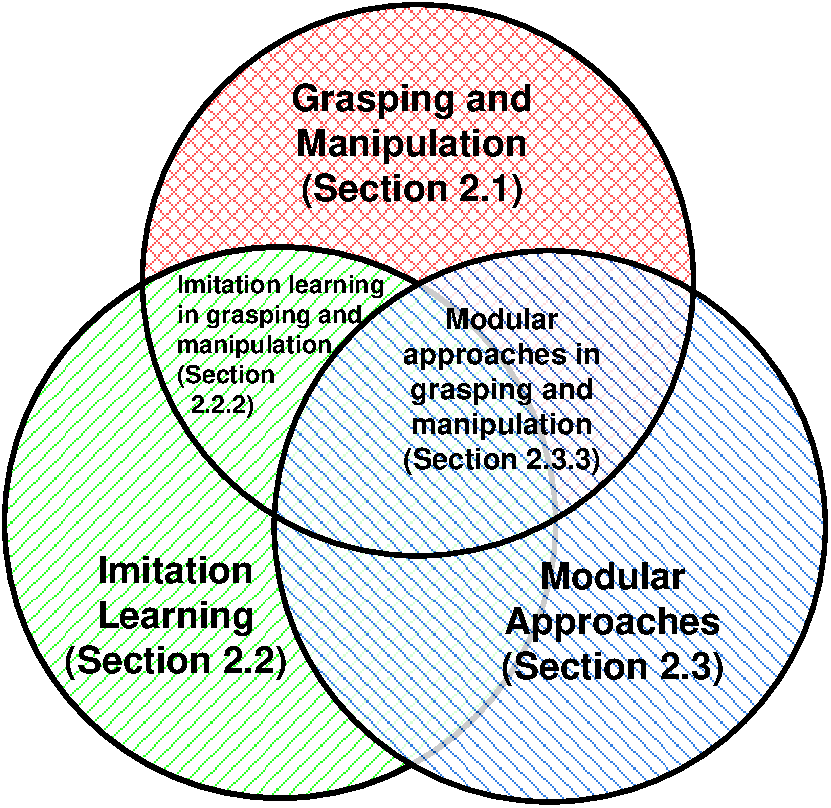
\includegraphics[width=15cm]{./fig_cha2/litreview.pdf}
  \caption{Structure of this literature review. This chapter reviews studies in three areas: robot grasping and manipulation (Section \ref{cha2:sec1}), imitation learning (Section \ref{cha2:sec2}) and modular approaches (Section \ref{cha2:sec3}). Approaches involving imitation learning in grasping and manipulation are reviewed in Section \ref{cha2:sec2:grasping-learning}. Applications of modular approaches in grasping and manipulation are reviewed in Section \ref{cha2:sec3:grasping-modular}.}
  \label{fig:litreview}
\end{figure}


\section{A review of robot grasping and manipulation}
\label{cha2:sec1}
%TODO: introduction  of grasping and manipulation. What is grasping? What is manipulation?
As discussed in the first chapter, grasping and manipulation problems are important but difficult to solve.
Robot grasping and manipulation research aims to enable robots with a human level ability of handling objects. Grasping and manipulation are usually included in the same research category and are studied by the same robotics community, as they both try to tackle the ``contact tasks'', which  use robot hands (end-effectors) to get physical contacts and interact with target objects.
Robot grasping focuses on how to stabilize the target objects with the support from the robot hand. This involves the problem of where and how to place the hand and fingers to contact the targeted objects. Robot manipulation focuses on delivering the targeted objects from the current state to a desired state, which involves the problem of how to apply forces and torques on the object to achieve the desired state. Besides these two problems, one problem is often discussed by the same community -- the reaching problem. How to move the robot hand to reach the object so that the planned grasps or manipulation strategy can be achieved, for example making contacts in the right places to pick up a box, is the problem studied in reaching. In the later three sections, we will present an overview of these three topics.
%TODO: divide to three sections.
%Reaching: forward and inverse kinematics
%Grasping: analysis and synthesis of closure grasps
%Manipulation: prehensile and nonprehensile

\subsection{Robot grasp planning}
\label{cha2:sec1:planning}
%\label{cha2:sec1:grasping:planing}

% ----- What is grasp planning. Force/form closure -----
The studies of robot grasping have two main categories: geometric based planning and control based execution. The first category studies how to pose the hand and fingers form a stable grasp and the latter studies how to execute a grasp plan and how to make local adjustment to correct a non stable grasp. Early studies of grasping mainly focus on the first category and the second category raise increasing interests in recent years. In this review, we will first look into the planning problem and then move to the execution problem.

Given a robot hand and an object, there are an infinite number of ways to grasp the object. These grasps have different performances and functionalities. Grasp planning is usually formulated as an optimization problem of grasp performance, by finding the contact point locations or robot hand configuration. This technique is call optimal grasp synthesis. The most important criteria in the optimization is the stability of the grasp. In the robot grasping literature, two kinds of ``closure'' are the most extensively used mechanisms for guaranteeing stability: the force-closure and form-closure~\citep{Nguyen87}. A grasp is said to achieve force-closure when the fingers can apply appropriate forces on an object to produce wrenches in any direction~\citep{SalisburyJr1985}. Form-closure is a stronger condition than force closure, which can only be achieved if a grasp is force closure with frictionless contact points~\citep{diziouglu1984mechanics}.

% ---- Grasp quality ----
To measure grasp stability qualitatively, the concept of grasp quality is introduced. Various grasp quality metrics are proposed for different purposes. One important concept involves is the ``grasp wrench space`` that the space of the possible force and torque to be applied by the fingers.
%Starting from the idea of minimizing the sum of the contact forces, \citet{li1988task}, \citet{kirkpatrick1992quantitative} and \citet{ferrari1992planning} propose different measurements of the grasp quality based on the hand wrench space.
The concept of ``task ellipsoid'', which is a geometric representation in the wrench space of the force and torque required in a task, is proposed by \citet{li1988task} to measure how suitable is a grasp for the task: the more overlap between the task ellipsoid and the wrench to be provide by the grasp, the more suitable this grasp is.
\citet{kirkpatrick1992quantitative} refer the grasp quality to the ``efficiency'' of a grasp and define it as the ratio of the largest external wrench that can be balanced by at most one unit force at each contact point. Based on the same principle, \citet{ferrari1992planning} define the quality of a grasp to be the minimum distance from the origin of the wrench space to the boundary of the maximum possible grasp wrench.
\citet{trinkle1992stability} propose a test to measure how far is a grasp away from the form closure.
These metrics are ``object-centric'', i.e. they only consider the contact point locations and the object geometry, while the robot hand configuration is not taken into account. \citet{miller1999examples} take one step further: they use a simulation method to compute the grasp quality of a given object and robot hand configuration. They later develop the physical simulator GraspIt! for grasp quality analysis~\citep{miller2004graspit}. Our work in grasp planing described in Chapter~\ref{cha3} is based on this simulator.

% TODO: Some grasp synthesis methods. Add more.
%Optimal force-closure grasp synthesis is a technique for optimizing the grasping performance by finding the contact point locations.
Optimal force-closure grasp synthesis concerns determining the contact point locations so that the grasp achieves the most desirable performance in resisting external wrench loads.
Based on the grasp quality concept, some approaches optimize an objective function according to a pre-defined quality criterion~\citep{Zhu2003,Zhu04} in the grasp configuration space.
%Some techniques compute optimal force-closure grasps by
%optimizing an objective function according to a pre-defined
%quality criterion~\citep{Zhu04, Zhu03} in the grasp configuration space.
These approaches do not take into account the kinematics of the hand. To bridge this gap, \citet{S.ElKhoury2012} propose a one shot grasp synthesis approach that formulates and solves the problem as a constraint-based optimization.

% ----- Learning and modular methods to tame the dimension -----
Multi-finger grasps usually involve a large number of degrees of freedom.
Searching the grasp space for an optimal grasp requires massive computing time considering the huge number of possible hand configurations. To solve this problem, imitation learning and modular approaches are introduced to constrain the searching space. The relevant literatures are reviewed in Section~\ref{cha2:sec2:grasping-learning} and Section~\ref{cha2:sec3:robotics}

% ----- grasping in cluttered environment -----
The above methods are for static grasp planning that rely on precise and accurate object models. These methods are well suited to controlled industrial environments, for example picking up aligned boxes from the assembly line. However, they are not very applicable for service robots working in human dominated environments. For this reason, in recent years the research has shifted to tackle the problem of maintaining grasp stability in dynamic and cluttered scenes. These studies include handling uncertainty and noise in perceptual data and handling unseen (novel) objects and unforseen situations. To tackle the former problem, one approach is to take the uncertainty and noise into account in the planning and generate robust grasps~\citep{brost1988automatic,zheng2005coping,hsiao2011bayesian}.
\citet{brook2011collaborative} try to handle the uncertainties in object shape estimation by finding a common grasp of the few most possible object shapes.
Besides synthesis, grasping motion is also studied~\citep{,kehoe2012toward}, where the uncertainty is handled by the compliant finger motions. For grasping novel objects, different general object shape representations are proposed. The most studied representations are 2D or 3D local features such as edge, contour and color~\citep{saxena2008robotic,detry2009learning,kroemer2010grasping}, combination of shape primitives~\citep{miller2003automatic,huebner2008minimum,el2010new} and exclusive mathematical representation of the global object surface geometry and topology~\citep{el2013generation,pokorny2013grasp}. Local features allow quick computation of grasps on a sub-part of an object, while global representations allow a global search of good grasps with large computation expenses. Planning grasps for novel objects effectively and robustly remains a challenge.



\subsection{Robot manipulation}
\label{cha2:sec1:manipulation}
%\label{cha2:sec1:grasping:manipulation}

% Current state of art in manipulation

%Different from grasping which aim to stabilize a object, manipulation aim to change the object status, usually its position and orientation, from the current one to the desire one.
Manipulation differs from grasping in that it aims to change the object status, usually its position and orientation, from the current one to the desired one, whereas grasping merely aims to stabilize the object.
This means the problem of manipulation is two-fold: controlling the hand movement to control the object movement.
Studies in manipulation can also be split into two topics: manipulation planning and task execution. The former focuses on planning the hand movement, reasoning how to accomplish a complex task by a sequence of motions and behaviours, while the latter focuses on controlling the object movement, answering the question of how to apply force and torque to deliver a target object to the next desired status. The former problem is mostly addressed by learning from humans and extracting motion primitives from human demonstration, which can be used to build complex behavior for accomplishing a task. We will review those works in Section~\ref{cha2:sec2:grasping-learning} that reviews imitation learning and Section~\ref{cha2:sec3:robotics} that reviews modular approaches. In this section we will concentrate on the latter problem of execution.
%Briefly speaking, there are two directions of approaches: the position and force hybrid control method and the impedance control method.
% Impedance: find a good task impedance.
% force/position hybrid: transition

% open challenge -- to verify your contribution
% why need imitation learning? why need modular?

% Difficulty
%The fundamental difficulty of manipulation is that it requires the robot to adapt to the current situation and tackle sudden changes.
%Manipulation is difficult for that it involves the interaction between robot and the environment.

% TODO: hybrid control
Control methods for manipulation can be roughly divided into two groups: hybrid position$\backslash$force control and impedance control. The hybrid control approaches directly control the force and the position of the robot hand \citep{li1989grasping,yoshikawa1993coordinated}. It specify which few directions to control the force and which directions to control the position and control both of them at the same time. On one hand, this simultaneously direct control of position and force allows a precise control of the hand-environment interaction. On the other hand, it requires a fast reaction to task context changes, e.g. transition between contact and no contact, and a small delay in control may cause large force overshot.


% Impedance control
% TODO: virtual spring
In the contrast, the impedance control method indirectly control the force via defining impedance of the hand~\citep{howard2010transferring,wimbock2012comparison}. Given the desired impedance of a task, we can compute proper motor commands for the robot to accomplish it. Fixed impedance control is limited to simple tasks. In many manipulation tasks such as opening a bottle cap, variable impedance is required: at the beginning we need a large impedance to break the contact between the bottle and the cap, and later we need a small impedance to drive the cap smoothly. For such tasks fixed impedance control will either lead to task failure or cause hardware damage.
However, computing the impedance for a given task involving variable impedance is difficult.
In many cases the impedance is roughly approximated by a linear model, but this is inadequate for non-linear tasks.

Variable impedance can be learnt by humans physically correcting the robot impedance, i.e. wiggling the robot arm, in different stages of the task~\citep{kronander2012online}. For learning manipulation, however, wiggling the robot fingers will interrupt the task and may cause task failure.
%This is feasible for learning robot arm impedance but not for object impedance.
Variable impedance can also be learnt by the Policy Improvement with Path Integrals ($PI^2$) reinforcement learning algorithm, with a task specific cost function~\citep{buchli2011learning}. Designing this cost function requires insight into the task and is usually difficult.

% TODO: rolling and sliding -- difficult
Most of these control methods assume fix point contacts between robot and the environment. In reality, manipulation control always involves rolling and sliding between the contact surfaces. The dynamics of rolling and sliding are analysed in various of studies \citep{howe1988sliding,montana1988kinematics}. These needs to be taken into account in order to rigorously implement the control methods. However, an analytical model of friction that can reliably predict sliding can result in stable analysis of the system dynamics is no yet available \citep{bicchi2001robotic}. This makes the manipulation process hard to predict and requires the robot to adapt to the current situation and tackle sudden changes. This inspires us to learn how human adapt to changing contexts and accomplish manipulation tasks. We presents our study in this direction in the Chapter~\ref{cha4}.



\subsection{Reaching motion planning}
\label{cha2:sec1:reaching}
%\label{cha2:sec1:grasping:reaching}

Reaching motion is another key component in the robot grasping and manipulation problem. Given a computed stable grasp, the question to answer in this study is how to deliver the robot hand to the desired position and form the desired hand posture. This is not a simple path planning problem for the robot arm, but a high dimensional planning problem taking the multiple finger movement into account. On one hand, most studies try to plan a motion to avoid premature collisions between the hand and the object. To this end, the finger movement and the arm movement always need to couple in order to ensure the fingers clutch at the right moment \citep{Shukla2011CDS}, and curve around the object to form the desired grasps \citep{kroemer2011grasping}. To increase the robustness of a grasp, the uncertainty in perception is also taken into account \citep{stulp2011learning}. On the other hand, however, some researches study how to deliberately produce ``premature'' contact with the object.

\citet{chang2010planning} study the human ``pre-grasp'' movements such as sliding a coin to the table edge in order to pick it up, and rotating the handle of a pan to a proper position to grasp it. These methods largely increase the chance of successfully executing a grasp by changing the object's status.

\section{A review of imitation learning}
\label{cha2:sec2}
%\label{cha2:sec2:learning}

This section provides a brief introduction to robot imitation learning and then reviews its applications in robot grasping and manipulation.

\subsection{Robot imitation learning}
\label{cha2:sec2:learning}
Since the first study on robot imitation learning~\citep{friedrich1996robot}, this approach has become one of most popular research areas in robotics. It is considered to be a designer-friendly approach to teach robots new tasks. The aim of imitation learning, also referred to as ``Learn by Demonstration'' (LbD) or ``Program by Demonstration'' (PbD) in some literature, is to enable a robot to learn new skills by observing human demonstrations and then to reuse these skills in similar tasks. In recent years, this approach has been extensively studied~\citep{calinon2007learning,calinon2008robot,dillmann2004teaching,kulic2012incremental} as a promising approach to build robot intelligence.

\subsection{Robot learning grasping and manipulation }
\label{cha2:sec2:grasping-learning}
%\label{cha2:sec4:grasping-learning}

%[El-Khoury and Sahbani, 2010].
%\citet{bekiroglu2011assessing} integral the information of the object shape, approach vector, tactile data and joint configuration to estimate a grasp quality.

% Why need to use learning, benefit?
% ----- reduce complexity -----
As discussed in Section~\ref{cha2:sec1},
conventional grasp and manipulation planning methods suffer from the curse of dimensionality.
Learning techniques have been introduced to avoid the complexity of computing kinematical constraints guaranteeing stable grasps. Briefly speaking, robot grasping has two learning sources: imitation learning from human demonstration and learning from data collected from the simulation.
In imitation learning, some researchers use datagloves for human demonstration. The human hand configuration is then mapped to an artificial hand workspace and the joint angles~\citep{Fischer1998,ekvall2007learning}, or hand preshapes~\citep{Kyota2005, pelossof2004svm, Li07} are learnt. Some other researchers use stereoscopy to track the hand when a demonstrator is performing a grasp~\citep{hueser2006learning} or to match the hand shape to a database of grasp images~\citep{Romero2008}. For long term automatic learning, markerless methods to track human hand and arm movements in the approach and grasp execution are studied~\citep{ekvall2007learning,do2009grasp}. These learning based approaches succeed in taking into account the hand kinematics and generate hand preshapes that are compatible with the object features.
Human grasp postures are usually mapped to robot hand postures in fixed schemes, according to the shape of the object and the type of grasp chosen by human.
The learn from simulation method gets around this mapping step: it directly generates grasps with the robot hand's mechanical constraints. For a given object shape and a robot hand, thousands of grasps are generated in the simulator and later used as training data. \citet{pelossof2004svm} use a discriminative Support Vector Machine model to learn the correlation between the grasp configuration and grasp quality, while \citet{bidan2013grasp} use a generative Gaussian Mixture Model to learn the distribution of force closure grasps. Both models are used to generate new grasps. Grasp training data can also be generated in a real robot platform rather than a simulator~\citep{herzog2014learning}. However, this method is much more time consuming and hence it focuses on finding a way to maximize the use of the grasping experience, i.e. generalizing grasping strategies for novel objects.

To further reduce the complexity of the grasping problem, modular approaches are used. This will be discussed in the Section~\ref{cha2:sec3}.

% ----- uncertainty -----
\textcolor{red}{Besides reducing the complexity of the grasping problem, learning approaches are also used to tackle those common problems that appear in the human environment: uncertainty and noise in perception data, novel objects and unforeseeable situations. Most of these learning approaches study how human handle those situations and imitate the strategies.} \citet{ekvall2007learning,stulp2011learning} study human grasp motion and try to learn how humans choose the approach vector that is robust to noise in pose estimation. Driven by the same idea, the human grasp postures are also studied and mapped to robot hands~\citep{tegin2009demonstration}. Inaccurate execution of a grasp can also cause problems. Human handle this issue by using tactile feedback.
With the recent advances in tactile sensing technology, many attempt to include the tactile sensory data in assessing the grasp stability.
After grasp execution, feedback from tactile sensors provide a more accurate estimation of grasp stability then which provided by vision. This allows grasp correction and can avoid failed lifting of the object caused by instable grasp~\citep{li2014learning}.
\citet{bekiroglu2011assessing} integrate the information of the object shape primitive, approach vector, tactile data and hand joint configuration to estimate a grasp quality.
In the later work, contact point locations are also taken into account~\citep{dang2012learning,dang2014stable}. The support vector machine (SVM) is the most used model in discriminating stable and instable grasps. These tactile based methods are also used to evaluate grasps of novel objects.

% ------ novel object ------
%The tactile feedback based methods usually do not rely on predefined object shapes. Hence these methods can be easily applied to estimate grasp quality for novel objects.
Human's ability in generated grasps for novel objects is also studied and imitated.
\citet{detry2009learning} study the human Early-Cognitive-Vision (ECV), which includes colour and edge information that can be used to describe any objects. These features are associated with appropriate grasps and hence grasps of novel objects with matched features can be generated.
\citet{el2007learning} try to imitate the human mechanism of representing objects by segmenting objects into a set of superquadric shape primitives. The mechanism of a human choosing the grasp component is then learnt by a Neural Network~\citep{el2010new}.



% ----- fast adapt -----
The human environment is dynamic and full of perturbations. These perturbations cannot be foreseen and can only be handled when they happen. A learning approach is also used here to provide methods for quick adaptation. Methods are proposed to simplify the generation of grasps such that a moving object can be caught~\citep{harada2008fast,kim2012,bidan2013grasp}
Besides using visual features, tactile sensors can provide additional useful information not accessible by vision. Many methods for quick adaptation to the actual contact conditions are proposed~\citep{hsiao2010contact,hsiao2011robust,kazemi2012robust,sauser2011iterative,li2014learning}.




% --- Manipulation ---
%%% Compare to analytical solution: more robust, but not guarantee
%%The learning approaches generate give precise contact point locations that guarantee grasp stability. Instead, most of them generate a grasp by less specific specifications such as the approaching vector and pre-grasp postures.
%%At the other hand, these learning approaches usually rely on statistical models. Therefor these approaches do not provide guarantee of the performance of the grasp, even if the plan is execute perfectly. The stability of the planned grasps can only be evaluated after execution. However, for the same reason they tolerate a certain amount of noise and are more robust to errors. Hence, these methods are more suited to human dominate environments.
%%
%%Demonstration based learning has been extensively studied~\citep{calinon2007learning,dillmann2004teaching,kulic2012incremental} as a promising approach to build robot intelligence. %It is essential for the tasks that analytical expression of the system is hard to derive.
%%Learning manipulation tasks is one of the main application of this approach. The physical properties of a manipulation task is hard to express analytically, and as a result the control strategy is hard to derive. Modeling expert's demonstration of strategies has been used as an alternative to the analytical solution.
%%
%%Two major forms of demonstration are used in teaching manipulation tasks: kinematics teaching and tele-operation. In kinesthetic teaching, human directly contact with the robot and guide their movements to accomplish a task~\citep{korkinof2013online,pais2014encoding,pastor2011skill,Miao2014}. The trajectory of movements and contact force are recorded by the robot sensors.
%%% ===== Why not kinematics approach? =====
%%This method is simple and effective but limited in the number of controllable end effectors. While a manipulation task usually involves multifinger movement, a human can kinematically operate one finger with each hand and hence two fingers simultaneously at most. To control multi-finger hands, some researchers use tele-operation~\citep{bernardino2013precision,kondo2008recognition,Fischer98}. This usually relies on data gloves and motion capture system to sense human hand-arm motions. The human motion is mapped to robots to generate motions and interact with the environment. In fine manipulation tasks, the robot platforms are usually restricted to anthropomorphic hands for better mapping. All of these methods provide no direct force feedback to the human demonstrator during manipulation.
%%
%%In some studies, the human demonstrate manipulation tasks with their own bodies~\citep{asfour2008imitation}. With direct interaction with the object the human demonstrator is able to perform the task most naturally and with a more delicate control strategy. The task information captured from these human demonstrations needs to be transferred to robots. Various mapping methods have been proposed~\citep{hueser2006learning,asfour2008imitation,do2011towards,}, while human correction~\citep{calinon2007incremental,sauser2011iterative,romano2011human} and self-correction via learning~\citep{bidan2013robio} are proposed as alternative solutions. In general, how to effectively transfer human skills to robots skill remains a challenge.



%machine learning techniques  to the grasping
%problem. Some researchers use datagloves, map human hand to artificial hand workspace and learn the
%different joint angles~\citep{Fischer98,Ekvall07}, or hand
%preshapes~\citep{Kyota05, Pelossof04, Li07}  in order to perform a grasp. Others use
%stereoscopy to track the demonstrator's hand performing a
%grasp~\citep{Hueser06} or try to recognize its hand shape from a
%database of grasp images~\citep{Romero08}.
%However they focus on different problems, such as telemanipulation~\citep{Fischer98} and human hand tracking~\citep{Hueser06}, rather than real time unattended grasping.
%Other group of researches concentrate on generating a list of grasps for one object~\citep{Kyota05, Pelossof04, Li07, saut2011efficient}.


\section{A review of modular approaches}
\label{cha2:sec3}
%\label{cha2:sec3:modular}
This section first briefly reviews the modular approaches studied in cognitive science and control theory, and then concentrates on modular approaches in robotics.

\subsection{Modular approaches in cognitive science}
\label{cha2:sec3:cognitive}
%\label{cha2:sec3:modular:ai}

% TODO: Modular approach in cognitive science (artificial intelligent and neuroscience), control and robotics
%It has also been shown to be an effective architecture of building intelligent systems~\cite{bryson2004modular,BrysonMcG12}.
% MOSAIC
One typical hypothesis of a modular model in motor control is MOSAIC: the Modular Selection and Identification of Control. It is a paradigm of multiple module control, where each module is composed of a forward model and an inverse model. The forward models are responsible for estimating the task context in real time, and the inverse models are used to generate appropriate motor commands for the context. The inverse models are weighted by the accuracy of the estimations of their corresponding forward models. The final motor command is the linear combination of the commands factored by their weights.

\textcolor{red}{TO BE EXTENDED}

\subsection{Modular approaches in control}
\label{cha2:sec3:control}
%\label{cha2:sec3:modular:control}
%Aim: MMAC is good, useful. Discussed for long. Hard to decide -> learning.

% Adaptive control
The use of modular approaches in control theory is different from that used in AI. As discussed above, in the discipline of AI, modularity is needed when building a large complex versatile system. In the discipline of control theory, on the other hand, modular approaches are used to handle the adaptive control problem, which is usually referred to as multiple model adaptive control (MMAC).
\textcolor{red}{I'm not sure that this last sentence explains what the differences really are between a modular approach in AI and a modular approach in control theory}
%It is method to handel .... problems in adaptive control.
Adaptive control is a control method where the controller changes itself to adapt to the changes in the control condition.
A commonly used example is where the controller of an aeroplane adapts to a reduction in the weight of the jet fuel.
Conventional adaptive control methods rely on state estimation. The controller tries to estimate the changes of the system dynamics and then modulates its control parameters to adapt to the changes. For frequently changing environments, however, the period of modulation of the control parameters may cause a transient error, where strong fluctuations can downgrade the performance and damage the hardware. MMAC is used to reduce the transient error by conducting a fast adaption. A MMAC system is usually composed of several different controllers, each particularly designed for one control condition. During the control process, the environment is monitored in real time and one or more controllers suitable for this environment are activated to generate the control command. When the system encounters a sudden change, it will adapt to it by activating another set of controllers. It does not need to re-optimise the control parameters and hence the transient error is reduced.

MMAC dates back to the 1970s. \citet{athans1977stochastic} use multiple Kalman filters in controlling equilibrium flight, to handle sensor errors and to reconstruct the state variables in different flight conditions. The final adaptive control signal is computed by the linear combination of the control signal generated by each model, weighted by the associated probability. Later, a switching MMAC is proposed and its stability is studied~\citep{fu1986adaptive}.
%Switching was first introduced by Martennson1986
%Morse 1993 study stability
\citet{narendra1994improving} use MMAC to improve the performance of the controller in multiple environments, particularly to reduce the transient error that is caused during the transition of the control parameters from one set of optimal values to another. They later use neural networks to build models for the non linear system~\citep{narendra1995adaptation,narendra1997adaptive}. This controller is implemented in a robot manipulator to follow a predefined trajectory and shows improved performance compared to single model control.

To apply MMAC to a practical control problem, the first step is to design how many modules to use and how to decompose the problem space. For linear plants, this problem is addressed by \citet{anderson2000multiple}. They use the concept of Vinnicombe distance 
\textcolor{red}{need reference to Vinnicombe distance}
to decompose the space. Firstly, an initial random starting point is chosen, where a controller is determined. The controller finds its boundary in the neighborhood where its control is acceptably accurate.
\textcolor{red}{do you mean 'unacceptably', or 'still acceptably'? What defines the boundary condition?}
At the boundary, a new starting point is chosen and a new controller is determined. This process continues until the whole space is covered. Based on this method, \citet{lourenco2006learning} 
\textcolor{red}{citation missing}
propose an approach to recognize the new condition and learn new controls online to adapt. These methods, however, only perform well for learn plants.
\textcolor{red}{learn plants? what?}
How to apply MMAC in nonlinear systems remains a challenge.

In robot control, MMAC has many applications for conducting a task in frequently varying environments. These changing environments can be caused by many factors, such as object interactions. Works on this topic include \citet{petkos2006learning} learning multiple inverse models for controlling robots to follow a trajectory with different workloads on the arm; \citet{nakanishi2013spatio} proposing a time-based switching method for robot systems with variable stiffness actuation to handle the different phases of interaction with the environment; the ``eMOSAIC''~\citep{sugimoto2012emosaic} to bring the MOSAIC from simulation to real robot control. In the last work, the performance of MOSAIC under large observation noise is improved by using an optimal control technique. The method is implemented on the 51 DOF humanoid robot CB-i for a squatting task and a carrying load task. As far as we know, this is the first MMAC implementation for a real robot.

Despite the remarkable theoretical accomplishments and many successful applications of MMAC, its application in controlling service robots is not flourishing. Partly this is because robotics always involves non linear control problems, for which the MMAC has not a principle solution.
\textcolor{red}{need to use another phrase here instead of 'not a principle solution'. Do you mean that MMAC is not the ideal solution for non linear control problems?} 
Also, a MMAC controller itself is difficult to design. Control problems in robotics are highly task specific and the service robots are expected to handle a huge number of tasks.
\textcolor{red}{I have changed 'amount' to 'number' in the sentence above. If the thing we are talking about is continuous we use amount (like for milk), but if it is discrete (like biscuits) then we use number as above. End Lesson :)}
 Hand designing a MMAC for these tasks is not cost effective. %Some of the tasks may needed to be end-user defined, that necessitates a simple user-friendly design scheme.

%But how to modularize is still a problem.
%Anderson 2000 how to decide number of modules for linear plan:
%SMMAC decide when to learn a new module online.
%Predictive control with infinite number of modules.

%Robot:
%Narendra 1995 study robot manipulator
%Sethu with multip phases.
%eMOSAIC
%2012_Design of a grasp force adaptive control system with tactile and slip
%
%
%To handle this problem, the multiple model control is introduced in the 1990's ~\citep{narendra1994improving} and later developed~\citep{narendra1995adaptation,narendra1997adaptive}. This approach is inspired by the local expert model introduced by~\citet{jacobs1991adaptive}. This work propose to use local controllers for different subspaces of the system to improve the control performance.
% Talk about basic idea.  1995 in robot manipulator.

% Talk about developement, 1995 in robot manipulator?

% Read review of adaptive control

%Vinnicombe distance to find number of module?

% Vijarkumar's papers?

% multiple control with mixing. different from local expert?


\subsection{Modular approaches in robotics}
\label{cha2:sec3:robotics}
%\label{cha2:sec3:modular:robotics}
In the previous two sections we list a few applications of the modular approach in robotics from the AI and control prospectives. Modular approaches in robotics go further. In recent years, there have been many studies in the modular approach, especially in robot motion planning, grasp planning and manipulation planning. This is mainly due to the trend to try to move robots from the industrial controlled environment to the human dominated environment, where the robots have to handle dynamic and complex situations. In this section, we will give an overview of modular approaches to motion planning. Applications in grasp planning and manipulation will be reviewed in detail in Section~\ref{cha2:sec5:grasping-modular}.
\textcolor{red}{cross reference missing}
Modularities in robotics always refer to ``primitives'', such as ``object shape primitives'', ``motion primitives'' and ``manipulation primitives''. Among these, the most extensively studied area is motion primitives.
To build a versatile service robot that can work in a human dominated environment and assist a human, high level behaviour planning is required. This means robots need to be equipped with the ability to plan a sequence of movements that fulfil a commanded task, such as ``clean the table'' and ``put the food into the fridge''. The conventional method of motion planning is to search in a high dimensional space formed by the numerous degree of freedoms of the robot. The number of possible solutions to accomplish a task is therefore nearly infinite.

This redundancy is useful. In reality various constraints, such as avoiding obstacles, may be added to the task. Due to the redundancy, we are able to find feasible solutions under multiple task constraints. However, this redundancy also makes planning difficult as the search space is extremely large. One common approach is to carry out optimization for the task with constraints that are mathematically equivalent to the task constraints.
\textcolor{red}{you need to check the last sentence as I have changed it to read properly, but the sense may now be wrong}
The drawback of this optimization approach is that defining a proper cost function and proper constraints for the task is not easy. This requires the robot use to process a certain amount of knowledge in mathematics and mechanism, as well as a deep understanding of the task.
\textcolor{red}{rewrite last sentence as I'm not sure what you are trying to say here}
As an alternative, modular approaches can be used to reduce the search space, without discarding good solutions. To this end, the concept of the motion primitive is introduced into robotics. This is a concept from neuroscience research. Neuroscientists have found evidence to suggest that the vertebrate motor system generates motions by combining a small number of motor primitives~\citep{mussa1994linear,mussa1999modular,bizzi2008combining,grillner2011control}. These show the modularized mechanism running in brains: each motor primitive is one module, the combination of many modules generates the complex behaviour.

This idea inspired roboticists to develop simple motion primitives and use them as substrates to develop complex behaviours. In robot motion planning, motion primitives are defined as the most elementary motions, each of which serves one particular purpose. A common way to generate motion primitives is to extract them from human demonstrations: motion sequences demonstrated by humans are discretized to a sequence of motion primitives. Modularized by the motion primitives, the task planning problem is brought from a huge high dimensional search space to a finite discrete space.
They can be reused in other tasks as functional units. %This motion primitive approach has been studied in many literatures~\ref{}.
\textcolor{red}{I don't think you need this sentence. Its obvious.}

% ----- Model motion primitives -----
A great deal of research literature has discussed the use of motion primitives.
\textcolor{red}{Maybe you should cite some here}
Robot motion primitives are learned from humans. These approaches mainly focus on three problems, which are also the typical problems in a modular approach: how to model the motion primitives, how to extract motion primitives from a complex motion sequence and how to combine them to form a complex behaviour.

In studies of the first problem, many roboticists encode the motion primitives with statistical or analytical models, which can be modulated to some extent by varying the parameters according to the requirements of a certain task. The most used modeling methods for motion primitives are The Hidden Markov Model (HMM), mixture models such as the Gaussian Mixture Model (GMM) and the dynamical systems model represented by a set of non linear differential equations. HMM is used to encode temporal motions~\citep{inamura2004embodied,kulic2008incremental,takano2008integrating,lee2010incremental,bidan2013robio}. For time independent motions, \citet{gribovskaya2010learning,khansari2010imitation} use GMM to model multiple human demonstrations in the state space, while \citet{ijspeert2002movement,Ijspeert2003attractor,schaal2005learning,peters2008reinforcement} use nonlinear differential equations to capture an observed behaviour in an attractor landscape. The later is referred as the Dynamical Movement Primitives (DMP), of which the design principle and roadmap is reviewed in \citep{ijspeert2013dynamical}.

% ----- Segmentation -----
Many of the algorithms mentioned above obtain the motion primitives from manual segmentation of motions. However, it is still not clear to us how many motion primitives we need to compose all the human daily behaviours and what these primitives should be. To obtain these primitives, demonstrating all primitives or manually extracting motion primitives from demonstrations is not practical. Even if a library of motion primitives existed, to learn a complex behaviour from human demonstration, a robot still needs to recover the motion primitives from demonstrated motion sequences. Hence, a general automatic mechanism to extract motion primitives is required.

To this end, segmentation of a motion sequence \citep{takano2006humanoid,Pais2013ID879} and clustering of data \citep{kulic2009online,kulic2012incremental} are the most used techniques. These approaches usually rely on a carefully chosen threshold to decide when to segment and stop clustering. A method is to set boundaries on the kinematic variables such as the velocity: \citet{fod2002automated} segment a sequence when a Zero Velocity Crossing (ZVC) is observed. \citet{takano2006humanoid} perform the segmentation according to the correlation among short motions. They first divide the sequence to a set of short notes. When a new motion is demonstrated, they segment it at the moment that the difference between the predicted next note and actual observed one is larger than a threshold. \citet{kulic2008incremental} use a hierarchical clustering method to extract primitives from human motion sequences. Different cut off parameters are tested to evaluate the trade off effect between facilitating quick group formation and introducing misclassification. \citet{Pais2013ID879} extract the primitives according to the variances of the motions in a few demonstrations for a same task. Many other approaches have been proposed to extract motion primitives according to their task requirements. All of these approaches aim to extract a set of motion primitives that are independent functional units and generalized enough to be reused in many tasks. With these pre-defined motion primitives, online recovery of a sequence of motion primitives is feasible. With the presumption of an existence of a motion primitives library we can reduce the segmentation problem to an online motion recognition problem~\citet{meier2011movement}.
%Approaches in this trend mainly have two directions: algorithms with prior knowledge of the motion primitives and and unsupervised algorithms that do not require prior information. The former direction assume an existence of

% ----- Combine -----
The intention of modelling motion primitives is to use them to help with the motion planning problem. According to the task, the use of the motion primitives can be in the form of selecting, mixing or sequencing. The selecting and mixing are for adaptive behaviour: the robot needs to select one or mix a few motion primitives according to the current task context such that it can finish the task.
%Hence another important trend of study is using primitives to form useful behaviors.
%The ``combination'' has two main forms: selecting and mixing.
Selection can be decided by a pre-learned correlation between the primitives and the task contexts: the highest correlated primitive with the current task context is the one to choose~\citep{takano2006primitive}. On the top of this, \citet{daniel2013learning} use Relative Entropy Policy Search (REPS) to optimize the joint state-action distribution and hence choose the optimal set of parameters for the primitive.
Some others choose the primitive that can result in a system state closest to the desired next system state~\citep{hauser2008using}. A similar idea is used in the mixing method, where more than one motion primitive can be activated at the same time. The weight of each motion primitive is computed to make sure the resulting motion can bring the system to the desired state~\citep{bidan2013robio,sugimoto2012emosaic}. From the human robot interaction perspective, the robot should be able to understand human verbal commands and plan the action. \citet{takano2008integrating} propose a method to associate morpheme words with motion primitives. This potentially enables the robots to understand human commands and plan motion by parsing the sentence.




\subsection{Grasping and manipulation by modular approaches}
\label{cha2:sec3:grasping-modular}
%\label{cha2:sec5:grasping-modular}

Modular approaches in robot grasping and manipulation to reduce the problem complexity. Modularization in grasping and manipulation are mainly done in two approaches: modularize by perception and modularize by action. Perceptual modules are mainly used in planning, while action modules are mainly used in execution.

\paragraph{Modularize by perception}
~\\
The first step of making a plan of grasping and manipulation is observing the object. Most of grasp stability analysis are done based on the shape of an object. In human dominated environment, the possible shapes of objects to grasp and manipulate is infinite. Conventional methods to model these object are only effective in convex models. For highly non-convex shapes, local vision features such as edges and colors are used to generate grasping plans at the local areas. To generate grasp for the whole object, \citet{miller2003automatic} propose a modular approach, i.e. planning grasps by shape primitives. The key idea is to approximate a complex object, e.g. non-convex shape, to a set of shape primitives such as boxes, cylinders and spheres. Planning on these shape primitives is relatively easier or pre-trained. Therefore the complex planning problem is tamed to a set of simple problems. According to different purposes, different shape primitives are proposed. \citet{miller2003automatic} use four primitives including box, cone, cylinder and sphere; \citet{huebner2008minimum} use minimum bounding box to decompose an object and \citet{el2010new} use superquadric as the shape primitive. These methods are based on the complete object point clouds, which may not be fully accessible in the real scenario. Methods to split objects to shape primitives and detect primitives parts are proposed, which mainly exploit the techniques in graphics such as the RANdom SAmple Consensus (RANSAC)~\citep{garcia2009fitting,gallardo2011detection}.
\citet{faria2012extracting} use multiple sensors to track human hand trajectory and tactile data, and hence extract motion primitives and contact primitives from the demonstration. These information is then merged to form a object probabilistic volumetric model, which is decomposed to multiple superquadrics.

\paragraph{Modularize by action}
~\\
The motion primitive concept is also introduced to grasping and manipulation. These differ from the reaching movement primitives discussed in the previous Section~\ref{cha2:sec3:modular:robotics}, where the goal is to reach the targeted points. The grasping and manipulation motion primitives are more task-oriented, i.e. each primitive is associated with a specific impact on the environment, such as getting contact with the object and pushing the object. Therefore in the literature these primitives are sometimes referred to as ``task primitives''. Because of the variety of tasks and their complexity, these task primitives are usually manually defined. Transitions between them are usually decided by contact events that indicate the impacts on the environment~\citep{morrow1997manipulation}. \citet{michelman1994forming} propose the representation of the relationship between task primitives by a finite state machine. \citet{kazemi2012robust} define three task primitives for force compliant grasping of small objects from a table top. The Dynamical Movement Primitives (DMP) mentioned previously, which model desired motion by an attractor landscape, is extended to deal with various problems when executing a grasp. The combination of the DMP and the Early Cognitive Vision Descriptor (ECVD) for grasp planning enable a robot to plan the path of  approach of the hand and the finger to avoid premature contact between finger and object~\citep{kroemer2011grasping}. Taking the object poses distribution into account, a new optimization method of the DMP is proposed to find an approach trajectory that produces robust grasps with object pose uncertainty~\citep{stulp2011learning}. Later simplify version of DMP is used to learn movement goal and hence can quickly change the end point location to adapt to the object shape~\citep{stulp2011learning,stulp2012reinforcement}.
\textcolor{red}{cannot fix last sentence as don't know what you mean - sorry}

A number of frameworks are proposed to model and organize the task primitives. \citet{laaksonen2010embodiment,felip2013manipulation} propose a hierarchical framework to solve the embodiment problem of sharing experience among different robot platforms. This is done by defining task primitives in an abstract layer and an embodiment layer.
\textcolor{red}{defined in two layers then? Should it say ...in both an abstract layer and an embodiment layer}
The former can be translated to the latter. This enables the robot to plan tasks with the higher level abstract primitives, and execute them with the embodiment specific task primitives. To facilitate manipulation motion planning, \citet{barry2013manipulation} use a Rapidly exploring Random Tree (RRT) to sequence motion primitives. \citet{detry2013generalizing} modularize a grasp planning task by two constraints: gripper constraints and task constraints. While the former modules handle grasp stability, the latter modules select grasps from the task requirements.

Besides task-specific motion primitives, modular approaches are also used to tame the complex grasp planning problem. The concept of ``hand synergies'' for example, is a modular approach originating in neurophysiological studies~\citep{santello1998postural,santello2000force}. In this field of study, roboticists try to understand how the human central neural system (CNS) simplifies the grasping strategy and how to mimic this mechanism in robot systems. This concept is used in grip force control \citep{gabiccini2011role} as well as grasp planning \citep{gioioso2013mapping}. Similar to this idea, robot ``Eigen grasps'' have been proposed to study the modularity in robot embodiment. Instead of directly searching for good grasps in the high dimensional configuration space of robotic hands, this space can be reduced by generating a set of grasp starting positions, hand preshapes~\cite{miller2003automatic} or eigengrasps~\cite{Ciocarlie2009} that can then be tested on the object model. Such approaches reduce the dimensionality of the hand configuration space, but doing so implies a corresponding reduction in the accessible hand postures.



%This involve not only the studies of the redundancy in human hand mobility but also the redundancy in human cutaneous and kinaesthetic perception. With the recent rapid development of tactile sensors, robots are equipped with more delicate tactile perception. How collect sensation information from these tactile receptors is also a hot topic in robot synergies. In once word, the study of robot sensorimotor synergies aim to find out the modularity in human muscles, joints, fingers, receptors so as to enable robot working in complex and dynamic system.
% Eigen grasp

%TODO: Problem need to solve in modular approach


%In robot grasping, modularity is also studied. In general, planning a grasp for a multifinger robot hand and a given object shape is a computational expansive task, especially for anthropomorphic robot hand with numerous number of joints. XXXXX~\ref{} proposed the concept of ``eigengrasp'' to simplify the grasp planning problem: three different preshapes of the hand are tested to grasp different objects. Approaching the object with a particular preshape until touching, the hand clutch around the object to form a grasp. XXXXX of objects are successfully grasped by one of the three preshapes. This modular approach reduce the complex grasp planning problem to a simple 3-class classification: one only need to classify with preshapes needs to be used for the target object and decide the approach direction.



%\input{includes/cha2_sec4_grasping-learning}
%\input{includes/cha2_sec5_grasping-modular}
%\section{Imitation learning and modular approaches}
\label{cha2:sec6}

\subsection{Motion primitive}
%\label{cha1:modular:motionprimitive}


%TODO: Hierarchical clustering for motion primitives 






\chapter{Modular approach in grasp planning}
\label{cha3}

\section{Introduction}
\label{cha3:sec1}
%%%%%%%%% TODO: extend this to unfamilar object %%%%%%%%%


Given an object and a multi-fingered robotic hand,
generating a set of contacts on the object's surface which ensure grasp stability while being feasible for the hand kinematics is a common problem in grasp synthesis. Over the last few decades, robot grasping has been a popular topic and numerous approaches for grasp planning have been proposed~\cite{sahbani2011overview}. Most of these approaches adopt iterative methods, which are usually able to find a solution within a finite number of iterations and the average computation time is usually in the scale of a few to tens of seconds. However the number of iterations required grows quadratically with the size of the problem and this creates an uncertainty of the time for the robot to plan a grasp. The upper bound of the computation time is barely analyzed in the literature.

%However, most of these approaches adopt iterative methods, which are usually computationally expensive due to the high-dimensionality of the configuration space and the non-linearity of the problem constraints. They are generally able to find a solution, sometimes within a finite number of iterations. Further, they generally try to solve the grasping problem in a static environment. Few of them consider a dynamic environment.

Moving from the traditional engineering environment into a human dominated environment necessitates a fast grasp planning strategy to respond in real time. For example, when reaching out to grasp an object, a robust grasping strategy must be able to adapt rapidly to external perturbations that can modify the initial object position and orientation relative to the robot hand. In the case of catching a flying object~\cite{kim2012}, the robot has only a few milliseconds to plan a grasp before the object touches the floor.

Another application is receiving objects handed over by humans with a robot hand~(Fig.~\ref{handover}). In many circumstance the object must be grabbed quickly: one such example is when the object is heavy or hot; other examples involve time-pressing situations, e.g. in surgery a robot assistant must react sufficiently quickly to doctors handing back implements to ensure smooth running of the surgery.

Besides human-robot interaction, real time planning for the pick-and-place task in the industrial environment may also be necessary: spare parts could be randomly placed on the conveyer belt.
The conveyer belt runs constantly at a high pace and leaves no time for the robot to stop its action and replan.
The robot must therefore respond swiftly to avoid incurring delays in production. Given the limited computational power available on computers embedded in the robot, a computationally expensive algorithm would result in a prohibitively long decision time, leading to task failure in the above scenarios.

Because of the complexity of the problem, real time grasp planning has not been extensively studied. To tackle this problem, we propose a closed-form solution which requires at most three steps to compute a new grasp, and hence guarantee a short computation time and the uncertainty is reduced to the largest extent. In this chapter, we first present a real time grasp planning strategy for familiar objects (Section~\ref{cha3:sec2},~\ref{cha3:sec3}). We then present an extension of this method to plan grasps for novel objects.


%constantly running conveyer belt to deliver to the robot, which does not stop to let the robot plan the grasps. With the limited computational power of an embedded robot computer, a computationally expensive algorithm would result in a prohibitively long decision time, leading to task failure in the above scenarios.

%In many real world scenarios, a rapid grasp planning strategy is required. For example, when reaching out to grasp an object, a robust grasping strategy should be able to adapt rapidly to external perturbations that can modify the initial object position and orientation. In catching a flying object~\cite{kim12}, the robot has to plan a grasp within a few milliseconds before the object touches the floor. Another major application is human handing over objects to robots ~(Figure~\ref{handover}). Human would normally expect their partners to grab the object quickly, especially when the object is heavy or hot. In fact, in many occasions tasks are time-pressing, e.g. in a surgery the doctors hand over tools to the robot assistant and the robot has to react sufficiently quickly to keep the surgery running smoothly. Besides human-robot interaction, real time planning for the pick-and-place task in the industrial environment is also necessary: spare parts could be randomly placed on the conveyer belt to deliver to the robot, which does not stop to let the robot plan the grasps. With limited computational power of an embedded robot computer, a computationally expensive algorithm will have a long decision time and could lead to task failure in the above scenarios.

\begin{figure}
  \centering
  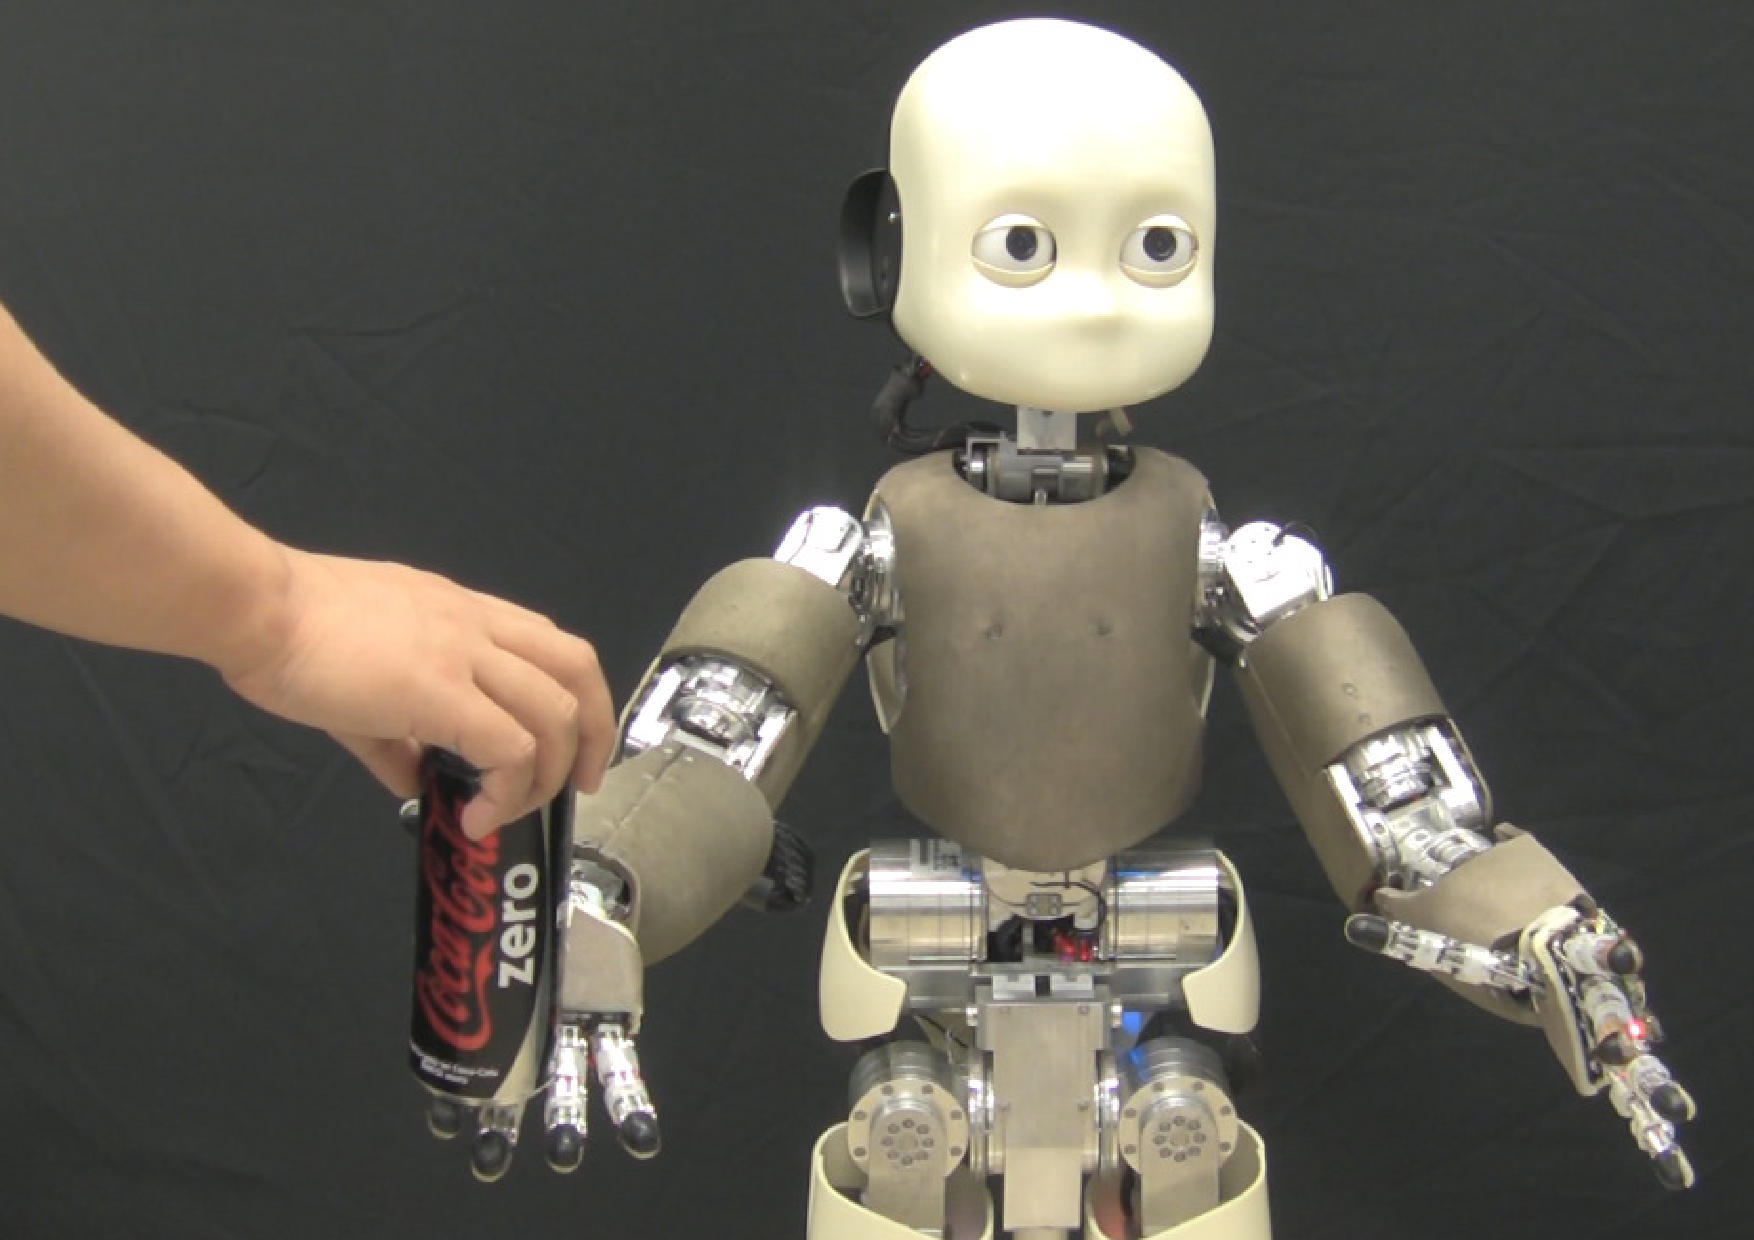
\includegraphics[width=12cm]{./fig_cha3/handover.pdf}
  \caption{A human hands a can to an iCub}
  \label{handover}
\end{figure}



\section{Fast grasp planning for familiar objects}
\label{cha3:sec2}

Traditional manipulation planning strategies usually involve inverse kinematics and optimization, which are computationally expensive. The reported computation time varies from 0.1$sec$ to a few minutes. Recently, there have been some attempts to tackle the problem with real time solutions. \citet{Richtsfeld2008} use a laser scanner to detect cylindrical shapes and plan grasps. This method is limited to cylindrical objects. Kanehiro et al.~\citep{harada2008fast} use approximation models of the friction cone and roughly estimate the force closure criterion. However, this approximation may limit their solutions. In the planning step, they use random sampling techniques to generate grasping postures and loop through the samples to find a grasp satisfying all the kinematic constraints. The reported computation time varies from 10$sec$ to 25$sec$ including path planning of the arm using a 2GHz core.
Daoud et al.~\citep{daoud2011fast} employ a genetic algorithm optimization approach to provide an initial grasp before online manipulation. This evolutionary approach relies on several iterations of optimization before reaching the solution. The reported time is 12.61$sec$ for a spherical object with a 2.2GHz core. The latter two methods, due to their iterative approaches, do not guarantee fast computation in all cases. In contrast, with our closed-form solution the computation time is bounded within a few milliseconds.

We avoid using these by adopting a learning approach.
Our method for planning grasps for familiar objects starts by generating a training dataset of stable grasps for the objects. A $Gaussian$ $Mixture$ $Model$ (GMM)~\citep{cohn1996active} is learned from the data, and the target pose is predicted via $Gaussian$ $Mixture$ $Regression$ (GMR). Hence there is no inverse kinematics computation nor iterative optimization in our method. Generally speaking, our approach is to:
\begin{enumerate}
\item Generate a set of stable grasping demonstrations for a given object and a robot hand (Section~\ref{cha3:sec2:demonstration}).
\item Build a statistical model for the training dataset offline (Section~\ref{cha3:sec2:learn}).
\item Use the model to quickly generate a new grasp, given a starting object-hand configuration (Section~\ref{cha3:sec2:plangrasp}).
\end{enumerate}

\subsection{Grasp generation given the hand kinematics}
\label{cha3:sec2:demonstration}

Two robot platforms available in our lab are chosen to perform the grasping tasks: the iCub and the Barrett hand. The iCub has an anthropomorphic hand with 9 degrees of freedom: 3 in the thumb, 2 in the index, 2 in the middle finger, 1 in the ring and little fingers and 1 for the adduction/abduction movement (Figure~\ref{fig:robothand}(a)). The Barrett hand is an industrial grasper with 3 fingers and 4 degrees of freedom: 1 for each finger and 1 for the separation between the second and the third finger (Figure.,~\ref{fig:robothand}(b)). These two platforms differ drastically in the range of motion for each finger and provide very different grasp demonstrations. They will hence grasp objects in very different ways.

\begin{figure}
  \centering
  \subfloat[\scriptsize{iCub hand}]
  {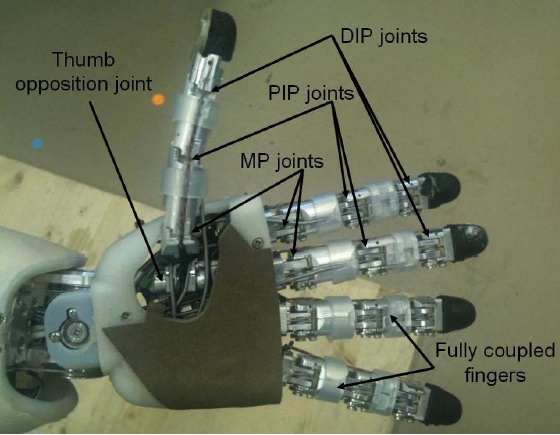
\includegraphics[height=4.5cm]{./fig_cha3/icubhand.jpg}}
  \subfloat[\scriptsize{Barrett hand}]
  {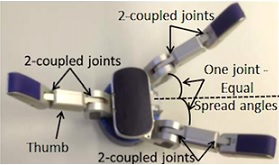
\includegraphics[height=4.5cm]{./fig_cha3/barretthand.jpg}}
  \caption{Two robot platforms used in this work. This method is not bounded to these two robots. It can be applied to any other robot hands given their kinematics.}
  \label{fig:robothand}
\end{figure}

Starting from the geometry of an object and the kinematic property of a robot hand to compute a feasible grasp is time consuming. To achieve fast planning, we do this computation offline. There are numerous possible ways to grasp one object depending on the task's needs~\citep{sahar2012,el2013generation}. To encapsulate all the possible ways, a large amount of training data is needed. Collecting this amount of data on a real robot is time consuming. Therefore, instead of using a real robot, we generate training data by synthesis.

Two different approaches are used here: optimization and simulation. We use a simulation method for the Barrett hand and an optimization method for the iCub hand. In simulation, we use a trial-and-error approach: in the state space we try to generate as many grasps as possible and select those feasible ones. In principle we can generate more variety of grasps by this method, as some of them might be hard to reach by optimization. The 4 d.o.f Barrett hand is particularly suitable for this approach. For the 14 d.o.f iCub hand, however, the state space is much larger and hence the trial-and-error approach is expensive. Instead, for the iCub hand we use an optimization method.


%\subsubsection{Optimization}
\paragraph{Optimization}
~\\
We use the optimization algorithm proposed in the work of El-Khoury and etc.~\citep{el2013generation} to generate grasps for the iCub.
The iCub hand is modelled in 8 dimensions in this algorithm and the thumb, index and middle finger are taken into account.

This optimization algorithm formulates the problem as a constraint-based minimization for a set of hand configuration parameters (hand position \textbf{\emph{h}}, hand orientation {\textbf{\emph{o}}} and finger joints {\boldsymbol{$\theta$}}). These parameters are subjected to a number of constraints to satisfy the following criteria:

\begin{enumerate}
\item The grasp is kinematically feasible for the robot hand;
\item The grasp is a force-closure grasp;
\item The robot hand is not penetrating the object;
\item The robot fingertips contact the object surface;
\item The force provided by the robot hand is able to raise the object.
\end{enumerate}


The iCub's finger joints can only apply a limited amount of torque.
The less joint torque required, the easier it is for the iCub to lift the object. For this reason, we choose the objective function to be the minimum joint torque required to balance the gravity wrench, formulated as:
\begin{equation}
J(\boldsymbol{h},\boldsymbol{o},\boldsymbol{\theta})=\Arrowvert \sum_{i,j} {{\tau}^j_i}\Arrowvert
 \label{quality}
 \end{equation}
where {$\tau$}$^j_i$ is the $i$th joint torque of the $j$th fingers under the force feasibility constraints:

\begin{equation}
 {\tau}^j_i \in [\bar{\tau}^j_i, \hat{\tau}^j_i]
 \label{quality}
\end{equation}
where $\bar{\tau}^j_i$ and $\hat{\tau}^j_i$ are the lower and upper boundaries of $\tau^j_i$.
Minimizing this cost function is equivalent to minimizing the energy required in the joint space in order to accomplish the grasping task.
%As different grasps can cost similar amounts of energy, this objective function has many local optima and hence can provide a large set of different grasps.

The optimization is solved by the Interior Point OPTimizer (IPOPT) method proposed by W\"{a}chter and Biegler~\citep{wachter2006implementation}, written in the AMPL Model Language for Mathematical Programming. To generate a variety of grasps, we exploit the fact that the IPOPT solver converges to local solutions. We provide the solver with a large number of initial conditions, varying from 1000 to 2000. From these initial conditions, which are located in different areas of the space, the IPOPT converges to their corresponding local optima. By this means 500 to 1000 optimized grasps for an object can be obtained. They will be used as the training data in the next phase. The average computation time for the IPOPT to converge to one solution is 2.65$sec$, with a standard deviation of 1.82$sec$. As additional information, the quality $Q$ of each optimized grasp is calculated in the form described in~\citep{ponce1997computing}:

\begin{equation}
Q =\Arrowvert \frac{1}{3}\sum_{j} {\boldsymbol{c}^j}\Arrowvert
\vspace{-0.1in}
\end{equation}
where \textbf{\emph{c}}$^j$ is the contact point (i.e. fingertip) position of the $j$th finger. Though it is not included in the optimization, the quality is used in the comparison between the training set and the result set shown in Section~\ref{cha3:sec3}.
%\textcolor{red}{I don't understand how you can sum the contact points (positions as vectors?), to achieve a quality metric. Maybe the commented out text below provides the explanation required here?}
%, by the distance from the grasp polyhedron to the center of mass of the object:

%To measure the quality of the optimized grasps, the quality $Q$ is calculated as described in~\citep{ponce1997computing}, by the distance from the grasp polyhedron to the center of mass of the object:

To ensure the robot fingertips contact the object surface, the object has to be expressed by an implicit equation. For example, a cylinder can be expressed as:

\begin{equation}
{\left(x^2+y^2\right)}^{10}+z^{20} = 1
 \label{equ:cylinder}
\end{equation}

This expression is in the form of superquadrics, which will be explained in detail in the Section~\ref{cha3:sec4:pgdistribution}.

During optimization, this will be used as a hard constraint for the all the fingertip positions.
For more complex shapes, the implicit equation can be learned by a Gaussian process~\citep{el2013generation}.

The algorithm above can generate a variety of high quality force-closure grasps for a given robot hand kinematic structure and an object model. Since IPOPT is a continuous optimization solver, generating grasps on complex objects requires a continuous implicit representation of the whole object surface model.

%Representing complex objects as an assembly of superquadrics induces a discontinuity in this model preventing IPOPT from converging to a feasible solution.
%An implicit object representation for grasp generation using optimization will be addressed in our future work. This paper will only focus on grasps generated, for the iCub hand, on simple shaped objects such as a cylinder and cuboid.



%\subsubsection{Simulation}
\paragraph{Simulation}
~\\
%TODO: quality criterion: Ferrari and Canny
As the Barrett hand is modelled in the widely used simulator GraspIt!~\citep{miller2004graspit}, we use simulation to generate its data. GraspIt! is designed for grasp analysis and it provides a library of robots and object models. Its quality measurement module computes the grasp quality according to all the contacts between the hand and the object, in the form described by Ferrari and Canny~\citep{ferrari1992planning}. A grasp planning module for primitive shapes, i.e cylinder, sphere, cuboid and cone, is available, allowing users to easily generate grasps~\citep{miller2003automatic}.
To sample grasps for objects with complex shapes, we alter the module and generate grasps as follows.

\begin{figure}
  \centering
  \subfloat[\scriptsize{Initial distribution}]  {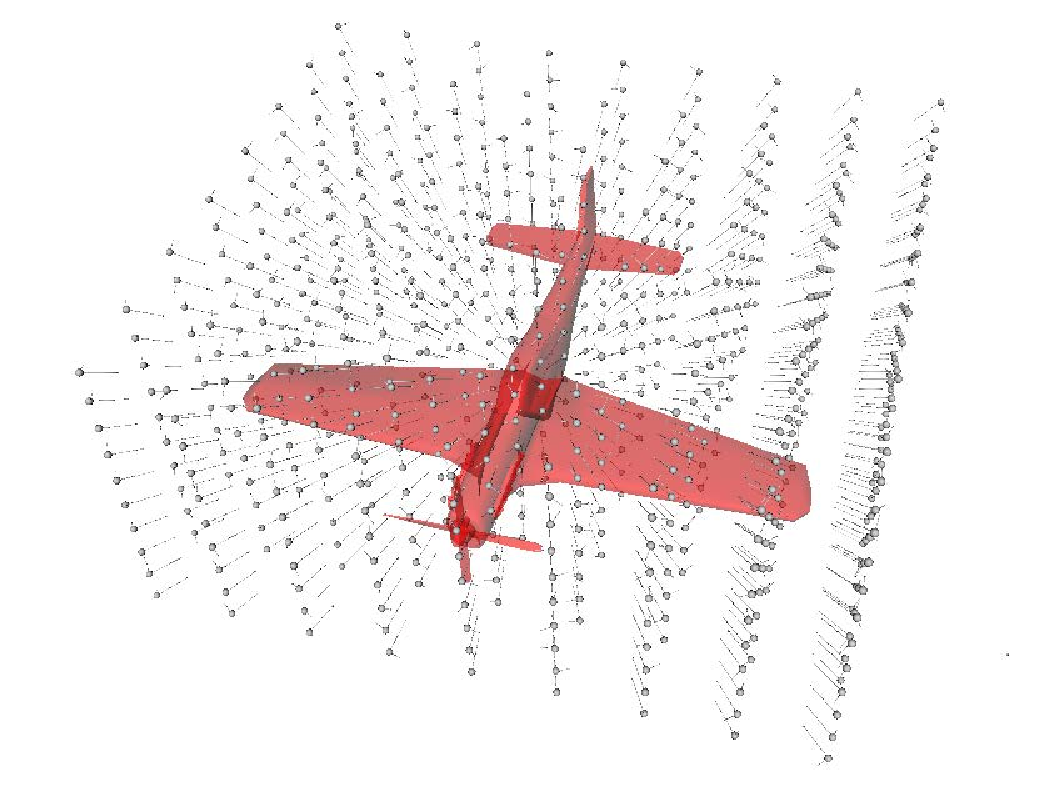
\includegraphics[width=7cm]{./fig_cha3/plane_x2_lattice1.pdf}}
  \subfloat[\scriptsize{Final distribution}]  {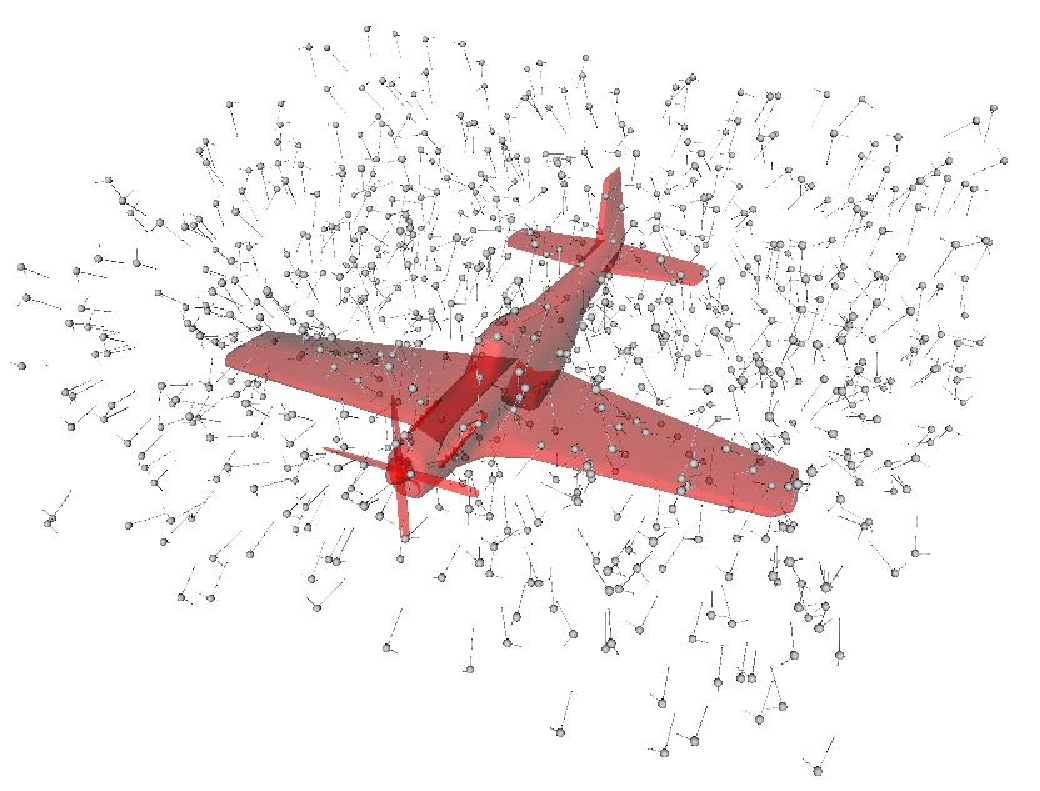
\includegraphics[width=7cm]{./fig_cha3/plane_x2_lattice2.pdf}}
  \caption{\scriptsize{An illustration of part of the grasp position lattice of an aeroplane model. Each grey dot in the lattice represents one robot hand position. The long arrows at each dot represent the hand normal directions and the short arrows represent the fix finger directions. The hand normals are initialized by pointing toward the center of the object, as shown in (a). A small random variance is then added to each grasp later to even the distribution and the final distribution is shown in (b).}
}
    \label{lattice}
\end{figure}

Firstly a robot hand position ``lattice" is generated. Each vertex in the lattice represents one robot hand position, where the hand will be placed to grasp the object (Figure~\ref{lattice}). The object is located in the center of the lattice surrounded by the grasping positions. All palm normals are initially pointing to the center of the object. Random finger separation angles are assigned to each point to form a list of grasp configurations for testing. According to the object size, 1000 to 20000\footnote{More complex and bigger shapes need more testing points.} testing grasps can be generated to ensure that the entire object is surrounded by the lattice and the farthest point to grasp the object is included. The density of the hand position lattice depends on the object shape. Objects with sharp edges, where the normals on the surface change sharply, should have a higher lattice density compared to those with smooth surfaces.

In the final step before testing, small random perturbations are added to each grasp so that the testing points are evenly and continuously distributed in all dimensions.
To test these grasps, the hand is first placed at each position on the test list with the desired posture (hand orientations and finger joints). Next, the fingers clutch around the object until contacts or joint limits prevent further motion. We then use the quality measurement module to compute the quality of each grasp. The non-zero quality grasps, i.e. force-closure grasps, are recorded and used as training data. Note that not all the testing grasps result in feasible grasps. Points causing collisions are removed from the list and only the force-closure grasps are kept as the training data. The average generating rate for the feasible grasps is roughly one per five seconds.

The Barrett hand has one joint in each finger. These three joints can only rotate in one direction and how much they rotate is determined by the object surface, given the hand position, orientation and the separation angle.
Therefore we drop this redundant information and model a Barrett hand grasp only with the hand position, hand orientation and the finger separation angle. The robot kinematics is programmed into the simulator and all simulated robot movement is feasible.

The above two methods can be used to generate both simple shapes and complex shapes. The size of the generated training data varies from 500 to 1600 (Table~\ref{result}). Each training dataset is split into 5 groups for the 5-fold cross validation in the later step.


\subsection{Model learning}
\label{cha3:sec2:learn}

The second phase of the approach is to build a model $\varOmega$ for the grasp demonstrations.
A $Gaussian$ $Mixture$ $Model$ (GMM) is used here to get a probabilistic encoding of the joint distribution $p$(\textbf{\emph{h}},\textbf{\emph{o}},\textbf{\emph{$\theta$}} \text{\textbar} $\varOmega$).
We choose to use GMM because of its ability to effectively extrapolate the missing data, as has been exploited in many applications~\citep{calinon2007learning,sauser2011iterative}. It also has the advantage of capturing the non-linearity of the space, as well as determining how likely a point in the input space is under the model.
The ability to estimate the likelihood of an input query point is crucial: an inference far away from the region covered by the training data can be unreliable, resulting potentially in an infeasible grasp. With GMM we are able to make sure that each input query point is located in or projected to a reliable region (this is explained in the next phase).

Therefore, in the grasp planning phase, we first make sure that a new query point locates in a reliable region by checking its likelihood.
Given a set of sample grasps represented by the hand position \textbf{\emph{h}},  orientation \textbf{\emph{o}} and the finger configuration \boldsymbol{$\theta$}, we model the distribution with a GMM as a sum of $K$ Gaussian components:

%$\xi$\{{\bf {\em h}},{\bf {\em o}},{\boldmath$\theta$}\}, we build our statistical model as a GMM:

\begin{equation}
{
P (\boldsymbol{h},\boldsymbol{o},\boldsymbol\theta \text{\textbar} \varOmega)
= \sum_{k=1}^K {p_{k}p(\boldsymbol{h},\boldsymbol{o},\boldsymbol{\theta} \text{\textbar} {\boldsymbol{\mu}_k}, {\boldsymbol{\Sigma}_k})}
}
\end{equation}
where $k$ is the number of Gaussian components, $p_k$ the prior of the Gaussian component and the $\boldsymbol{\mu}_k$, $\boldsymbol{\Sigma}_k$ the corresponding mean and covariance as:

\begin{equation}
{
\boldsymbol{\mu}_k = \begin{pmatrix}    \boldsymbol{\mu}_{h,k}     \\
                                        \boldsymbol{\mu}_{o,k}          \\
                                        \boldsymbol{\mu}_{\theta,k}
                    \end{pmatrix}
\hspace{0.2in}
\boldsymbol{\Sigma}_k = \begin{pmatrix}     \boldsymbol{\Sigma}_{hh,k}  & \boldsymbol{\Sigma}_{ho,k} & \boldsymbol{\Sigma}_{h\theta,k}  \\
                                            \boldsymbol{\Sigma}_{oh,k}  & \boldsymbol{\Sigma}_{oo,k}  & \boldsymbol{\Sigma}_{o\theta,k} \\
                                            \boldsymbol{\Sigma}_{\theta{h},k}   & \boldsymbol{\Sigma}_{\theta{o},k}   & \boldsymbol{\Sigma}_{\theta{\theta},k}
                        \end{pmatrix}
}
\end{equation}

A GMM approach requires that the data space is locally convex. For a complex object shape, however, the grasp space of hand configuration --- coupled with the finger joint space and constrained by the geometry of the object surface --- may be a non-smooth manifold. In both of the data generation methods described above, we evenly distribute the testing points so as to reduce the possibility of missing small good grasp regions. By these means we obtain most of the possible grasps for the object and approximate a locally convex data distribution, which is suitable for a GMM.

Before training we 1) convert all data into the object reference frame and 2) normalize the data so that all dimensions have a zero mean and a unit variance. Initialized by the K-means, the $Expectation$-$Maximization$ $algorithm$ (EM)~\citep{dempster1977maximum} is used to find the value of $\boldsymbol\mu$ and $\boldsymbol\Sigma$ that maximizes the probability of the training data under the GMM. The number of Gaussian $K$ is selected by the $Bayesian$ $Information$ $Criterion$ (BIC) and verified by 5-fold cross validation to make sure the model is not overfitting (Figure~\ref{bicxv}).

\begin{figure}
  \centering
    \subfloat[\scriptsize{BIC}]  {\label{fig:reachableSamplesPos}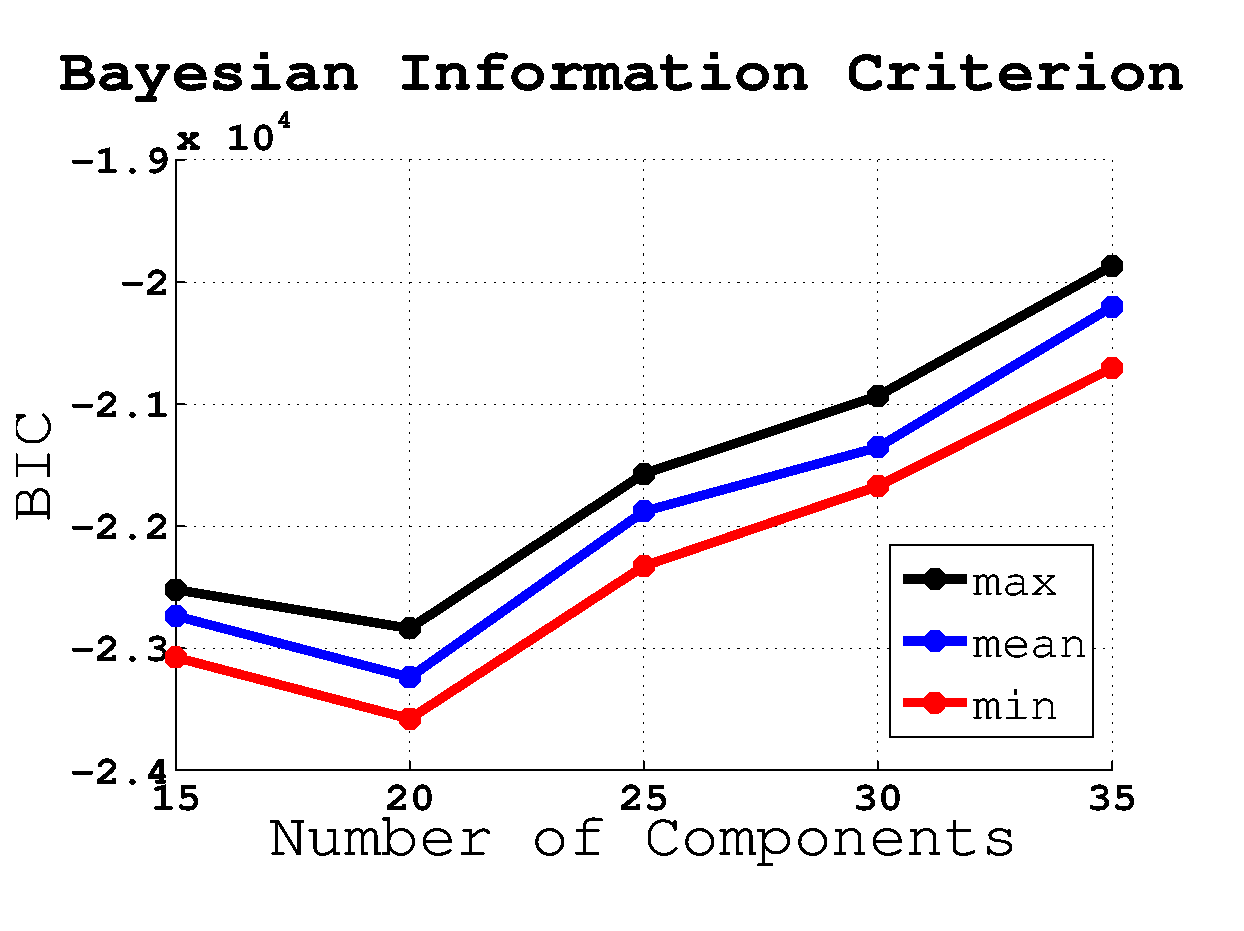
\includegraphics[width=7cm]{./fig_cha3/BIC.eps}}
    \subfloat[\scriptsize{5-fold cross validation}] {\label{fig:reachableModelPos}  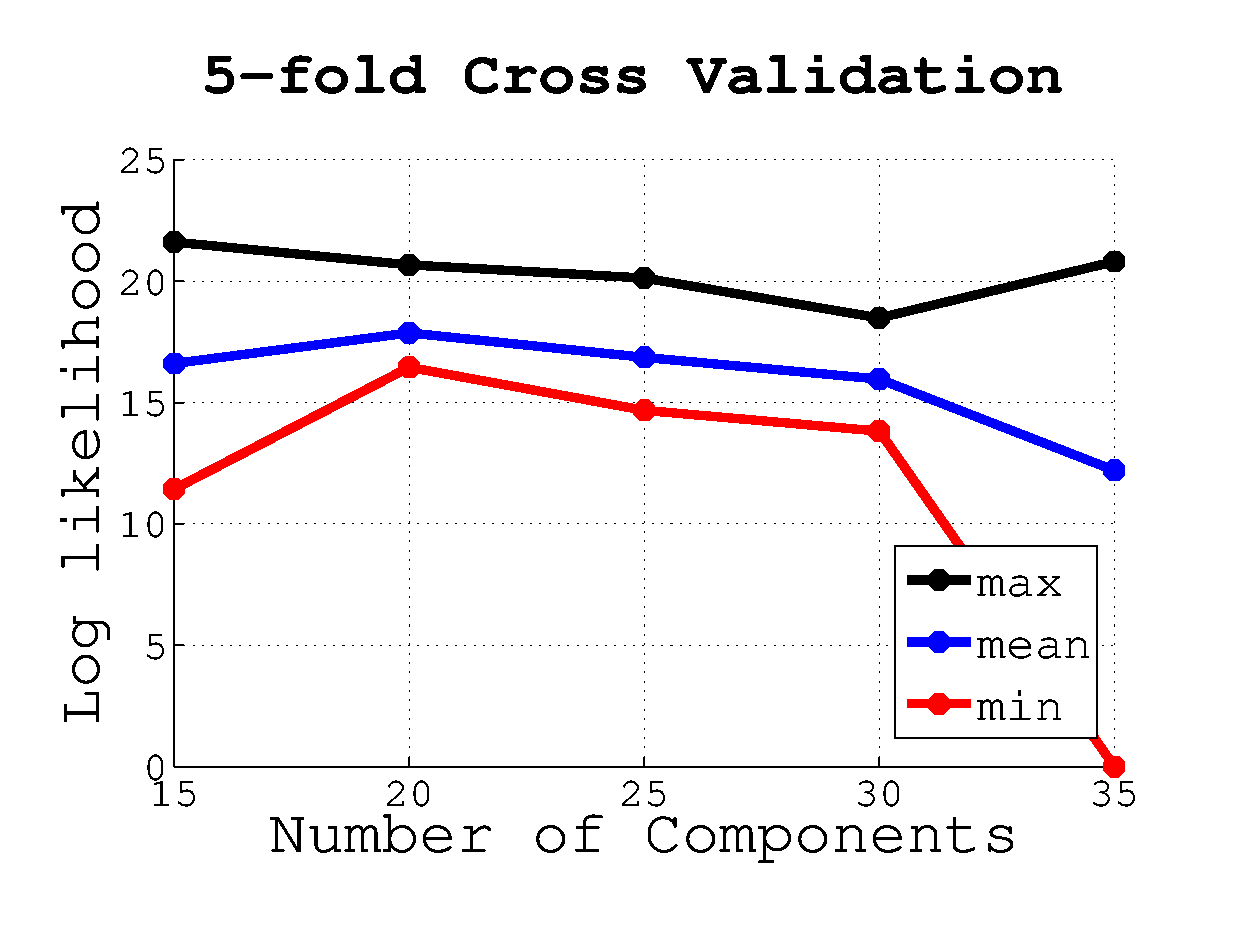
\includegraphics[width=7cm]{./fig_cha3/xValidation.eps}}

  \caption{\scriptsize{The $Bayesian$ $Information$ $Criterion$ and 5-fold cross validation test results of the training dataset of the Barrett hand and a joystick shaped object. For each number of Gaussians, the test is run 5 times. After empirical testing, the number of Gaussians is chosen to be 20. The corresponding experiment are shown in Section~\ref{cha3:sec3}.}
}
    \label{bicxv}
\end{figure}

\subsection{Grasp Planning}
\label{cha3:sec2:plangrasp}

With the learned GMM model of the grasping demonstrations, we plan a feasible grasp given a current hand configuration \textbf{\emph{q}}=\{\textbf{\emph{h}},\textbf{\emph{o}}\}. As discussed above, we first need to determine whether the \textbf{\emph{q}} is a valid query point. To do this we define a membership function $f$(\textbf{\emph{q}}) as:

\begin{equation}
f(\boldsymbol{q}) = \sum_{k=1}^{K}\bar{\boldsymbol{N}}(\boldsymbol{q};\boldsymbol{\mu}_k,\boldsymbol{\Sigma}_k)
\end{equation}
where $\bar{\boldsymbol{N}}$ is the normal distribution with the output being normalized between 0 and 1:

\begin{equation}
\bar{\boldsymbol{N}}(\boldsymbol{q};\boldsymbol{\mu}_k,\boldsymbol{\Sigma}_k) = exp\left(-\frac{1}{2}(\boldsymbol{q}-\boldsymbol{\mu}_k)^{T}\boldsymbol{\Sigma}_k^{-1}(\boldsymbol{q}-\boldsymbol{\mu}_k)\right)
\end{equation}

We consider a point to belong to the model if its Mahalanobis distance to any Gaussian component is less than a given threshold $\sigma$. In our experiments, we find that within 1~standard deviation the success rate of finding a feasible grasp is constantly high. For example in the Barrett hand and the model plane grasping task, the rate of producing a feasible and stable grasp within 1 standard deviation is 85\% (Table~\ref{result}) while it is 64\% within 3 standard deviations. On the other hand, it is possible that GMM encapsulates two different clusters of data within a single Gaussian, leaving the mean of the Gaussian at an infeasible point. This means getting closer to the means does not ensure a higher success rate. Taking this trade-off into account, we choose 1 standard deviation as our threshold, which gives us a cutoff criterion $\eta$ = $exp(-\frac{1}{2}\sigma^2)$. If the membership function of a point has a higher value than $\eta$, we consider this point as a valid query point. Note that the finger configuration $\boldsymbol\theta$ is not part of this input query point as $\boldsymbol\theta$ will be inferred by GMR later.

This membership function differs from the marginal likelihood $p$(\textbf{\emph{h}},\textbf{\emph{o}}) in two aspects. Firstly, it gives each Gaussian component the same weight, regardless of their priors $p_k$. As the prior of each Gaussian is proportional to the number of data points that are explained by this Gaussian, using this information in our selection may bias our choice toward the ``most popular" grasps, yielding less variety in the results.
Secondly, $\bar{\boldsymbol{N}}$ is a normalized function bounded between 0 and 1. This ensures the points with the same Mahalanobis distance from a Gaussian will have the same membership value, regardless of the size of the covariance~\citep{sauser2011iterative}.


In the case that \textbf{\emph{q}} is not a valid query point, we need to project it to a new point $\boldsymbol{q}^*$ that has a membership function value higher than $\eta$. Here we use a closed-form solution by considering each individual Gaussian component. We first compare the Mahalanobis distances between the query point \textbf{\emph{q}} and each Gaussian to find the nearest Gaussian component. The projection point $\boldsymbol{q}^*$ is found by projecting $\boldsymbol{q}$ to this nearest component (Figure~\ref{contour}).
%Point \textbf{\emph{q}} is then projected to this component to find the nearest point $\boldsymbol{q}^*$, which is less than one standard deviation away from the center of the Gaussian (Figure~\ref{contour}).
In the Mahalanobis space the Gaussian is in a uniform shape. As a result, the projection point $\boldsymbol{q}^*$  lays on the direction from the \textbf{\emph{q}} to the center of the Gaussian. Therefore the projection point $\boldsymbol{q}^*_k$ of the $k^{th}$ Gaussian can be written as:


\begin{equation}
\boldsymbol{q}^*_k = \boldsymbol{q} + \alpha_k(\boldsymbol{q}-\boldsymbol{\mu}_k)
\end{equation}
where $\alpha_k$ is a scalar. With $\sigma = 1$ and the equation

\begin{equation}
\bar{\boldsymbol{N}}_k(\boldsymbol{q};\boldsymbol{\mu}_k,\boldsymbol{\Sigma}_k) = exp(-\frac{1}{2}\sigma^2)
\end{equation}
we have the equation to easily compute $\boldsymbol{q}^*_k$:

\begin{equation}
-\frac{1}{2}(\boldsymbol{q}^*_k-\boldsymbol{\mu}_k)^{T}\boldsymbol{\Sigma}^{-1}_{k}(\boldsymbol{q}^*_k-\boldsymbol{\mu}_k) = -\frac{1}{2}\cdot{1}^{2}
\end{equation}

Once the projection point $\boldsymbol{q}^*$ is found, the $Gaussian$ $Mixture$ $Regression$ (GMR) is used to predict a feasible finger configuration $\boldsymbol\theta^*$ for it. First we define:

\begin{equation}
{
\boldsymbol{\mu}_{q,k} = \begin{pmatrix} \boldsymbol{\mu}_{h,k}    \\
                                        \boldsymbol{\mu}_{o,k}
                        \end{pmatrix}
\hspace{0.3in}
\boldsymbol{\Sigma}_{qq,k} =  \begin{pmatrix}  \boldsymbol{\Sigma}_{hh,k}  & \boldsymbol{\Sigma}_{ho,k}  \\
                                            \boldsymbol{\Sigma}_{oh,k}  & \boldsymbol{\Sigma}_{oo,k}
                            \end{pmatrix}
}
\end{equation}
and GMR then uses:

\begin{equation}
{
\hat{\boldsymbol{\mu}}_{\theta,k} = \boldsymbol{\mu}_{\theta,k} + \boldsymbol{\Sigma}_{\theta{q},k}(\boldsymbol{\Sigma}_{qq,k})^{-1}(\boldsymbol{q}-\boldsymbol{\mu}_{q,k})
}
\end{equation}

\begin{equation}
{
\hat{\boldsymbol{\Sigma}}_{\theta\theta,k} = \boldsymbol{\Sigma}_{\theta\theta,k} - \boldsymbol{\Sigma}_{\theta{q},k}(\boldsymbol{\Sigma}_{qq,k})^{-1}\boldsymbol{\Sigma}_{{q}\theta,k}
}
\end{equation}


Finally, all the $K$ components are taken into account and the target finger configuration $\boldsymbol{\theta}^*$ is predicted as the mean $\hat{\boldsymbol{\mu}}_\theta$ with the covariance $\hat{\boldsymbol{\Sigma}}_{\theta\theta}$ according to:

\begin{equation}
{
\hat{\boldsymbol{\mu}}_{\theta} = \sum_{k=1}^K{\beta_k(\boldsymbol{q}^*)}\hat{\boldsymbol{\mu}}_{\theta,k}
}
\end{equation}
\begin{equation}
{
\hat{\boldsymbol{\Sigma}}_{\theta\theta} = \sum_{k=1}^K{\beta_k(\boldsymbol{q}^*)}^2\hat{\boldsymbol{\Sigma}}_{\theta\theta,k}
}
\end{equation}
where
\begin{equation}
{
\beta_k(\boldsymbol{q}^*) = \frac{p_{k}p(\boldsymbol{q}^*|\boldsymbol{\mu}_{q,k},\boldsymbol{\Sigma}_{qq,k})}{\sum_{k=1}^K{p_k}p(\boldsymbol{q}^*|\boldsymbol{\mu}_{q,k},\boldsymbol{\Sigma}_{qq,k})}
}
\end{equation}

Due to the probabilistic nature of the GMR, the inferred result $\boldsymbol{\theta}^*$ is not a unique value but a mean value with variance. Though this mean does not guarantee a feasible solution, it provides a good estimation of a feasible one.

To find the closest Gaussian component we used the Mahalanobis distance rather than the Euclidean distance. The advantage of this is that it takes into account the correlations among each dimension of the hand configuration. In a space of different types of measurements, i.e. length and angle, Mahalanobis space is a better representation than the Euclidean space. Indeed, humans do not always use the Euclidean distance to select their grasps. We may move our hand further than needed to grasp an object, in order to avoid flipping our hand to another orientation. The performance of this method is discussed in the next section.


\section{Experiments of planning grasps for familiar objects}
\label{cha3:sec3}

This section presents a few results of our method (Figure~\ref{contour},~\ref{icub_cuboid}\footnote{The small penetrations and gaps between the fingers and the object are caused by two factors, (1) that the width of the fingers are not taken into account in the optimization and (2) the variance of the results. A supplemental implementation will be applied on the real scenario to handle the variances.},~\ref{barrett}). As mentioned above, grasps of the iCub hand are described in 14 dimensions: hand position (3D), hand orientation (3D in Euler angles) and finger joint angles (8D). Grasps of the Barrett hand are described in 8 dimensions: hand position (3D), hand orientation (4D in axis-angle representations) and finger separation angle (1D). Six different objects are presented here: cylinder, cuboid, ashtray, shoe, joystick and aeroplane model. For each object, three different initial postures and their final grasps are shown. Figure~\ref{contour} shows the results of the iCub grasping a cylinder, and the corresponding projections from the initial query points to the model. The results of the cylinder and cuboid show that a variety of grasps can be obtained for simple shapes to satisfy different task requirements. The ashtray, aeroplane model and joystick shapes are chosen from the GraspIt! object library, showing the method indeed works with complex shapes. In some figures the wrist may seem to rotate over 360 degrees to reach the final grasps from the initial pose. This is because the path planning of the arm is not taken into account in our approach. In terms of the hand orientation solely, a much smaller rotation is needed to go from the initial pose to the final grasp.

\begin{figure}

  \centering
  \subfloat[\scriptsize{Initial pose 1}]  {\label{fig:reachableSamplesPos}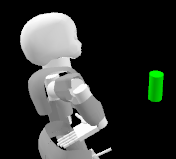
\includegraphics[width=4cm]{./fig_cha3/1_ini.png}}
  \subfloat[\scriptsize{Initial pose 2}] {\label{fig:reachableModelPos}  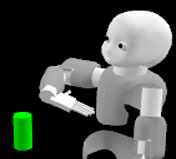
\includegraphics[width=4cm]{./fig_cha3/2_iniss.png}}
  \subfloat[\scriptsize{Initial pose 3}]  {\label{fig:reachableSamplesPos}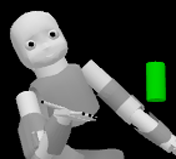
\includegraphics[width=4cm]{./fig_cha3/aa.png}}

  \vspace{0.02in}
  \subfloat[\scriptsize{Final grasp 1}] {\label{fig:reachableSamplesPos}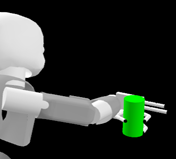
\includegraphics[width=4cm]{./fig_cha3/1_finalss.png}}
  \subfloat[\scriptsize{Final grasp 2}] {\label{fig:reachableModelPos}  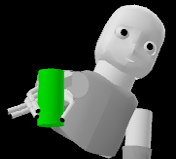
\includegraphics[width=4cm]{./fig_cha3/2_finalss.png}}
  \subfloat[\scriptsize{Final grasp 3}]  {\label{fig:reachableSamplesPos}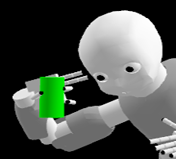
\includegraphics[width=4cm]{./fig_cha3/3_final_2ss.png}}

  \vspace{0.2in}
  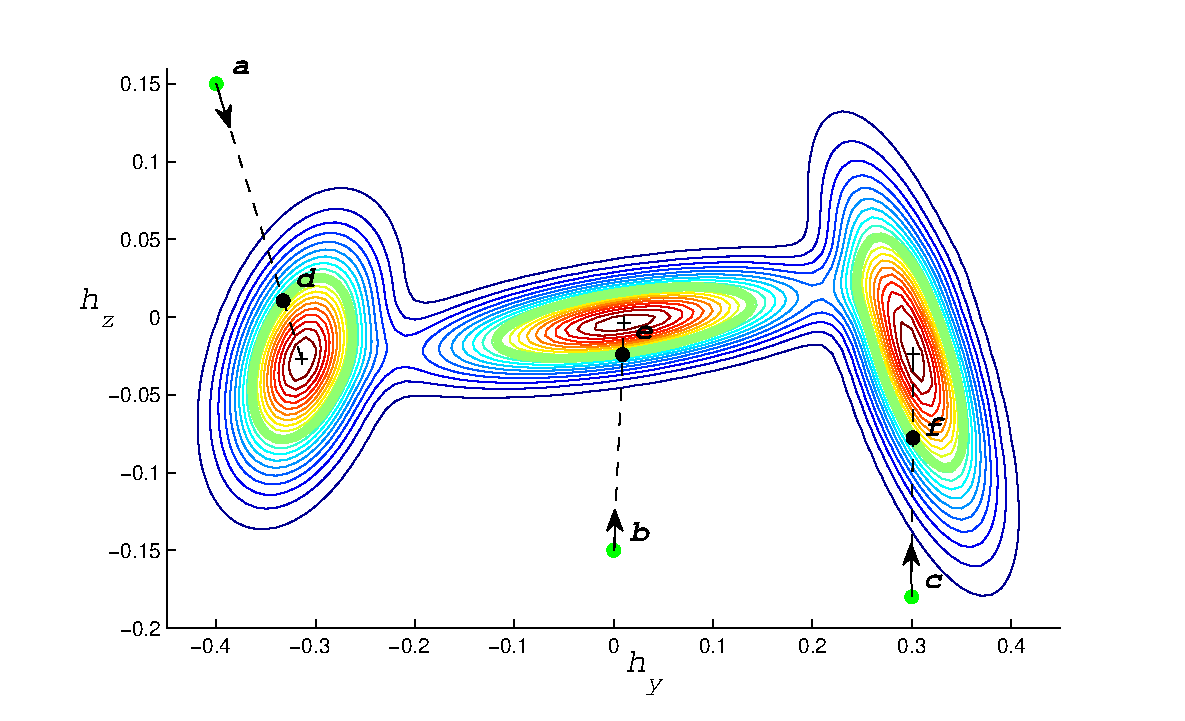
\includegraphics[width=14cm]{./fig_cha3/contour2-3_4.eps}
  \caption{\scriptsize{
  Two-dimensional illustration of the learned model. $h_y$ and $h_z$ correspond to the hand position along the y and z axis of the object reference frame. a, b and c are the initial query points, while d, e and f are their corresponding computed grasps.
  Green dots correspond to initial query inputs  {\bf {\em q}}, black dots correspond to found feasible query inputs {\bf {\em q}}$^*$, contours correspond to parts of the space with constant likelihood, and the thick green contours correspond to threshold values $\eta$ = exp(-$\frac{1}{2}\sigma^2$) of each Gaussian, where $\sigma = 1$ standard deviations.
  The initial finger joint angles in a,b,c are all set to zero. After each feasible query point is found, GMR is used to predict the finger configuration to get the final grasp d,e,f. }
}
    \label{contour}
\end{figure}


\begin{figure}
  \centering
    \subfloat[\scriptsize{Initial pose 1}]  {\label{fig:reachableSamplesPos}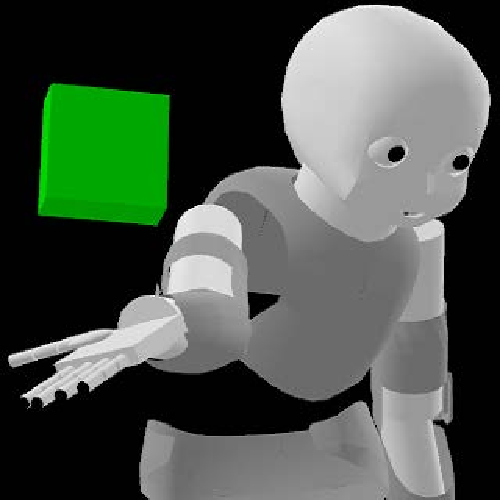
\includegraphics[width=5cm]{./fig_cha3/cuboid_1_i.pdf}}
    \subfloat[\scriptsize{Initial pose 2}] {\label{fig:reachableModelPos}  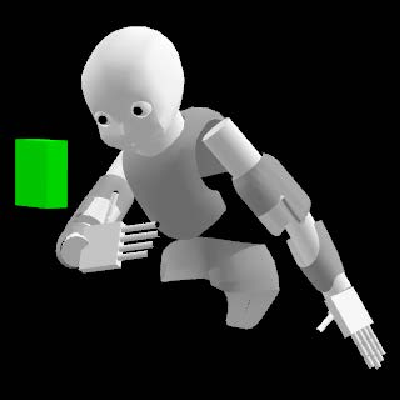
\includegraphics[width=5cm]{./fig_cha3/cuboid_2_i.pdf}}
    \subfloat[\scriptsize{Initial pose 3}] {\label{fig:reachableModelPos}  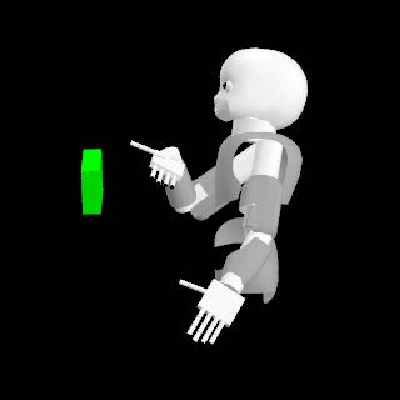
\includegraphics[width=5cm]{./fig_cha3/cuboid_3_i.pdf}}

    %\vspace{0.05in}

    \subfloat[\scriptsize{Final grasp 1}] {\label{fig:reachableModelPos}  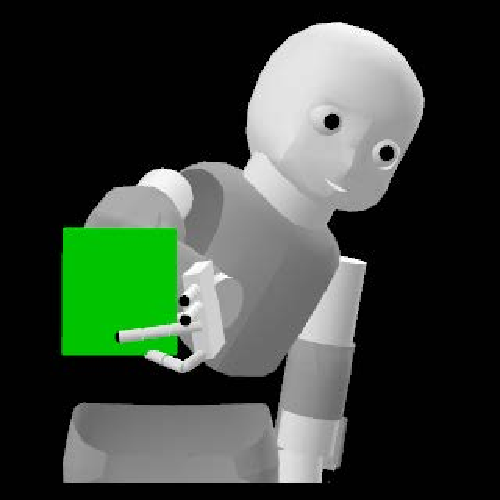
\includegraphics[width=5cm]{./fig_cha3/cuboid_1_f.pdf}}
    \subfloat[\scriptsize{Final grasp 2}]  {\label{fig:reachableSamplesPos}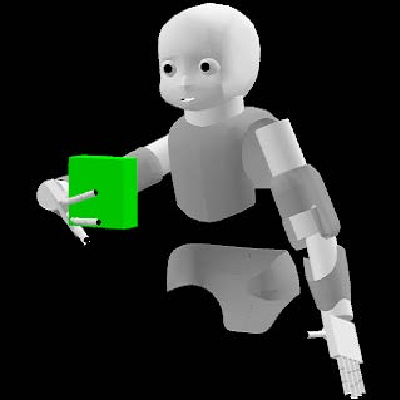
\includegraphics[width=5cm]{./fig_cha3/cuboid_2_f.pdf}}
    \subfloat[\scriptsize{Final grasp 3}]  {\label{fig:reachableSamplesPos}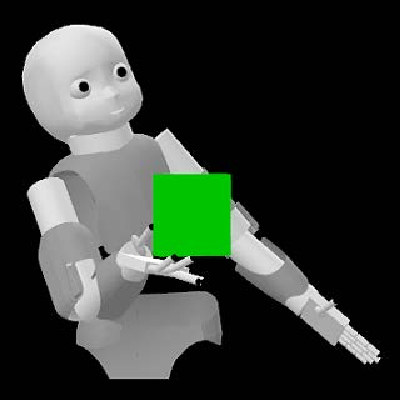
\includegraphics[width=5cm]{./fig_cha3/cuboid_3_f.pdf}}

  \caption{\scriptsize{Examples of the iCub hand grasping a cuboid. The first row (a,b,c) shows the initial postures and the second row (d,e,f) shows the corresponding final grasps.}
}
    \label{icub_cuboid}
\end{figure}

To test the computation time we generated 3000 random initial query points for each grasping task. The initial query points are placed at different distances away from the object surface, varying between 3$cm$ to 50$cm$, and the hand orientation is random. The initial finger configuration is not taken into account in finding the feasible region and hence it is set to the robot hand starting values. The computation time and experimental details are shown in Table~\ref{result}. The computation is done by Matlab on a machine with a 2.8GHz processor and a 4GB RAM.

Table~\ref{result} also shows the success rate of generated grasps with the iCub and the Barrett hand. A grasp is considered to be successful if it satisfies the force-closure criterion, is feasible for the hand kinematics and is not in collision with the object (see Section~\ref{cha3:sec2:demonstration}). When executing the obtained grasp, the fingers will continue to clutch until contact is made; if they contact the object surface before reaching the expected finger configuration, they will halt to avoid penetration.
All the results shown in Figure.~\ref{contour},~\ref{icub_cuboid},~\ref{barrett} are good grasps.

As can be seen from Table~\ref{result}, the success rate depends on the dimensions of the grasp space and the surface geometry of the target objects. Grasps in lower degrees of freedom (the Barrett hand) have higher success rates than those in higher degrees of freedom (the iCub hand). This suggests that the higher dimension grasp space is more complex than the lower dimension grasp space and needs more data to represent the full complexity. On the other hand, objects with smooth surfaces have a success rate around 90\%. Objects with a couple of prominences have success rates over 85\% as the configuration space of grasping is discontinuous. In the Barrett hand and aeroplane model task, the failed grasps are concentrated on two places: the thin edges of the wings and the propeller. Grasping these places requires high accuracy and more training data on these parts would be needed.
%On the other hand, objects with smooth surface have a high rate of success. Objects with a couple of prominence have success rate about 85\% as the configuration space of grasping is discontinue. In the Barrett hand and airplane model task, the failure grasps are concentrated on two places: the thin edges of the wings and the propeller. Grasping these two places require high accuracy and this is not the main concern of this paper.

To compare with the training data, we compute the grasp quality of the results with the same metrics we used in data generation. The mean of the grasp quality of the training set and the result set are similar, though the result set has a slightly higher value in most of cases. We are able to find some grasps of higher quality than all grasps in the training set (Figure~\ref{near}). This shows that GMM is able to model and generalize the high dimensional grasp space, especially for objects with smooth surfaces.

% For the iCub hand, 612 different feasible grasps of a cylindrical object are obtained by the optimization~\citep{sahar2012}. The learned GMM model has 40 Gaussian components, determined by BIC, and each Gaussian has 14 dimensions: hand position (3D), hand orientation (3D), finger joint angles (8D).



\begin{figure}
  \centering
   \subfloat[\scriptsize{Best grasp found}]  {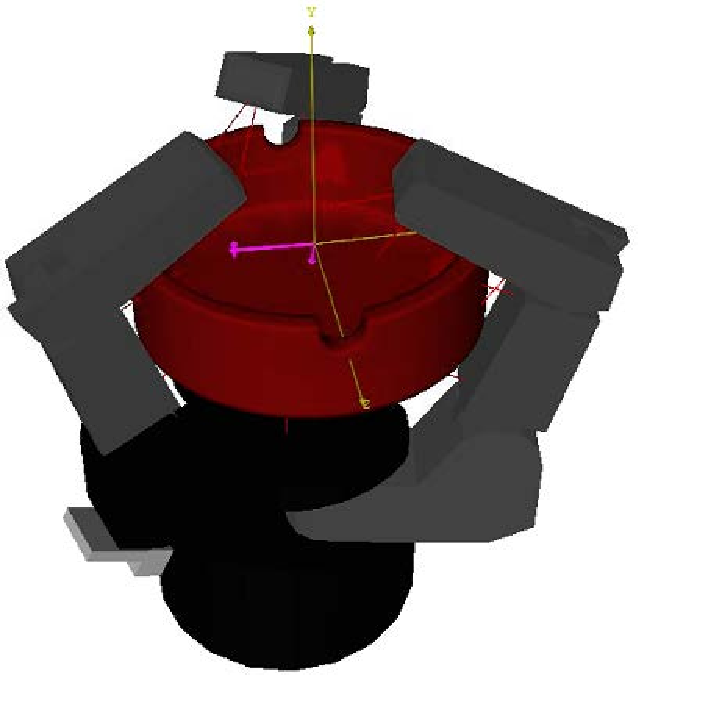
\includegraphics[width=3cm]{./fig_cha3/ash_near1.pdf}}
   \subfloat[\scriptsize{Neighbor grasp of (a)}] {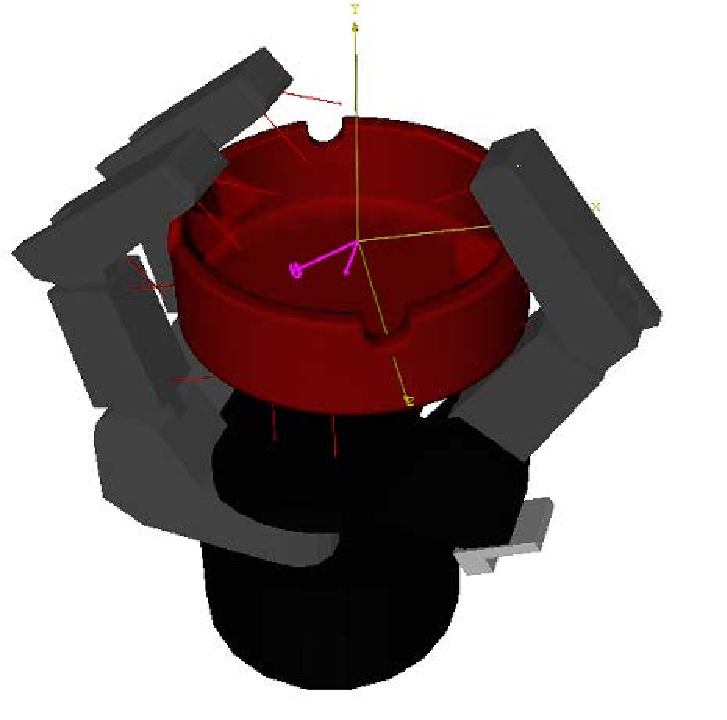
\includegraphics[width=3cm]{./fig_cha3/ash_near2.pdf}}
   \subfloat[\scriptsize{Best grasp found}] {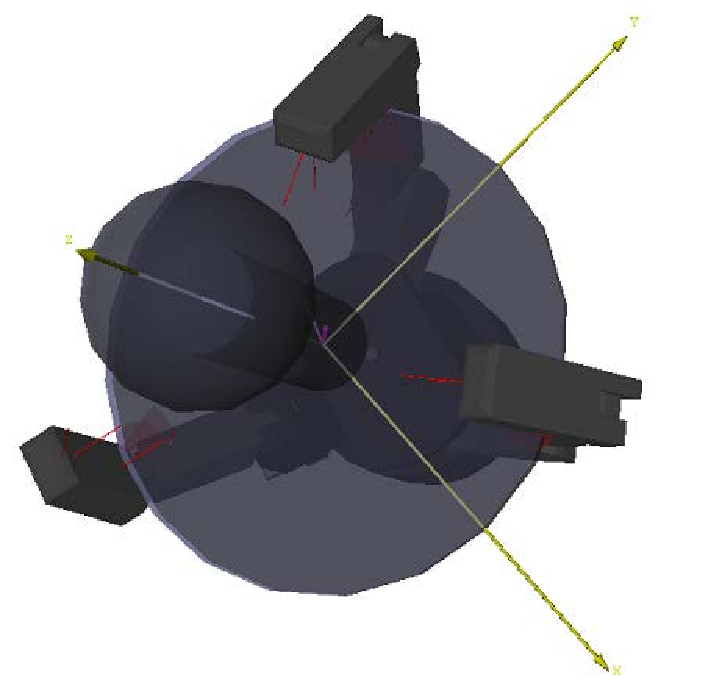
\includegraphics[width=3cm]{./fig_cha3/joy_near1.pdf}}
   \subfloat[\scriptsize{Neighbor grasp of (c)}] {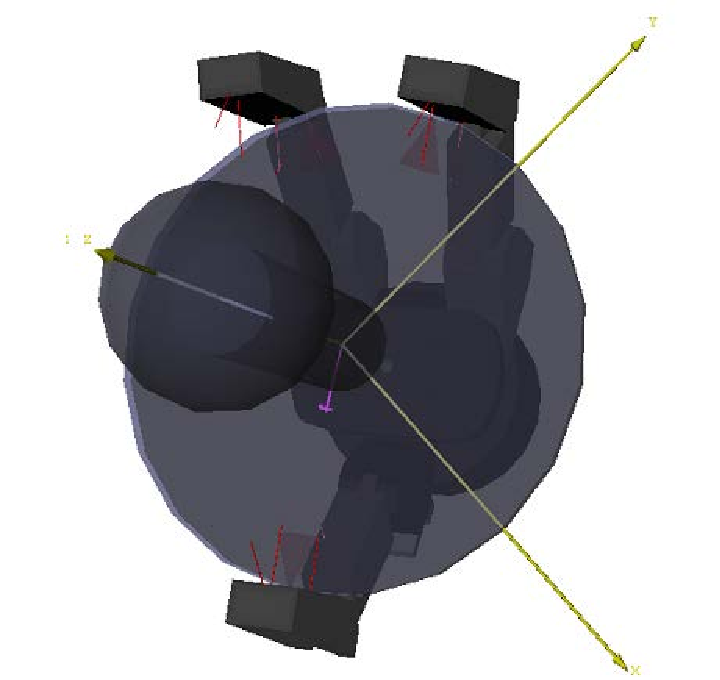
\includegraphics[width=3cm]{./fig_cha3/joy_near2.pdf}}

 \caption{\scriptsize{(a) The best grasp found for the Barrett hand and the ashtray. Grasp Quality is 0.16. (b) The nearest grasp of (a) in the training set. Note the gap between the finger and the object. Grasp Quality is 0.027. (c) The best grasp found for the Barrett hand and the joystick. Grasp Quality is 0.19. (d) The nearest grasp of (b) in the training set. Quality is 0.03 }
}
    \label{near}
\end{figure}


\begin{table*}
\renewcommand{\arraystretch}{1.5}
    \caption{Average computation time for generating new grasps for the iCub hand and the Barrett hand.}
    \hspace{-1.5cm}
    \begin{tabular}{|>{\centering\arraybackslash}p{3cm}|>{\centering\arraybackslash}p{1.2cm}|>{\centering\arraybackslash}p{1.7cm}|>{\centering\arraybackslash}p{1.2cm}|>{\centering\arraybackslash}p{1.5cm}|>{\centering\arraybackslash}p{1.5cm}|>{\centering\arraybackslash}p{1.7cm}|>{\centering\arraybackslash}p{1.7cm}|>{\centering\arraybackslash}p{0.9cm}|}%{ | c | c | c | c | c | c | c | c |p{1cm} |}
    \hline
    Robot/Object & Number of training data & Average Grasp Quality(train)& Number of Gaussians& Force-Closure Grasp Found & Average Grasp Quality(result)& Mean of Computation Time($msec$) & Variance ($msec$)   \\ \hline
    iCub/Cylinder       & 621   & 0.0965& 40    & 90\%  & 0.1008    & 9.1   & 0.0001 \\ \hline
    iCub/Cuboid         & 532   & 0.1317& 40    & 89\%  & 0.1224    & 9.4   & 0.0007 \\ \hline
    Barrett/Ashtray     & 1560  & 0.0975& 15    & 100\% & 0.1644    & 4.3   & 0.0001 \\ \hline
    Barrett/Shoe        & 629   & 0.0019& 25    & 99\%  & 0.0034    & 6.9   & 0.0001 \\ \hline
    Barrett/Joystick    & 1500  & 0.0061& 20    & 98\%  & 0.0064    & 5.9   & 0.0002 \\ \hline
    Barrett/Plane       & 1374  & 0.0002& 55    & 85\%  & 0.0003    & 15.1  & 0.0003 \\ \hline

    \end{tabular}

    \label{result}

\end{table*}


\begin{figure*}
  \centering

    \subfloat[\scriptsize{Initial pose 1}]  {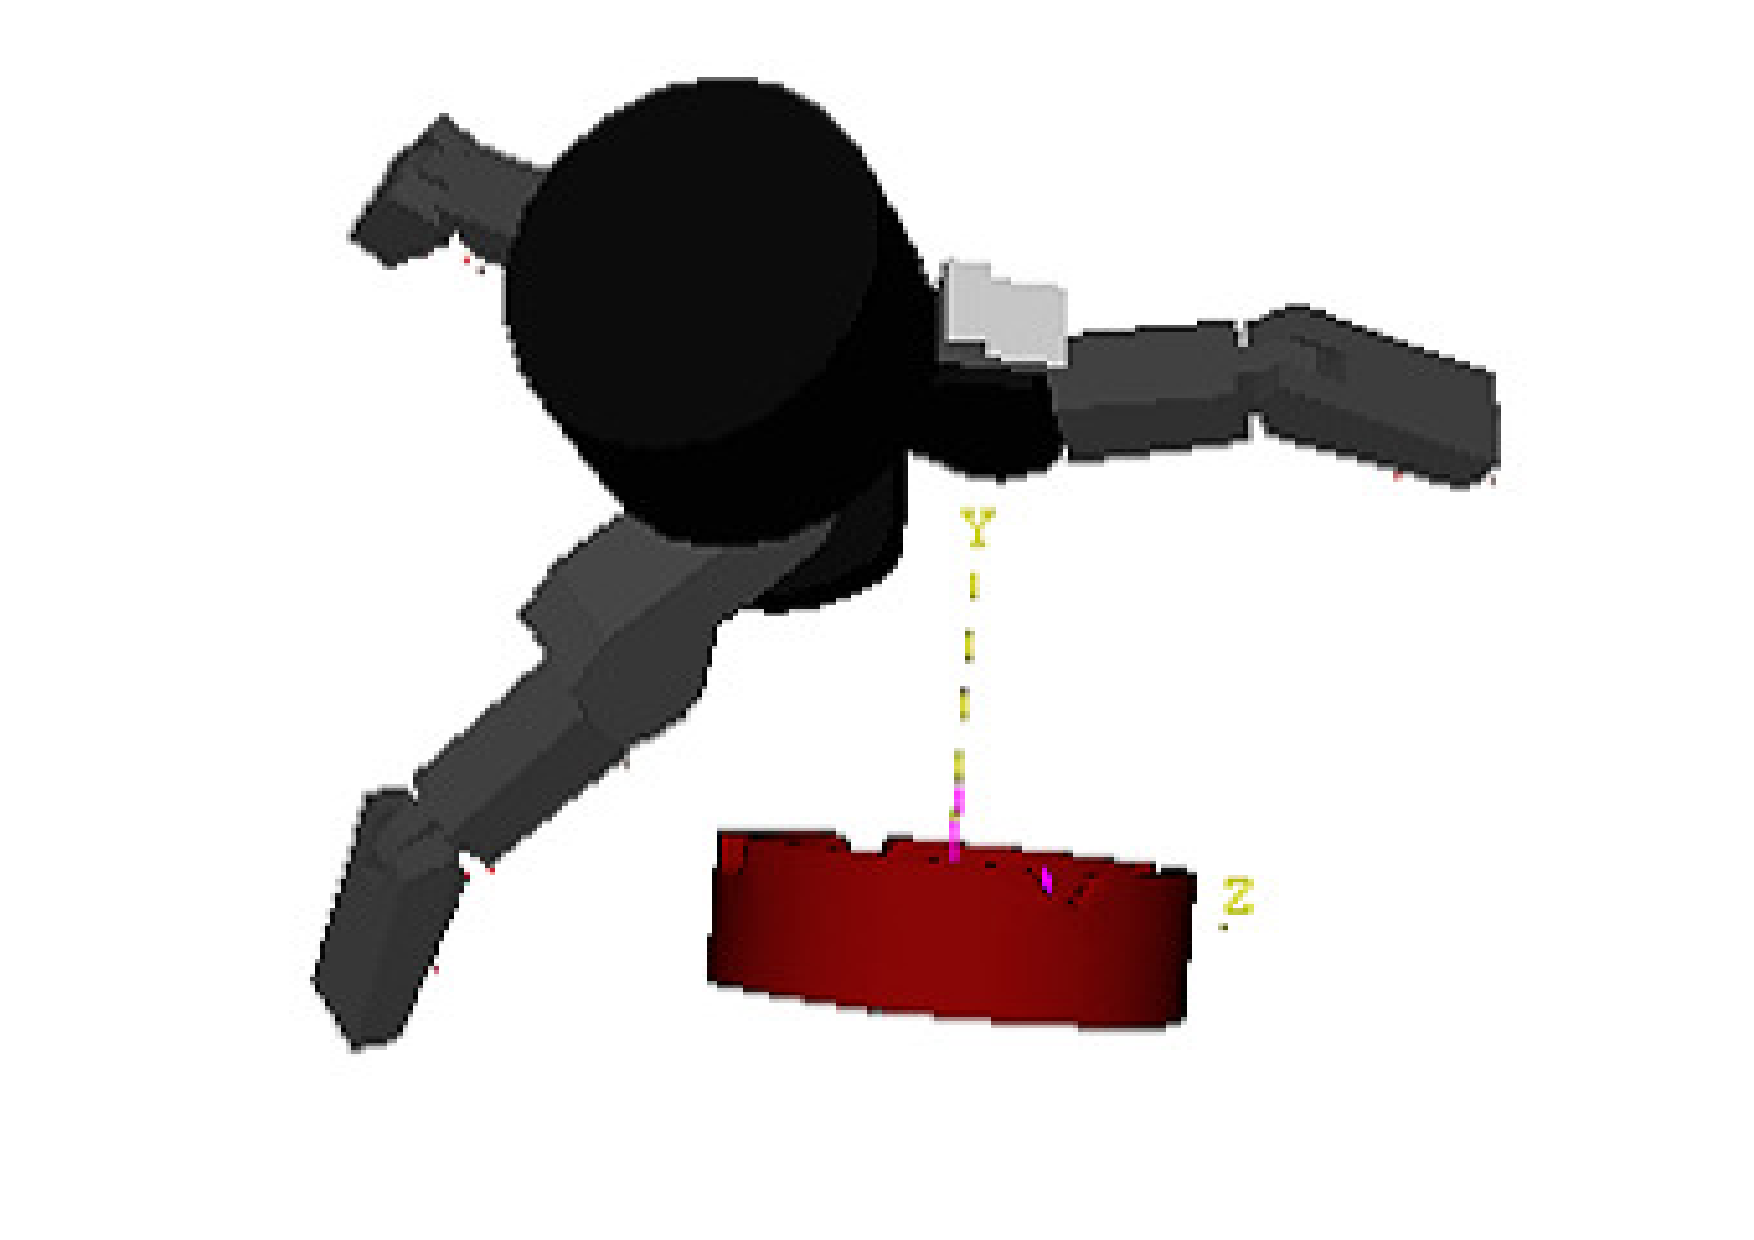
\includegraphics[width=4cm]{./fig_cha3/bar_i_1.pdf}}
    \subfloat[\scriptsize{Initial pose 2}] { 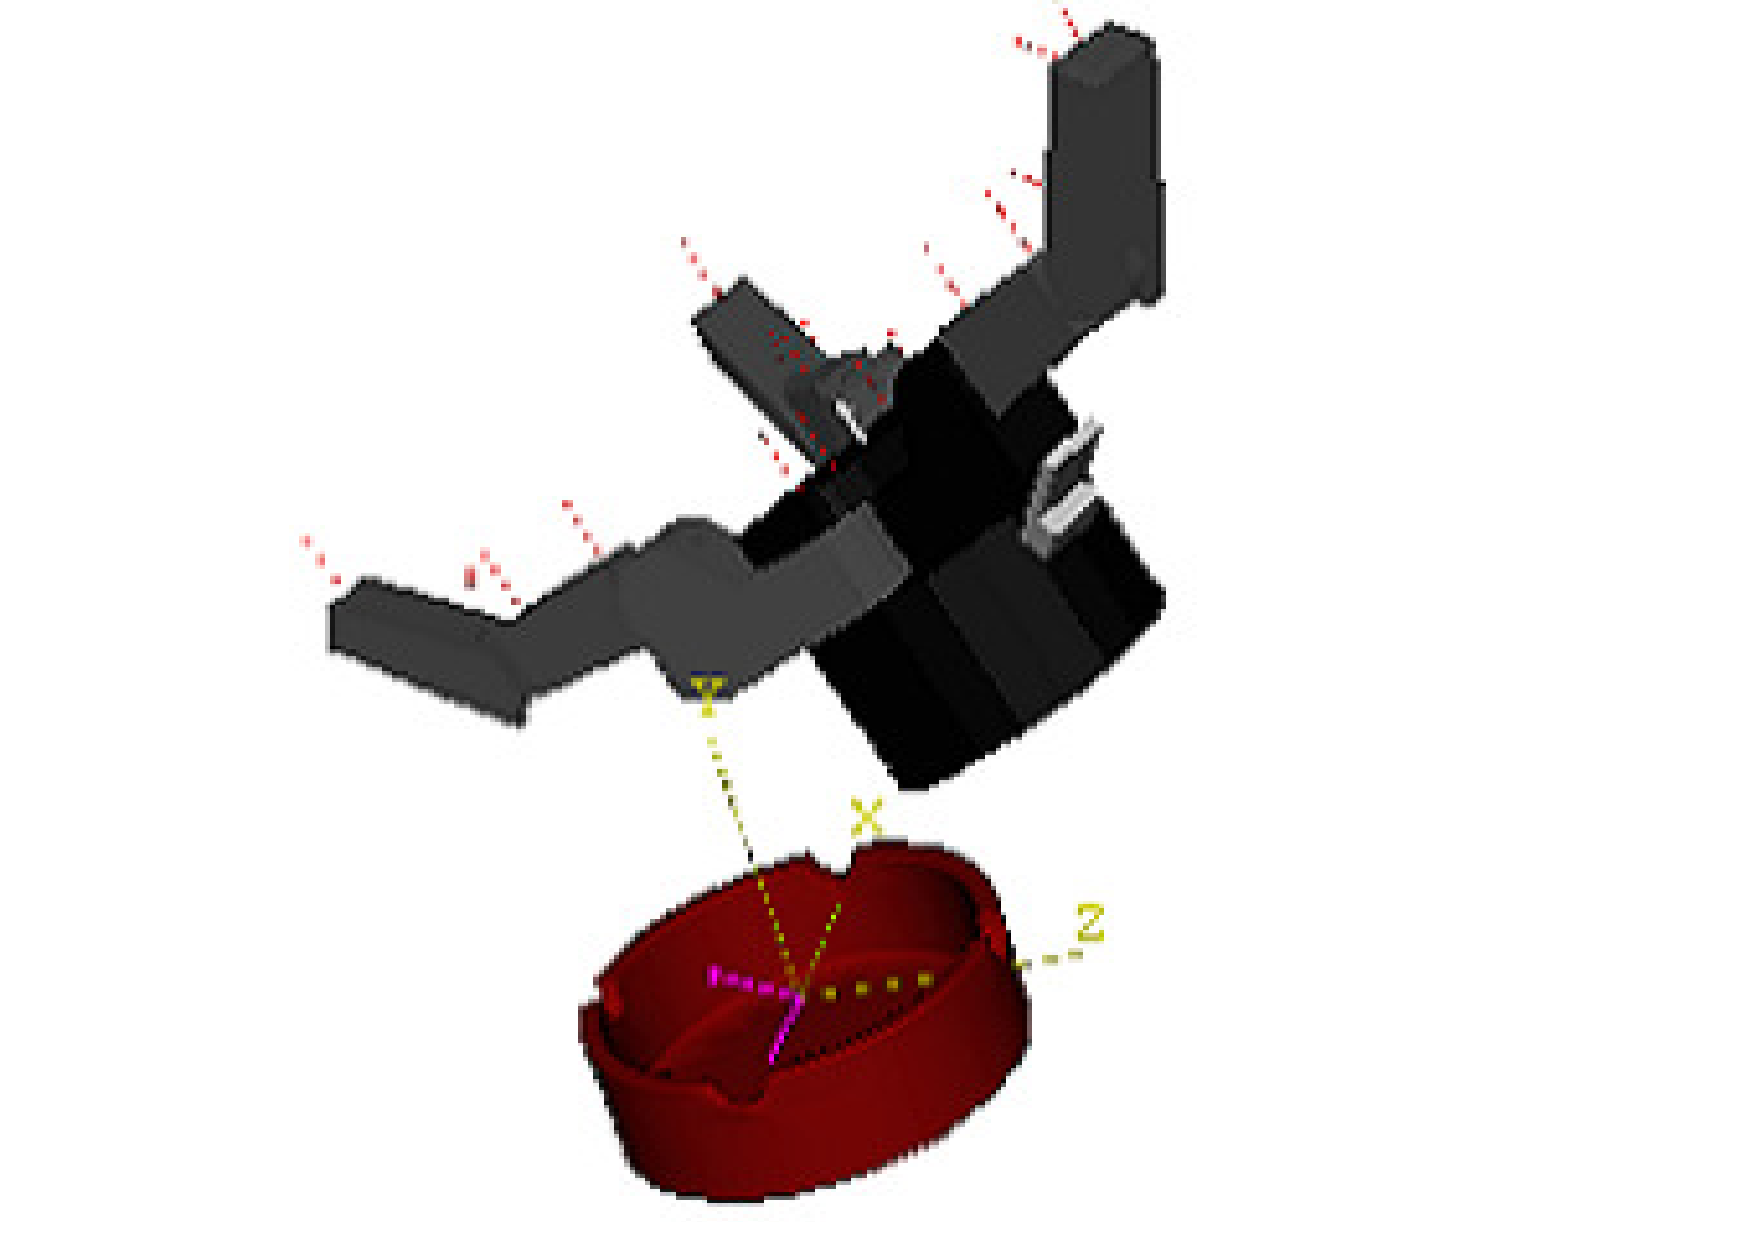
\includegraphics[width=4cm]{./fig_cha3/bar_i_2.pdf}}
    \subfloat[\scriptsize{Initial pose 3}] { 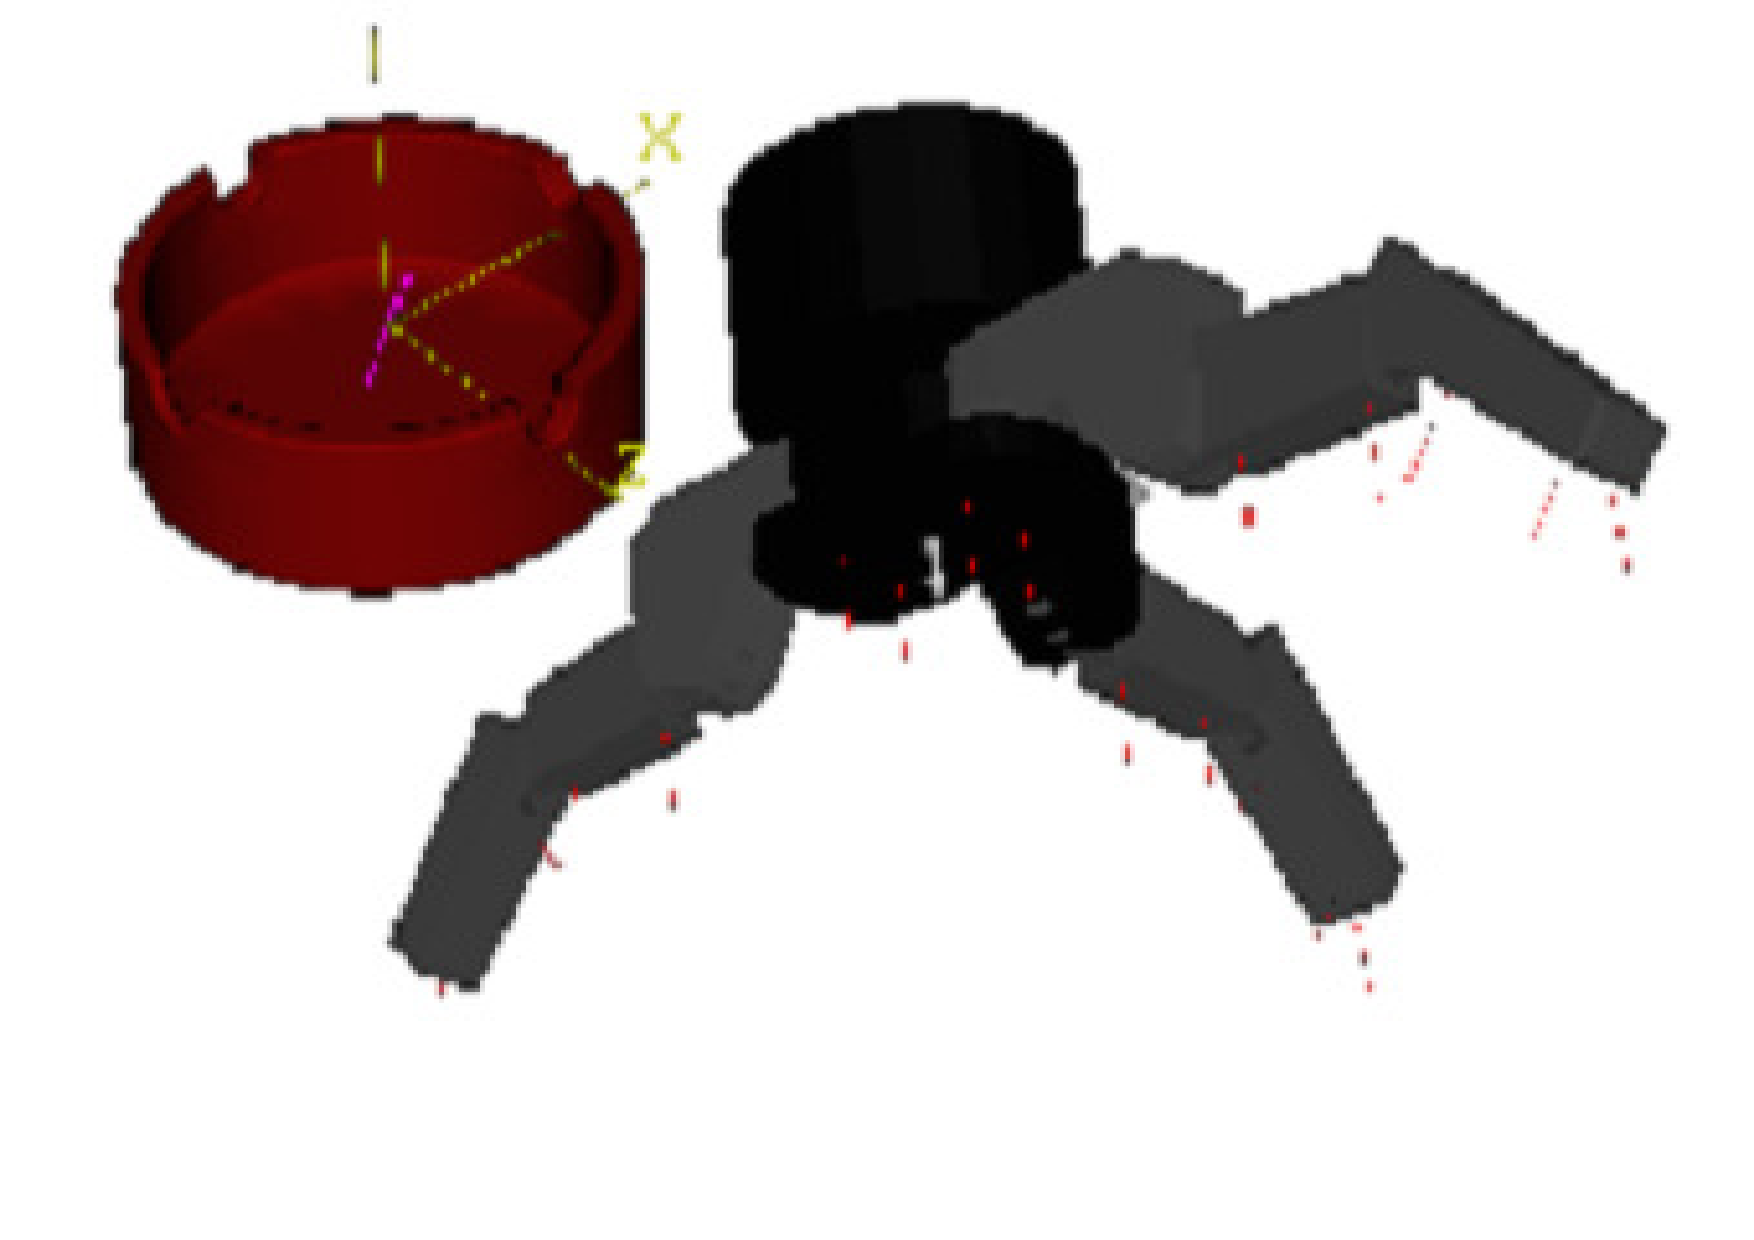
\includegraphics[width=4cm]{./fig_cha3/bar_i_3.pdf}}
    \vspace{0.3cm}
    \subfloat[\scriptsize{Final grasp 1}] {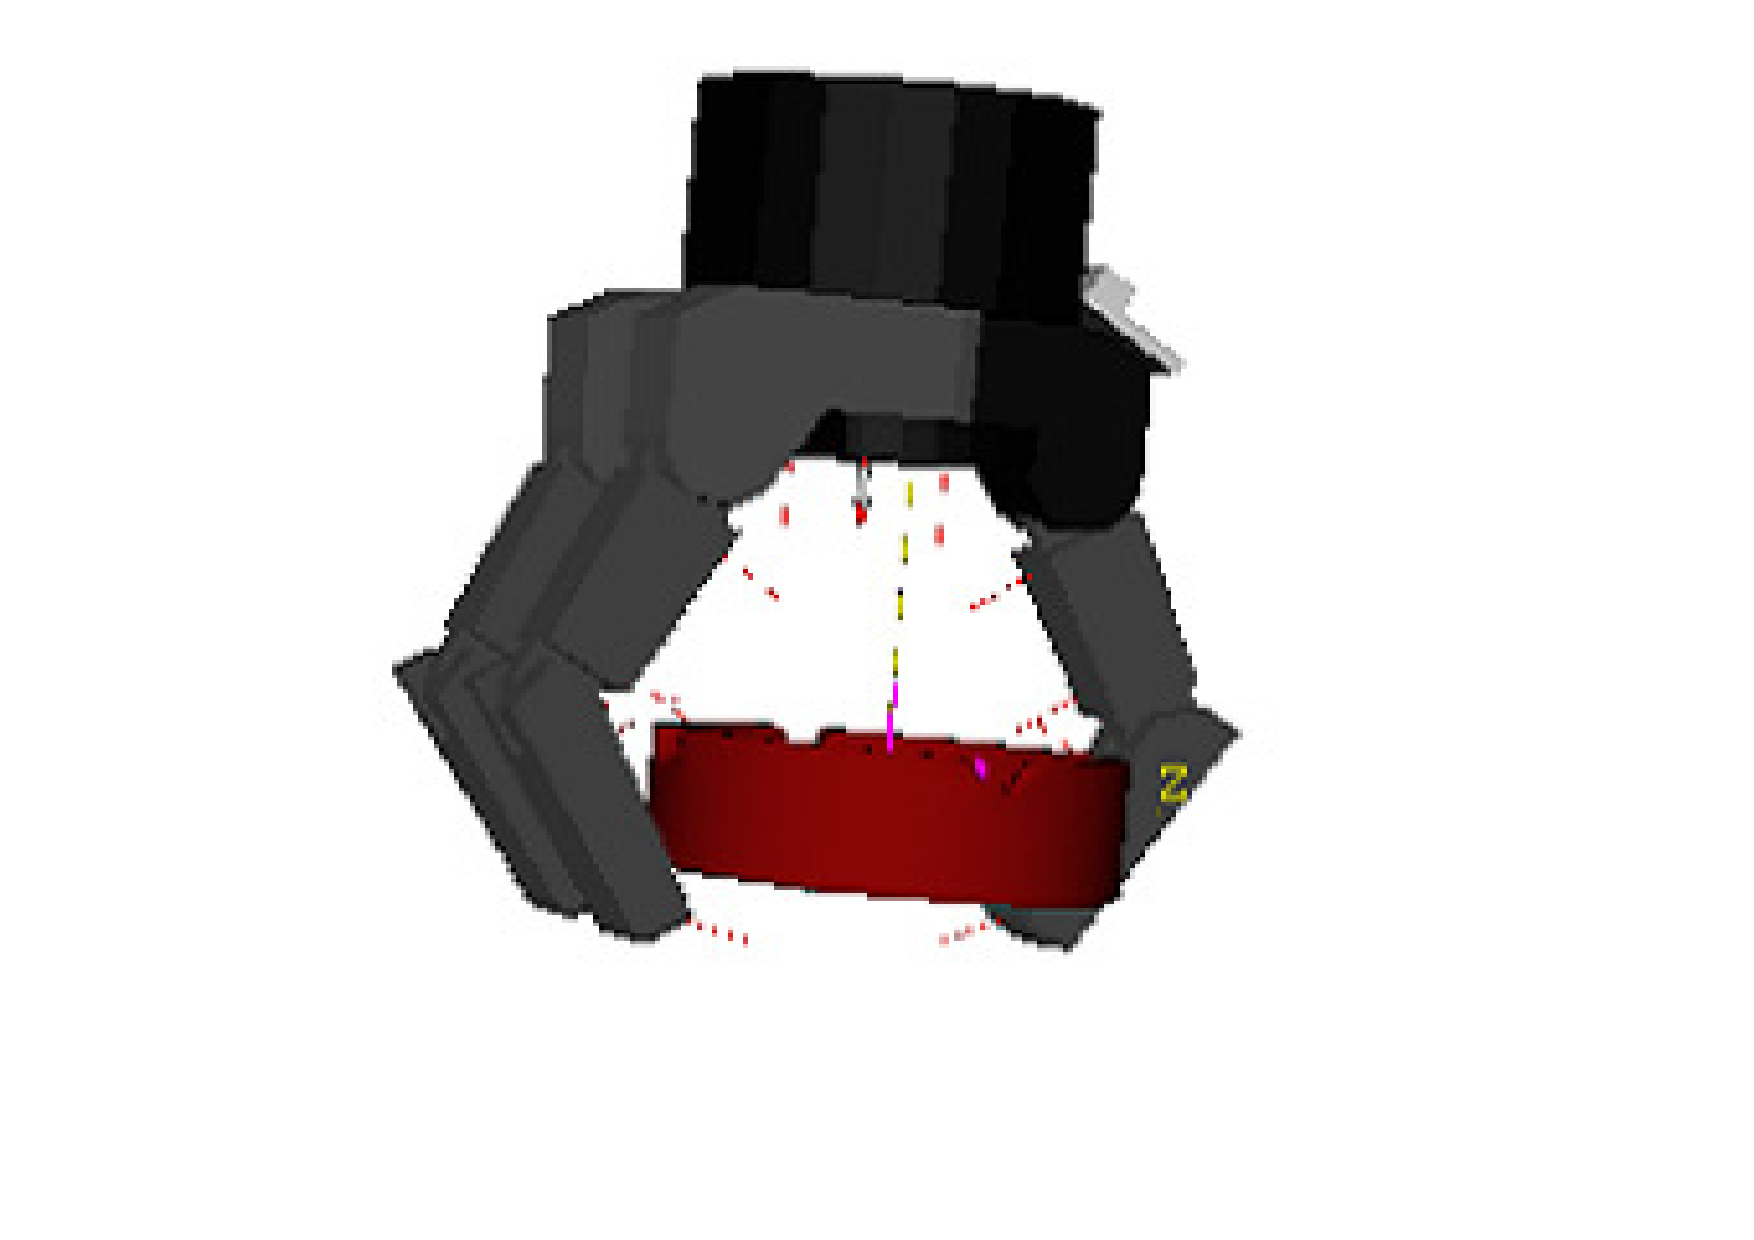
\includegraphics[width=4cm]{./fig_cha3/bar_f_1.pdf}}
    \subfloat[\scriptsize{Final grasp 2}]  {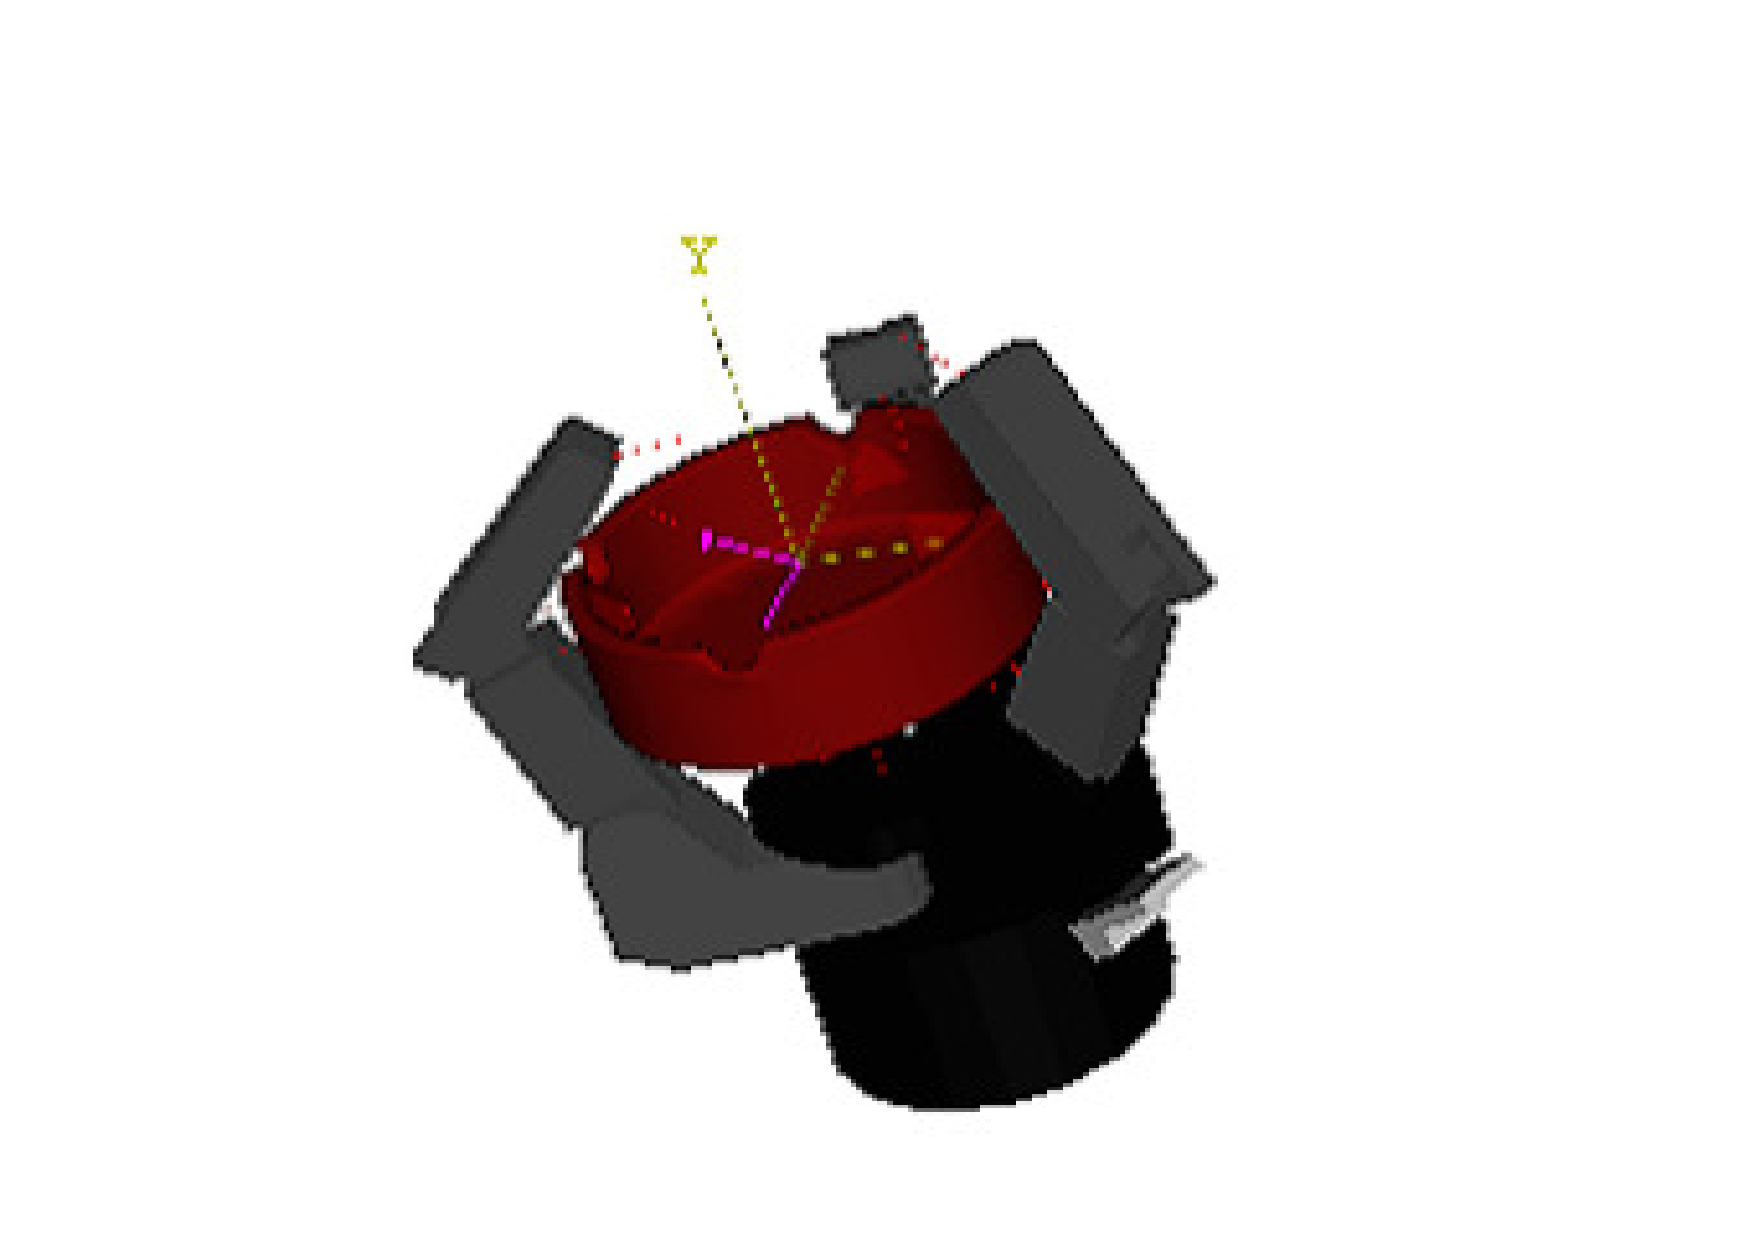
\includegraphics[width=4cm]{./fig_cha3/bar_f_2.pdf}}
    \subfloat[\scriptsize{Final grasp 3}]  {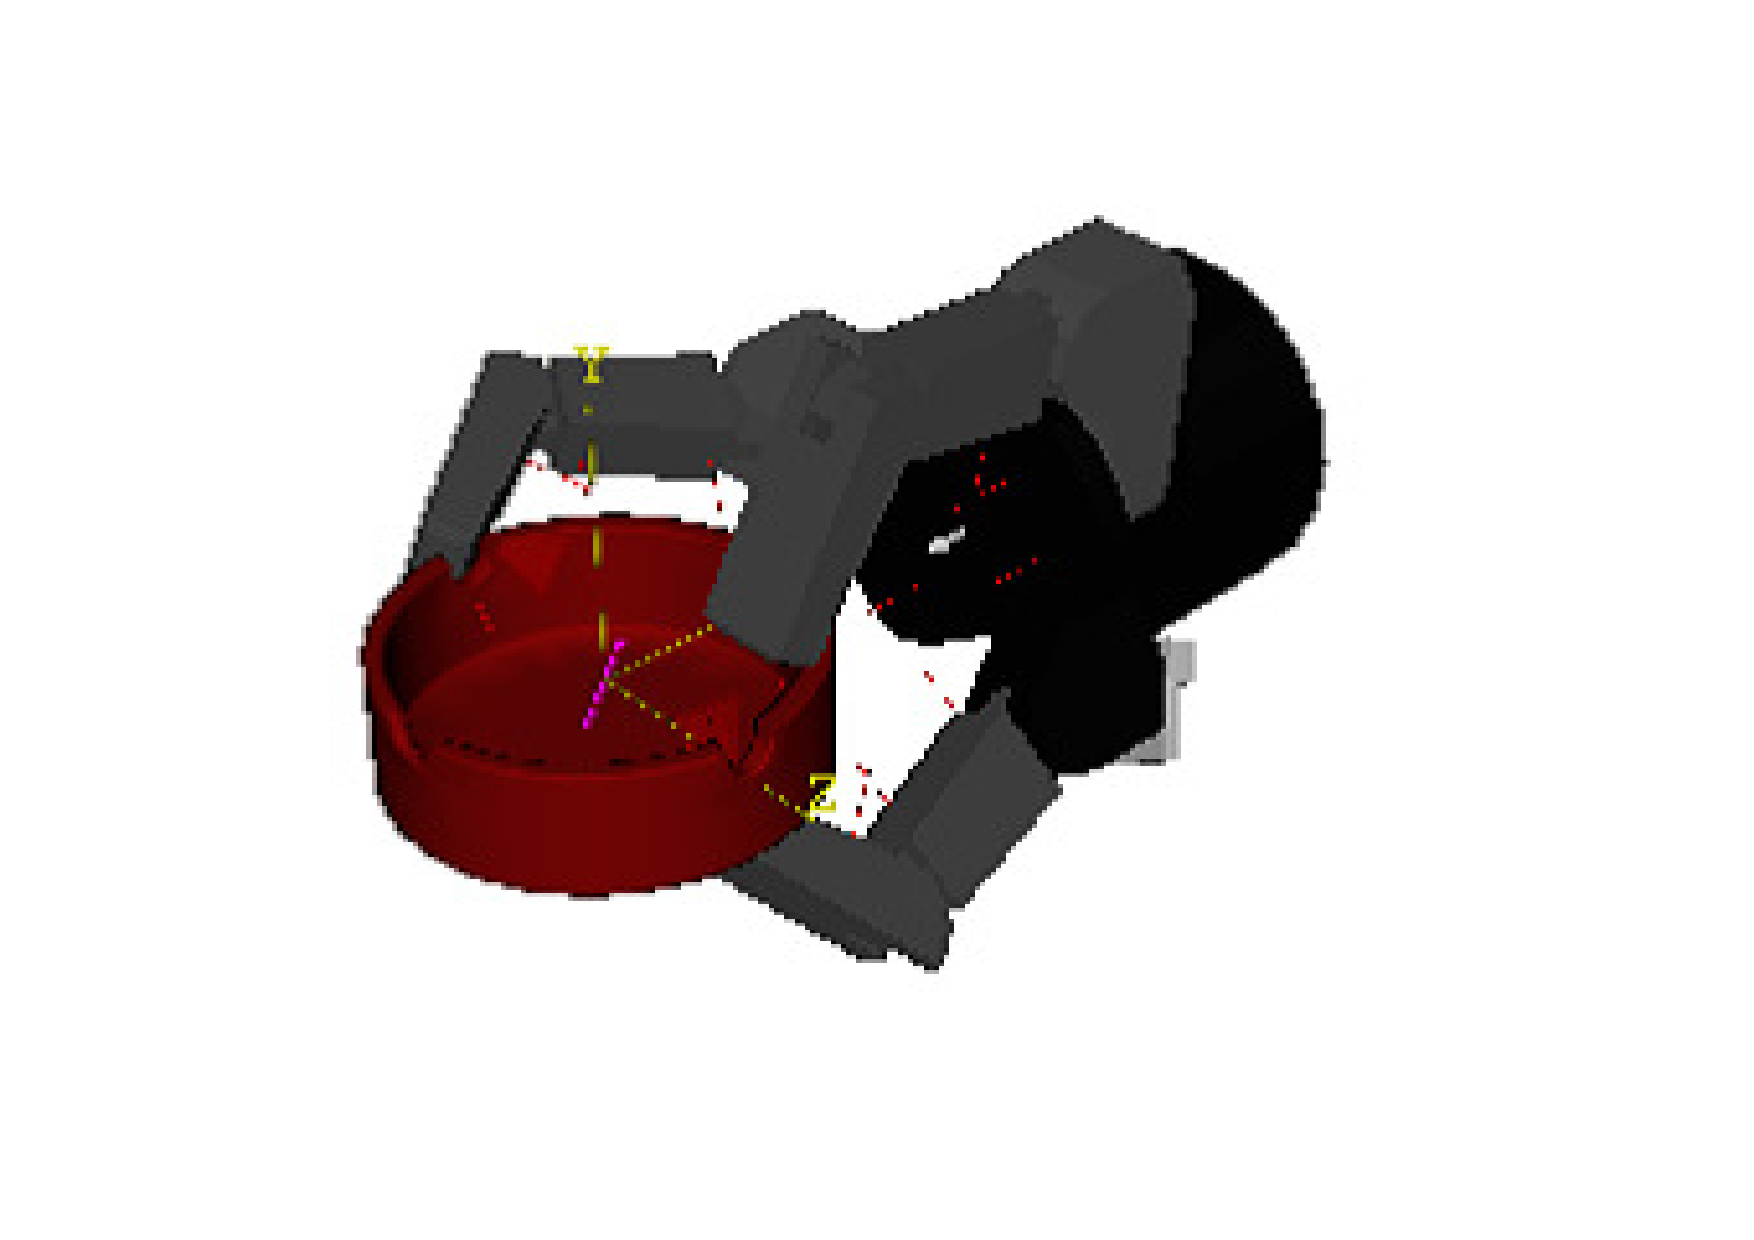
\includegraphics[width=4cm]{./fig_cha3/bar_f_3.pdf}}
    \vspace{0.3cm}
    \subfloat[\scriptsize{Initial pose 4}]  {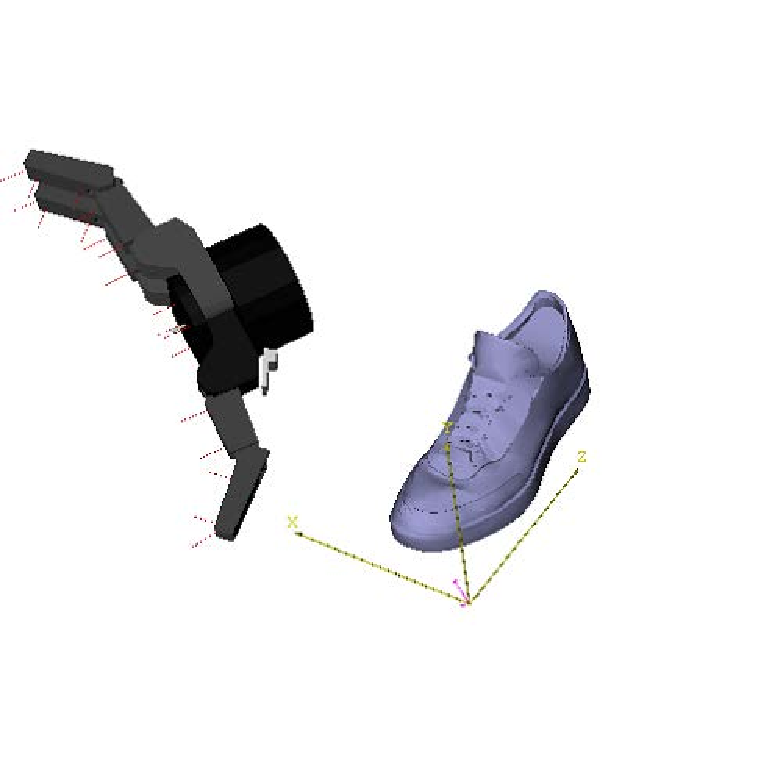
\includegraphics[width=4cm]{./fig_cha3/shoe_1i.pdf}}
    \subfloat[\scriptsize{Initial pose 5}] {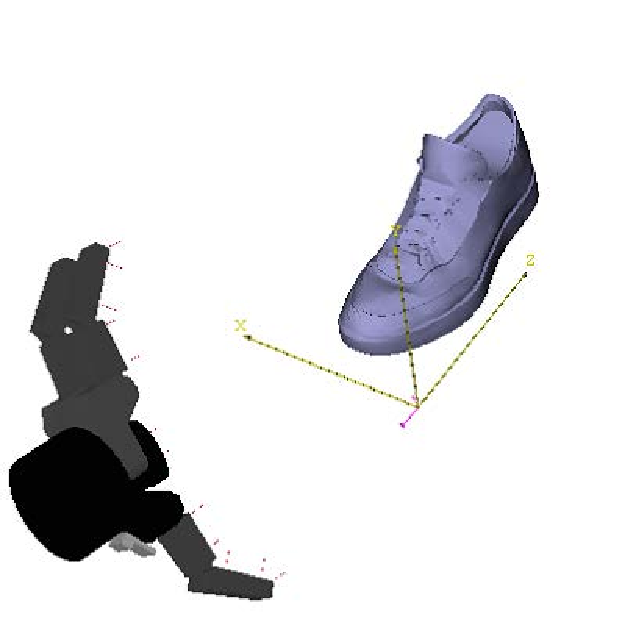
\includegraphics[width=4cm]{./fig_cha3/shoe_2i.pdf}}
    \subfloat[\scriptsize{Initial pose 6}]  {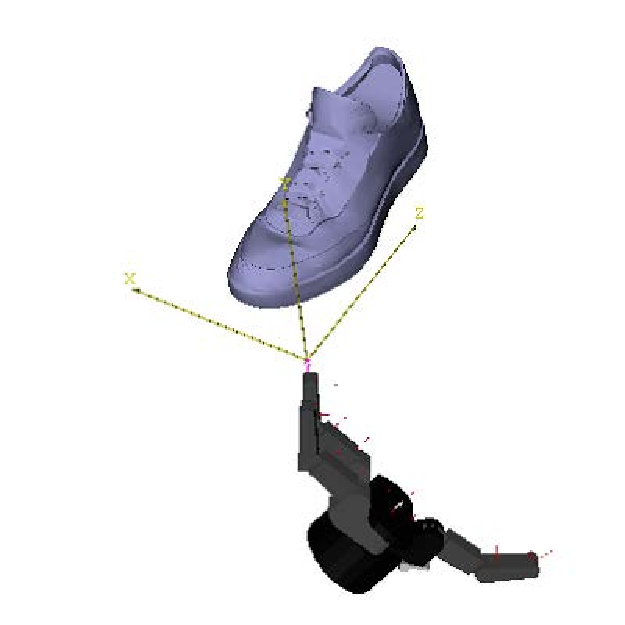
\includegraphics[width=4cm]{./fig_cha3/shoe_3i.pdf}}
    \vspace{0.3cm}
    \subfloat[\scriptsize{Final grasp 4}] {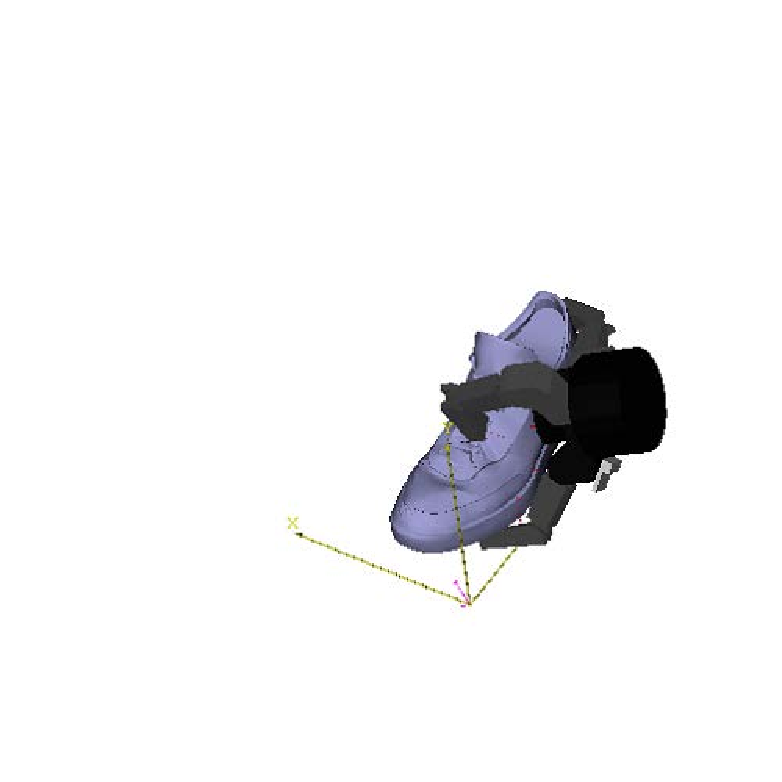
\includegraphics[width=4cm]{./fig_cha3/shoe_1f.pdf}}
    \subfloat[\scriptsize{Final grasp 5}] {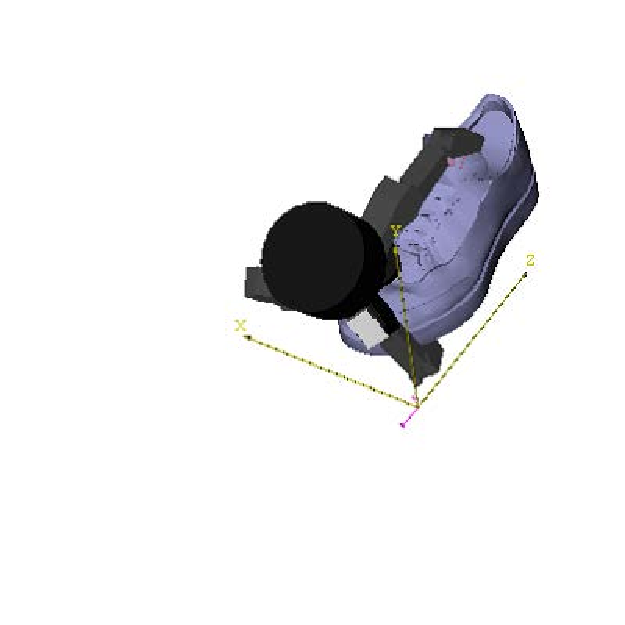
\includegraphics[width=4cm]{./fig_cha3/shoe_2f.pdf}}
    \subfloat[\scriptsize{Final grasp 6}]  {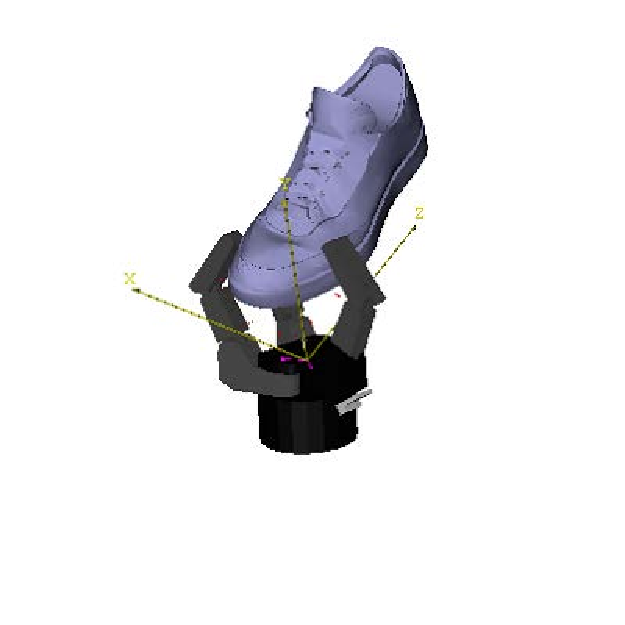
\includegraphics[width=4cm]{./fig_cha3/shoe_3f.pdf}}

  \caption{\scriptsize{Examples of Barrett hand grasping different objects (ashtray, shoe).
 The first and third rows (a,b,c and g,h,i) show the initial postures and the second and forth rows (d,e,f and j,k,l) show the corresponding final grasps.}
}
    \label{barrett}
\end{figure*}

\begin{figure*}
  \centering
    \subfloat[\scriptsize{Initial pose 7}]  {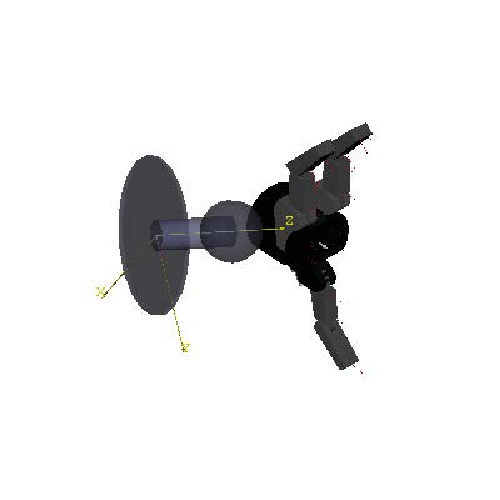
\includegraphics[width=4cm]{./fig_cha3/joy_2_i.pdf}}
    \subfloat[\scriptsize{Initial pose 8}] {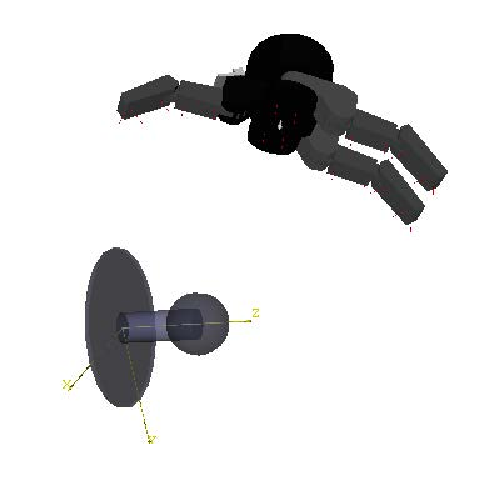
\includegraphics[width=4cm]{./fig_cha3/joy_3_i.pdf}}
    \subfloat[\scriptsize{Initial pose 9}] {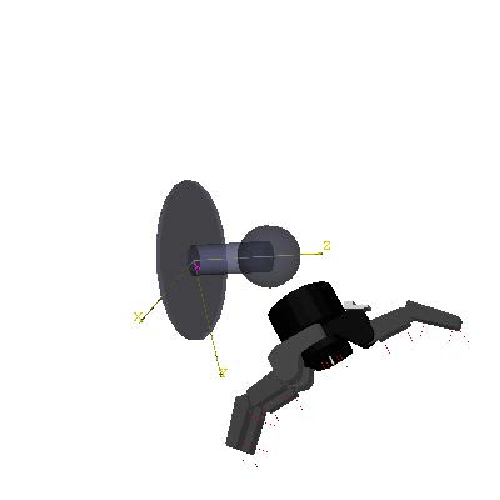
\includegraphics[width=4cm]{./fig_cha3/joy_5_i.pdf}}
    \vspace{0.3cm}
    \subfloat[\scriptsize{Final grasp 7}] {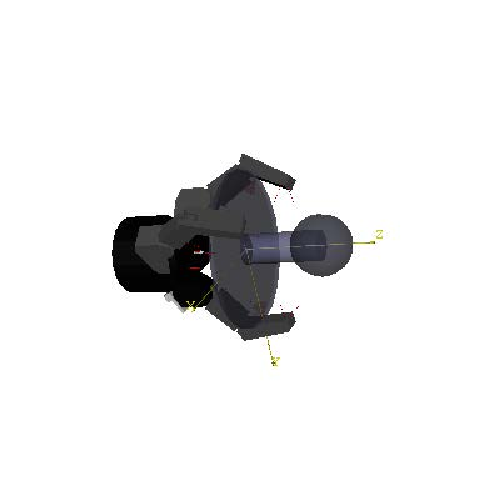
\includegraphics[width=4cm]{./fig_cha3/joy_2_f.pdf}}
    \subfloat[\scriptsize{Final grasp 8}]  {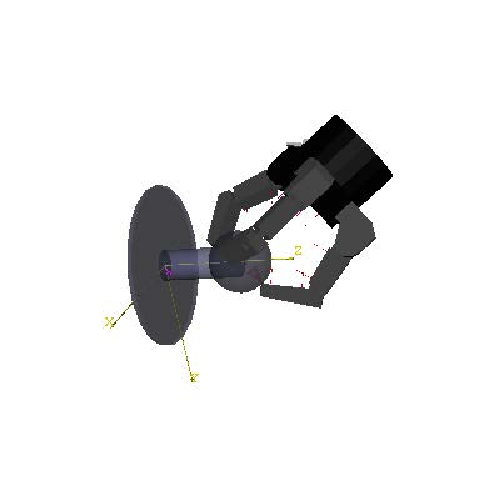
\includegraphics[width=4cm]{./fig_cha3/joy_3_f.pdf}}
    \subfloat[\scriptsize{Final grasp 9}]  {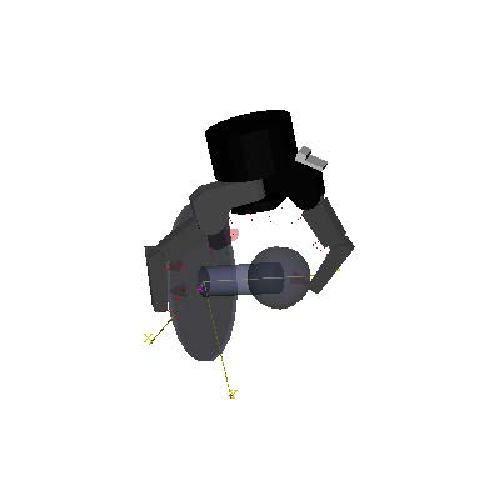
\includegraphics[width=4cm]{./fig_cha3/joy_5_f.pdf}}
    \vspace{0.3cm}
    \subfloat[\scriptsize{Initial pose 10}]  {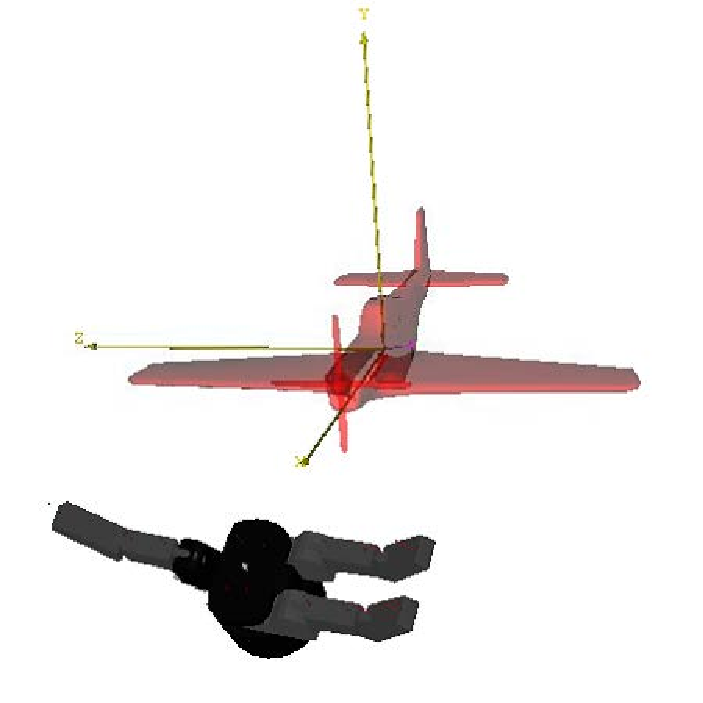
\includegraphics[width=4cm]{./fig_cha3/plane_2i.pdf}}
    \subfloat[\scriptsize{Initial pose 11}] {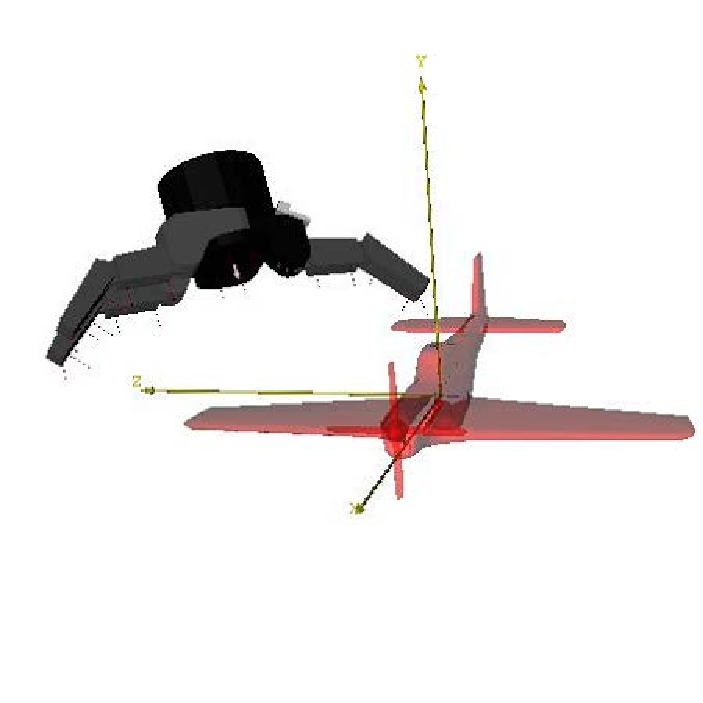
\includegraphics[width=4cm]{./fig_cha3/plane_3i.pdf}}
    \subfloat[\scriptsize{Initial pose 12}] {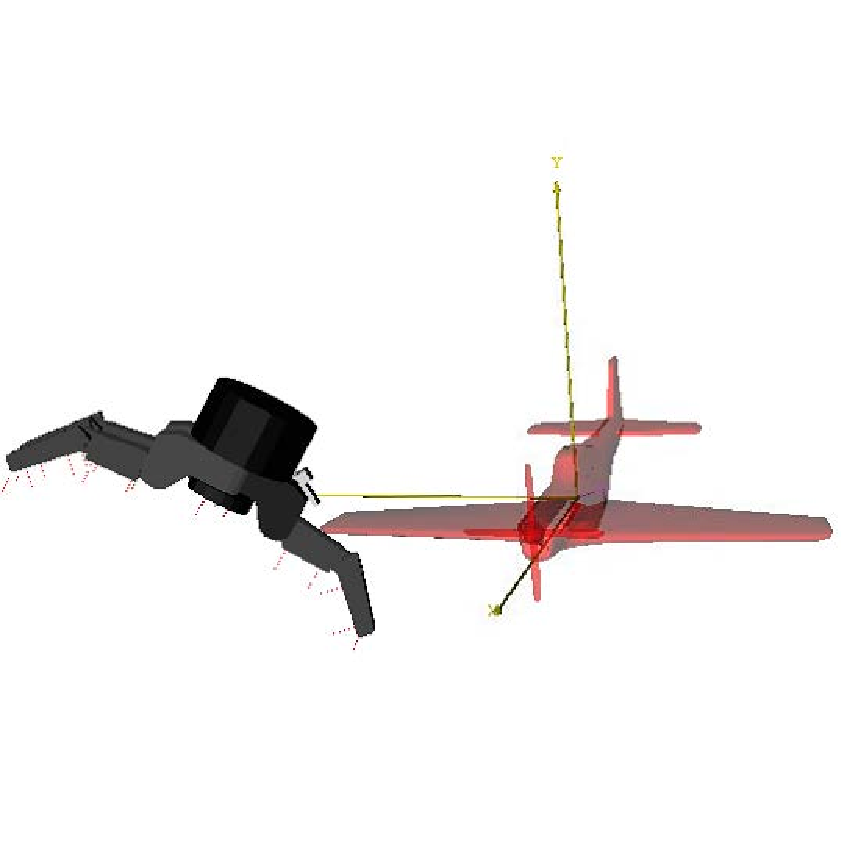
\includegraphics[width=4cm]{./fig_cha3/plane_1i.pdf}}
    \vspace{0.3cm}
    \subfloat[\scriptsize{Final grasp 10}] {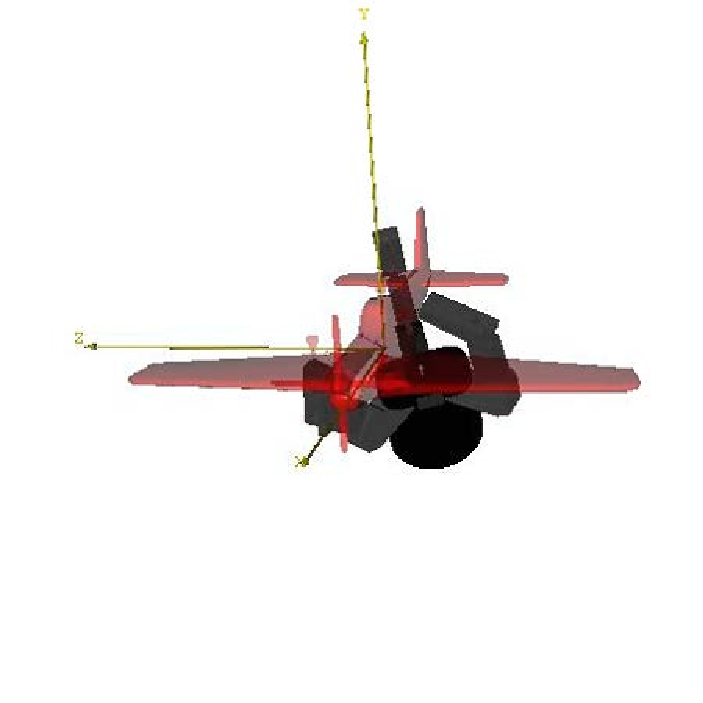
\includegraphics[width=4cm]{./fig_cha3/plane_2f.pdf}}
    \subfloat[\scriptsize{Final grasp 11}]  {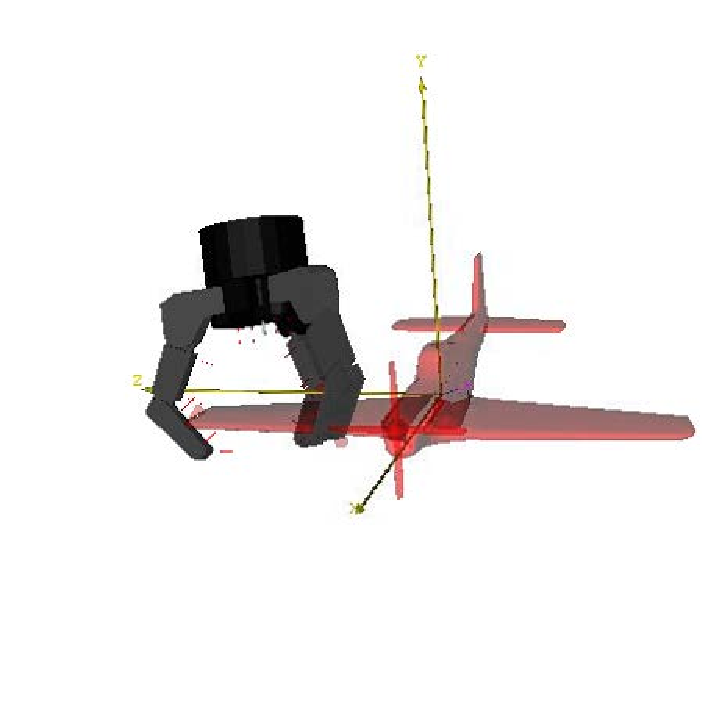
\includegraphics[width=4cm]{./fig_cha3/plane_3f.pdf}}
    \subfloat[\scriptsize{Final grasp 12}]  {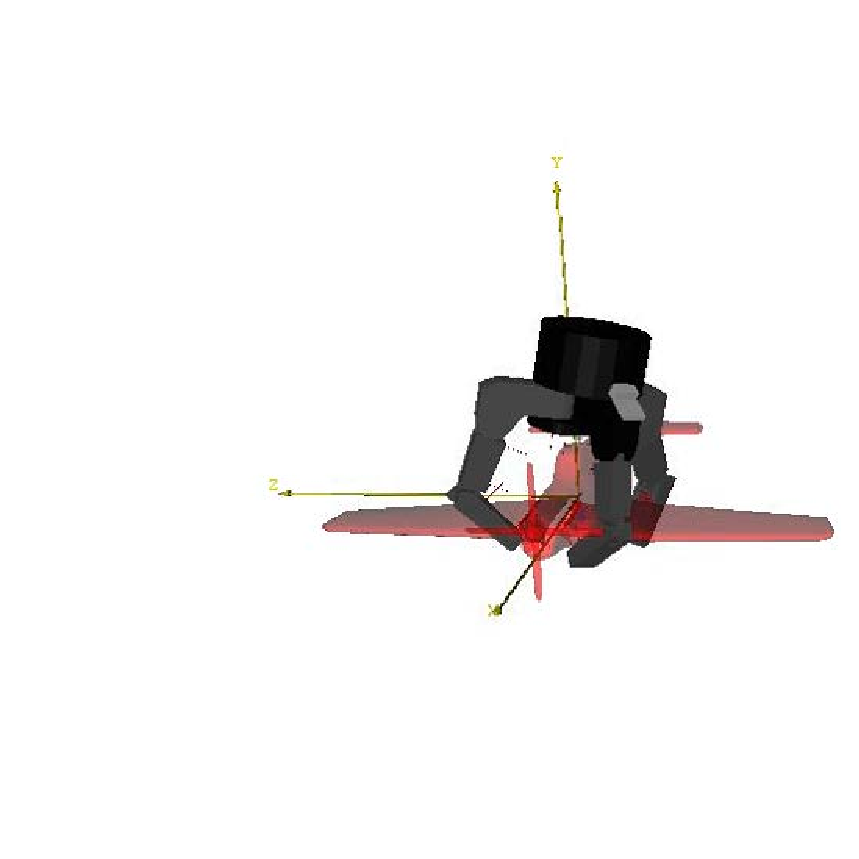
\includegraphics[width=4cm]{./fig_cha3/plane_1f.pdf}}

  \caption{\scriptsize{Examples of Barrett hand grasping different objects (joystick, aeroplane model). The first and third rows (a,b,c and g,h,i) show the initial postures and the second and forth rows (d,e,f and j,k,l) show the corresponding final grasps.}
}
    \label{barrett2}
\end{figure*}



%This approach provides a good estimation of a stable and feasible grasp for the given object and robot hand. In contrast to the common approach of learning from human demonstrations, these grasps are generated solely according to the mechanics of the robot hand. Some resulting grasps are markedly different from  human grasps, especially for the Barrett hand which is very different from the human hand. Our method may therefore out-perform human demonstrations in some contexts by better exploiting differences between human and robot ``physiology''.

To model the actual contact points between the robot hand and the object is difficult in real time because of the high dimensionality of the solution space and the non-linearity of the kinematic constraints. In our method, instead of computing the actual contact point position, we compute the most likely solution using a GMM. Though a certain amount of accuracy is traded off to achieve the real time goal, the overall performance is satisfying. In the experiments listed above, over 90 percent of the testing points find good grasps within a few milliseconds. This method is most efficient for objects with a smooth surface. For complex objects this method can achieve a high success rate of over 85\%. When grasping the parts requiring high precision, additional feedback from visual or tactile sensors is needed for further refinement of the grasp.

This approach requires the object model to be pre-trained. This is to say, we can only plan grasps for familiar objects with this method. It is useful for a robot working in a controlled environment with a limited number of objects, such as in operating theatres. For domestic service robots, however, this is not enough. New objects will continuously come to the house and hence the robot has to be able to grasp novel object shapes. An extension of this method to work on novel objects is discussed in the next two sections.

%The way we project the initial query point to the closest Gaussian component is more conservative.



\section{Grasping novel objects based on familiar parts}
\label{cha3:sec4}
A method to compute grasps for novel objects is in need for domestic service robots. In this chapter we study the problem of generating grasps for un-trained objects in real time.

Objects used in daily life have a variety of shapes. Very often they share similar shape parts, such as sphere, cylinder and box. These shapes repeatedly appear in our daily life, being the object shape or the part of the object shape. Hence we call them``shape primitives''.

To work with un-trained objects, we take the grasping by shape primitives approach~\citep{miller2003automatic}. This approach makes the assumption that all object shapes can be decomposed into a set of primitive shapes where grasps can be planned easily. Based on this assumption, we firstly build a set of GMMs to model the grasp distribution $\left(\Omega_i, i=1,2,...N\right)$ for a set of $N$ chosen shape primitives. When an unseen object is presented, of which the shape can be approximated as a combination of known shape primitives, it's grasp distribution is built by combining the primitives' models. The combined model is then used to quickly generate new grasps.

%\subsection{Combine grasp distribution of shape primitives}
%\label{cha3:sec4:combine}


\subsection{Primitive grasp distribution}
\label{cha3:sec4:pgdistribution}
%\subsubsection{Primitive grasp distribution}
%\label{cha3:sec4:combine:primitivegraspdistribution}
Here we define our shape primitives to be a set of superquadrics. We learn the grasp distributions for a set of superquadrics and use them as the ``primitive grasp distribution''.


\paragraph{Superquadrics} ~\\
%\label{cha3:sec4:combine:primitivegraspdistribution:sq}
Superquadrics are a family of geometric shapes that includes a large variety of shapes we use in daily life, such as cuboid, sphere and cylinder. We choose superquadrics as our shape primitives for three reasons. Firstly, superquadrics and their combinations can be used to represent most of the daily life objects. The wide use of superquadrics in computer graphics and the game industry for modelling object shapes shows its versatility. Secondly, all superquadrics are symmetric to their $x, y, z$ axis. This can reduce the number of testing grasps to 1/8. Thirdly, it's implicit expression is convenient for combining the grasp density, which will be explained in detail in the Section~\ref{cha3:sec4:combine:combining}.

To represent a superquadric we have:

\begin{equation}
r\left(x, y ,z\right) =
\left(\left(\frac{x-x_0}{a_1}\right)^{\frac{2}{\epsilon_2}} +
    \left(\frac{y-y_0}{a_2}\right)^{\frac{2}{\epsilon_2}}\right)^
    {\frac{\epsilon_2}{\epsilon_1}} +
    \left(\frac{z-z_0}{a_3}\right)^\frac{2}{\epsilon_1}
\end{equation}
where $\left(x_0, y_0, z_0\right)$ is the center, $a_1, a_2, a_3$ define the scale in the $x, y, z$ axis respectively, and $\epsilon_1, \epsilon_2$ define the shape of the superquadric.
We use the value of $r$ to measure the relative position of a point $x, y, z$ to the superquadric shape:
\begin{equation}
    r
    \begin{cases}
      <1, & \text{inside the superquadric}\  \\
      =1, & \text{on the surface of the superquadric}\ \\
      >1, & \text{outside the superquadric}
    \end{cases}
\end{equation}

For sphere, cylinder and box primitives, the shape parameters are:

\begin{enumerate}
\item Sphere: $\epsilon_1 = 1, \epsilon_2 = 1$
\item Cylinder: $\epsilon_1 = 1, \epsilon_2 = 0.1$
\item Box: $\epsilon_1 = 0.1, \epsilon_2 = 0.1$
\end{enumerate}

Figure~\ref{fig:sq}~ shows how does the shape varies by these two factors~\footnote{Figure from internet source http://www.vincent-morio.com/content/en/gallery.html}.

\begin{figure}
  \centering
  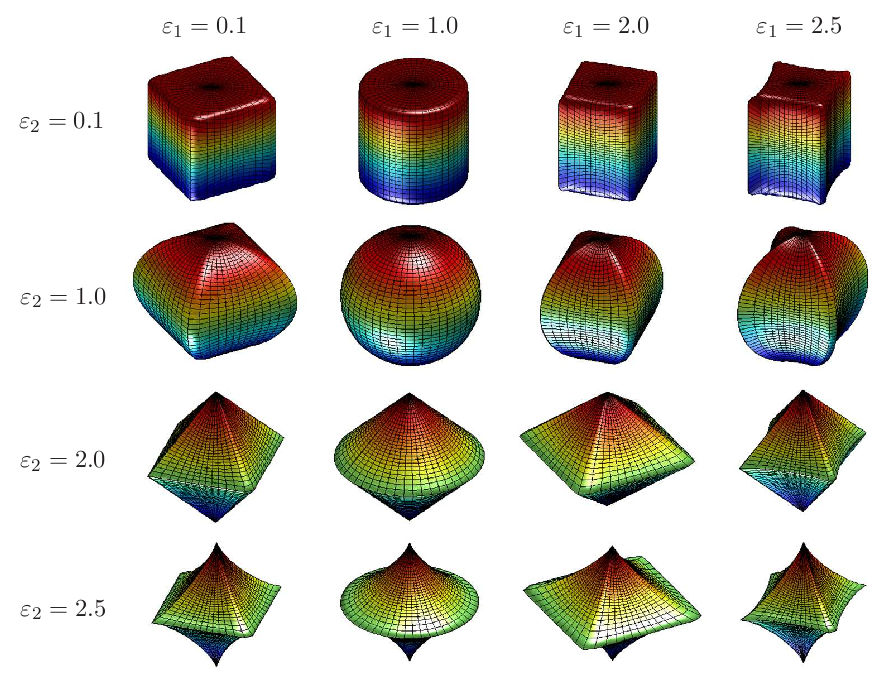
\includegraphics[width=14cm]{./fig_cha3/superquadrics.jpg}
  \caption{Illustration of 3D superquadric shapes with varying rounding parameters\protect\footnotemark.}
  \label{fig:sq}
\end{figure}


\paragraph{Learning grasp distributions for shape primitives}
%\label{cha3:sec4:combine:primitivegraspdistribution:learning}
~\\

With the method described in Section~\ref{cha3:sec2}, we build GMMs for the feasible grasp distributions for a set of shape primitives, i.e. superquadrics. Again, we model the distribution with a GMM as a sum of $K$ Gaussian components:

\begin{equation}
{
P (\boldsymbol{h},\boldsymbol{o},\boldsymbol\theta \text{\textbar} \varOmega)
= \sum_{k=1}^K {p_{k}p(\boldsymbol{h},\boldsymbol{o},\boldsymbol{\theta} \text{\textbar} {\boldsymbol{\mu}_k}, {\boldsymbol{\Sigma}_k})}
}
\end{equation}
where $k$ is the number of Gaussian components, $p_k$ the prior of the Gaussian component and the $\boldsymbol{\mu}_k$, $\boldsymbol{\Sigma}_k$ the corresponding mean and covariance.

Figure~\ref{fig:primtivedistr} visualizes the grasp distributions encoded by GMMs for three shape primitives: a box, a sphere and a cylinder. The robot hand we use here is the Barrett hand.

\begin{figure}
  \centering
    \subfloat[\scriptsize{Box}] {\includegraphics[width=4.5cm]{./fig_cha3/box1.eps}}
    \subfloat[\scriptsize{Sphere}]  {\includegraphics[width=4.5cm]{./fig_cha3/ball2.jpg}}
    \subfloat[\scriptsize{Cylinder}]  {\includegraphics[width=4.5cm]{./fig_cha3/cyl.jpg}}
  \caption{A 3D visualization of the feasible grasp distribution for three shape primitives and the Barrett hand. The red contours are the isosurfaces of the grasp distribution. The ``redder'' the area is, the denser the distribution is.}
  \label{fig:primtivedistr}
\end{figure}


\subsubsection{Combining grasp distribution} ~\\
\label{cha3:sec4:combine:combining}
For an object composed of a few shape primitives, its grasp distribution is the combination of the the grasp distributions of its primitive components. However, this ``combination'' is not a summation of the GMMs: we need to exclude the grasps causing collision.

Before combining the grasp distributions, which are encoded by GMMs, of different shape primitive components of an object, we need to reshape each GMM by the object geometry. This is because when primitives combine to a more complex shape object, the grasp space of one part might be blocked by other part of the object.

For example, an object combined by a cylinder and a sphere is shown in Fig.~\ref{fig:object}(a) and it's primitives with their grasp distributions are shown in (b) and (c). As can be seen in (b) and (c), the top part of the grasp distribution of the cylinder will be inside the sphere and the bottom part of the grasp distribution of the sphere will be inside the cylinder. Grasps generated from these parts will cause collisions between the hand and the object and hence they have to be excluded from the model. 
% Finger collision
%Further, even when the robot hand is placed in a feasible location for all components, when the fingers clutch to grasp one component of the object, the moving trajectory of the finger might be blocked by other components. These kind of grasps should also be excluded from the grasp density of the whole object.
%Therefore, we take into account two kinds of collisions: collisions between the palm and the object and collisions between the finger trajectories and the object. 
To avoid collisions, we use the ``object sigmoid'' function to remove the collision parts.

\paragraph{Object sigmoid} ~\\
\label{cha3:sec4:combine:sigmoid}
We define a shape descriptor ``object sigmoid'' for objects modelled by a superquadric. The object sigmoid is a 3 dimensional sigmoid function defined as:
\begin{equation}
s\left(x, y ,z\right) = \frac{1}{1+e^{-100\left(r\left(x, y ,z\right)-1\right)}}
\label{equ:objectsigmoid}
\end{equation}
where r$\left(x, y ,z\right)$ is a function of the location defined in the form of a superquadrics. When we model an object shape with a superquadric, the object sigmoid has different values inside, on and outside the object:
\begin{equation}
    s
    \begin{cases}
        \rightarrow0, & \text{inside the object}\  \\
        =0.5 & \text{on the surface of the object}\ \\
        \rightarrow1 & \text{outside the object}
    \end{cases}
\end{equation}
In equation~\ref{equ:objectsigmoid} we choose a large coefficient, i.e. 100, for $r$ to make a sharp transition between 0 and 1 and hence a sharp cut on the object surface. Hence the object sigmoid gives a description of the shape of the object in the space: zero inside the object and one outside the object.

Each primitive component has its own object sigmoid. Before combining the individual distributions to form the whole distribution, each individual distribution is multiplied by all other components' object sigmoids. In this way, the likelihood inside the other parts of the object is reduced to zero, while the likelihood outside the object remains. The grasp distribution is hence ``trimmed'' by the other components of the object. The grasp distribution of the whole object is the summation of all the trimmed grasp distributions:

\begin{equation}
\boldsymbol{\Omega}\left(x,y,z\right) = \sum_{i=1,2..}^{N}\left(\Omega_i\prod_{j=1,2..\left(j\neq{i}\right)}^{N}s_j\right)
\end{equation}
where $\Omega_i$, $s_j$, $N$ is the grasp distribution of the $i-th$ primitive component, the object sigmoid of the $j-th$ primitive component and the total number of primitive components. The total number of Gaussians in the GMM of the whole object is the sum of the number of each primitives.

Figure.~\ref{fig:object}(d) shows the resulting grasp distribution of the whole object, which is the combination of the trimmed grasp GMM of the cylinder (Figure.~\ref{fig:object}(d)) and the sphere (Figure.~\ref{fig:object}(f)). Strictly speaking, the combined grasp distribution is not a density function, as the integral of the probability of the whole space is not normalized to one. Despite this, it does not effect the computation of a new grasp as we consider each Gaussian component individually.

\begin{figure}
\centering
    \hspace{-1cm}
    \begin{minipage}[c]{1\textwidth}
    \subfloat[\scriptsize{Novel object}]  {\includegraphics[width=5cm]{./fig_cha3/object.jpg}}
    \subfloat[\scriptsize{Cylinder grasp distribution}] {\includegraphics[width=5cm]{./fig_cha3/cyl.jpg}}
    \subfloat[\scriptsize{Sphere grasp distribution}] {\includegraphics[width=5cm]{./fig_cha3/ball2.jpg}}



    \subfloat[\scriptsize{Combined object grasp distribution}] {\includegraphics[width=5cm]{./fig_cha3/cylball.jpg}}
    \subfloat[\scriptsize{Trimmed grasp distribution}] {\includegraphics[width=5cm]{./fig_cha3/cyl_sig.jpg}}
    \subfloat[\scriptsize{Trimmed grasp distribution}] {\includegraphics[width=5cm]{./fig_cha3/ball_sig2.jpg}}
    \end{minipage}

\caption{\scriptsize{(a) A combination of a cylinder and a sphere. (b) A 3D illustration of the grasp GMM of the cylinder. The red patch is the isosurface of the grasp GMM. (c) The grasp GMM of the sphere. (d) The combined grasp GMM of the whole object (d={e,f})). (e) The trimmed grasp GMM of the cylinder. The top part of the GMM is removed. (f) The trimmed grasp GMM of the sphere. Part of the bottom of the GMM is removed.}}
\label{fig:object}
\end{figure}


The equation above removes the grasps inside the object and hence avoids the collision between the robot palm and the object. 

% Finger collision
%However, grasps causing collision between finger trajectory and the object still remain.
%\paragraph{TODO: Trim grasp distribution by finger trajectory} ~\\


\subsection{Plan Grasp by combined grasp distribution}
\label{cha3:sec4:plan}

With the combined grasp distribution for the whole object, we can fast plan a grasp with the method described in Section~\ref{cha3:sec2}. Starting from an initial hand position and orientation $q = \{h, o\}$, the first step to compute a new grasp is to project $q$ to the feasible region of the GMM, where the probability of finding a stable grasp is high. This is done by finding the minimum Mahalanobis distance between $q$ and its projection point $q_k^\star$ in each Gaussian component of the GMM.

The projection point $q_k^{\star}$ of the $k$-th Gaussian component is computed as:
\begin{equation} \label{alpha}
q_k^{\star} = q + \alpha_k\left(q-\mu_k\right)
\end{equation}
where $\mu_k$ is the mean of the $k$-th Gaussian and $\alpha_k$ is a scalar determined by the boundary of the feasible region.

For $q_k^{\star}$ we have
\begin{equation} \label{qstar}
-\frac{1}{2}\left(q_k^{\star}-\mu_k\right)^T\Sigma_k^{-1}\left(q_k^\star-\mu_k\right)=-\frac{1}{2}\cdot{1}^{2}
\end{equation}
with equation~\ref{alpha} and~\ref{qstar}, $\alpha_k$ can be computed and hence $q_k^{\star}$.

The feasibility of each projection point is checked by the object sigmoids:

\begin{equation}
l_k = \prod_{j=1,2,...\left(j\neq{k}\right)}^N{s_j}
\end{equation}
If $l_k$ is smaller than 1, indicating that this point is inside or on the surface of the object, the likelihood at point $q^{\star}_k$ is zero.

We find the nearest projection point from the $q_k^\star$ with non-zero density. The nearest $q_k^\star$ is chosen to be the final grasp hand position and orientation $q^\star$. The grasp distribution $\Omega^{\star}$ which $q^{\star}$ locates in is used to compute the corresponding joint configuration though GMR. This allows us to compute the expected value of the finger joints from the conditional $p\left(\theta\mid{q^{\star}},\Omega^{\star}\right)$ (Section~\ref{cha3:sec2}). 
\section{Experiments of planning grasps for non-familiar objects}
\label{cha3:sec5}


\begin{table*}
\renewcommand{\arraystretch}{1.5}
\centering
\caption{Success rate and computation time of different methods and objects}
%\hspace{-2cm}
    \begin{tabular}
    { |>{\centering\arraybackslash}p{4cm}  | >{\centering\arraybackslash}p{2cm} | >{\centering\arraybackslash}p{3cm} |  >{\centering\arraybackslash}p{2cm} |  >{\centering\arraybackslash}p{2cm} |}
    \hline
    Approach and object & Force-Closure Grasp Found &  Mean of Computation Time($msec$) & Variance ($msec$)   \\ \hline
    Pre-trained grasp GMM for the novel object       & 98.1\%  & 13.8    & 0.015 \\ \hline
    Combined grasp GMM for novel object             & 92.1\%  & 21.9    & 0.011 \\ \hline
    Combined grasp GMM for spray flask              & 91.0\%  & 16.0    & 0.004 \\ \hline
    Combined grasp GMM for bedside table            & 82.2\%  & 21.1    & 0.006 \\ \hline
    \end{tabular}

\label{tab:result}
\end{table*}

\begin{table*}[ht!]
\renewcommand{\arraystretch}{1.5}
\centering
\caption{Shape primitives used in experiments}
%\hspace{-2cm}
    \begin{tabular}
    %{ | c | c | c |>{\centering\arraybackslash}p{3cm} |>{\centering\arraybackslash}p{3cm}|}
    {|>{\centering\arraybackslash}p{2cm}|>{\centering\arraybackslash}p{2.5cm}|>{\centering\arraybackslash}p{3cm}|>{\centering\arraybackslash}p{1.5cm} |>{\centering\arraybackslash}p{1.5cm}|}
    \hline
    Shape primitives& Object & Size($cm$) & Amount of training data & Number of Gaussians in GMM   \\ \hline
    Sphere 1        & Novel object (Fig.~\ref{fig:object})  & radius 7              & 12096    & 60 \\ \hline
    Cylinder 1      & Novel object (Fig.~\ref{fig:object})  & height 15 and radius 4& 15608    & 60 \\ \hline
    Box 1 & Spray flask (Fig.~\ref{fig:spr})        & $6\times9.5\times8$       & 9256    & 40 \\ \hline
    Box 2 & Spray flask (Fig.~\ref{fig:spr})        & $4\times11\times4.5$      & 7544    & 40 \\ \hline
    Box 3 & Spray flask (Fig.~\ref{fig:spr})        & $2.5\times4\times7$       & 3400    & 30 \\ \hline
    Box 4 & Bedside table (Fig.~\ref{fig:bedside})  & $52.5\times3\times52.5$   & 8668    & 20 \\ \hline
    Box 5 & Bedside table (Fig.~\ref{fig:bedside})  & $2.8\times57.6\times2.7$  & 4392    & 20 \\ \hline
    \end{tabular}

\label{tab:primitive}
\end{table*}

We test our approach initially on a novel object that is a combination of a sphere and a cylinder (Figure.~\ref{fig:object}(a) and Table~\ref{tab:primitive}). We choose to use the Barrett hand for the implementation as it is available in our lab. As explained above, the grasp of the Barrett hand is formulated as the combination of the hand position ($h$), orientation($o$) and finger joint angles($\theta$).  The grasp GMMs of the sphere and cylinder are pre-trained with randomly generated stable grasps from the simulator GraspIt!.

We compare this new approach with the previous approach that directly trained a grasp GMM for the whole object, by generating grasps for the object from 1000 starting points. Figure.~\ref{fig_result} shows a few resulting grasps. As shown in the Table~\ref{tab:result}, the success rate and the computation time of the new approach is of the same scale as the previous approach. The computation time is computed by Matlab on the same machine we use for the experiments described in Section~\ref{cha3:sec3} ( with a 2.8GHz processor and a 4GB RAM).


Further, we train 5 different boxes as our primitives (Table~\ref{tab:primitive}) and use them to approximate two daily life objects: a spray flask and a bedside table. The spray flask is approximated as the combination of box 1, 2 and 3 (Figure.~\ref{fig:spr}) and the bedside table is approximated as the combination of box 4 and 5 (three copies of box 4 as the surfaces and 4 copies of box 5 as the legs). The result is shown in Table~\ref{tab:result}. A few initial hand postures and their resulting grasps are shown in Figure~\ref{fig:spr_result} and~\ref{fig:result:bedside}.

%\vspace{-0.2in}
\begin{figure}[!ht]
%\vspace{-0.3cm}
\centering
    \subfloat[  {Initial pose 1}]  {\includegraphics[width=4.5cm]{./fig_cha3/8_i.jpg}}
    %\hspace{-0.01in}
    \subfloat[  {Initial pose 2}] {\includegraphics[width=4.5cm]{./fig_cha3/1_i.jpg}}
    %\hspace{0.01in}
    \subfloat[  {Initial pose 3}] {\includegraphics[width=4.5cm]{./fig_cha3/5_i.jpg}}
    %\vspace{0.05in}

    \subfloat[  {Final grasp 1}] {\includegraphics[width=4.5cm]{./fig_cha3/8_f.jpg}}
    \hspace{0.005in}
    \subfloat[  {Final grasp 2}] {\includegraphics[width=4.5cm]{./fig_cha3/1_f.jpg}}
    \hspace{0.005in}
    \subfloat[  {Final grasp 3}] {\includegraphics[width=4.5cm]{./fig_cha3/5_f.jpg}}

    \subfloat[  {3D projections}] {\includegraphics[width=7cm]{./fig_cha3/object_cylball_i_f_arrow.jpg}}
    \hspace{0.005in}
    \subfloat[  {2D contour projections}] {\includegraphics[width=6cm]{./fig_cha3/contour_Z_cylball_i_f_arrow2.jpg}}

\caption{  {Examples of Barrett hand grasping of a novel object. (a-d) Initial hand postures and final grasps. (g) A 3D illustration of the projection between the initial hand postures and the final grasps. (h) a 2D illustration of the interaction of GMM at $z$ = 0.}}

%\vspace{-0.2cm}
\label{fig_result}
\end{figure}

\begin{figure}
\centering
    \subfloat[  {}]  {\includegraphics[width=5cm]{./fig_cha3/spr.jpg}}
    \hspace{1cm}
    \subfloat[  {}] {\includegraphics[width=5cm]{./fig_cha3/box123.jpg}}
%    \hspace{0.01in}
\caption{  {(a) A spray flask. (b) A spray flask approximated by 3 boxes.}}
\label{fig:spr}
\end{figure}



\begin{figure}[!ht]
\centering
    \subfloat[  {Initial pose 1}]  {\includegraphics[height= 3cm]{./fig_cha3/spr_3_i.jpg}}
    \hspace{0.3cm}
    \subfloat[  {Initial pose 2}] {\includegraphics[height= 4cm]{./fig_cha3/spr_4_i.jpg}}
    \hspace{0.3cm}
    \subfloat[  {Initial pose 3}] {\includegraphics[height= 4cm]{./fig_cha3/spr_6_i.jpg}}

    %\vspace{0.05in}
    \subfloat[  {Final grasp 1}] {\includegraphics[width=4cm]{./fig_cha3/spr_3_f.jpg}}
    \hspace{1.5cm}
    \subfloat[  {Final grasp 2}] {\includegraphics[height=4cm]{./fig_cha3/spr_4_f.jpg}}
    \hspace{0.3cm}
    \subfloat[  {Final grasp 3}] {\includegraphics[width=4cm]{./fig_cha3/spr_6_f.jpg}}

\caption{  {Examples of Barrett hand grasping of a spray flask. }}
%\vspace{-0.8cm}
\label{fig:spr_result}
\end{figure}


\begin{figure}
\centering
    \subfloat[  {}]  {\includegraphics[width=5cm]{./fig_cha3/bedside.jpg}}
    \hspace{0.07in}
    \subfloat[  {}] {\includegraphics[width=5cm]{./fig_cha3/bedside_box.jpg}}
%    \hspace{0.01in}
\caption{  {(a) A bedside table. (b) A bedside table approximated by 7 boxes.}}
\label{fig:bedside}
\end{figure}

\begin{figure}
\centering
    \subfloat[  {Initial pose 1}]  {\includegraphics[width=4cm]{./fig_cha3/bed_6_i.jpg}}
    \hspace{0.2cm}
    \subfloat[  {Initial pose 2}] {\includegraphics[width=4cm]{./fig_cha3/bed_3_i.jpg}}
    \hspace{0.7cm}
    \subfloat[  {Initial pose 3}] {\includegraphics[width=4cm]{./fig_cha3/bed_5_i.jpg}}
    %\vspace{0.05in}

    \subfloat[  {Final grasp 1}] {\includegraphics[width=4cm]{./fig_cha3/bed_6_f.jpg}}
    \hspace{0.005in}
    \subfloat[  {Final grasp 2}] {\includegraphics[width=4cm]{./fig_cha3/bed_3_f.jpg}}
    \hspace{0.005in}
    \subfloat[  {Final grasp 3}] {\includegraphics[width=4cm]{./fig_cha3/bed_5_f.jpg}}


\caption{  {Examples of Barrett hand grasping of a complex shape bedside table (a-d) Initial hand postures and final grasps. }}
\label{fig:result:bedside}
\end{figure}


%$\bullet$ TODO: grasp density can be used to find grasps by task (Detry)
%$\bullet$ TODO: can not find grasps over different parts
%$\bullet$ TODO: interpolate primitives?
%$\bullet$ TODO: human spend more time on new object
%$\bullet$ TODO: take volume of robot hand into account
%In implementation we found the success rate depends on how well we can approximate the novel object with known shape primitives, and hence the choice of the shape primitives is important.Future work will focus on studying how to interpolate the grasp GMM for different shape primitives, to allow the novel objects to be approximated more precisely.


\section{Discussion}
\label{cha3:sec6:discussion}

We presented a method for computing grasps in real time. This is demonstrated on two very different robot platforms: the iCub hand and the Barrett hand. The result shows that the method can capture the versatility of grasps that are typical of grasps performed by an industrial gripper, and those that can be performed by a humanoid hand.
With the computation time in the millisecond scale,
this method would enable the robot to react quickly in robot-human interaction, such as picking up heavy objects from a person's hand, as well as adopting to fast perturbations in a dynamic environment.

We achieve this goal by using a closed-form solution. A GMM model is learned from the grasping demonstration generated offline for a given object. During the online execution no iterative method is used, we only need to solve a few equations with basic arithmetic operations. Hence the computation time is significantly shorter than the conventional optimization methods. Though we need to pre-train the robot to grasp different objects, in many scenarios such as surgery assistance, robots and humans must work with a predefined set of objects. This allows us to build the grasping model for each object beforehand.


To find the closest Gaussian component we used the Mahalanobis distance rather than the Euclidean distance. The advantage of this is that it takes into account the correlations among each dimension of the hand configuration. In a space of different types of measurements, i.e. length and angle, Mahalanobis space is a better representation than the Euclidean space. Indeed, humans do not always use the Euclidean distance to select their grasps. We may move our hand further than needed to grasp an object, in order to avoid flipping our hand to another orientation.

Our approach provides a good estimation of a stable and feasible grasp for the given object and robot hand. To model the actual contact points between the robot hand and the object is difficult in real time because of the high dimension of the solution space and the non-linearity of the kinematic constraints. In our method, instead of computing the actual contact point position, we compute the most likely solution using a GMM. Though a certain amount of accuracy is traded off to achieve the real time goal, the overall performance is satisfying. In our experiments, over 90 percent of the testing points find good grasps within a few milliseconds. This method is most efficient for objects with a smooth surface. For complex objects this method can achieve a high success rate of over 85\%. When grasping the parts requiring high precision, additional feedback from visual or tactile sensors is needed for further refinement of the grasp.

When extending this approach to grasp non-familiar objects, we exploit an modular approach: grasp by shape primitives. The grasp distribution is learnt for each shape primitive and is combined to form the distribution for the whole object. Experiments show that this method enable the robot to grasp complex objects with high successful rate (over 80\%) while maintaining the computation time with in millisecond scale. 

%The way we project the initial query point to the closest Gaussian component is more conservative.
In contrast to the common approach of learning from human demonstrations,
these grasps are generated solely according to the mechanics of the robot hand.
Some resulting grasps are markedly different from  human grasps, especially for the Barrett hand which is very different from the human hand.
Our method may therefore out perform human demonstrations in some
contexts by better exploiting differences between human and robot ``physiology''. 





\chapter{Learning human manipulation skill}
\label{cha4}
% Motivation - Methodology - Experiment - Result - Discussion

\section{Introduction}
\label{cha4:sec1}
% Motivation
% OM is important: what it can do? how it helps human?
In our daily life, object manipulation is one of the most commonly used skills. It includes a large category of activities ranging from the simple pick-and-place task to the complicated dexterous manipulation task, like writing or using chopsticks. Service robots won't be able to really ``serve'' humans without these manipulation abilities. Enabling robots to carry out manipulation tasks can alleviate human workload and free humans from many chores. However, robots with human level manipulation skills still only exist in science fiction.

% OM is difficult: why it is difficult?
Generally, manipulation tasks are very difficult for robots. Distinct from pure motion planning, manipulation planning aims to not only move the robot to a desire state, but also to change the environment to a desired state. Therefore in addition to robot motion planning, the impact of the robot on the environment, i.e. robot environment interaction, has to be planned. The object interactions are usually complex and hard to predict as they involve complicated contact situations, and the changing kinematics and dynamic properties of the environment. The complicated physics in object interactions make manipulation tasks difficult. The multi-body interactions and the effects of friction can cause abrupt changes in the environment. This makes the environment non-linear and non-stationary.

% What is solution to OM? - adaptive control. What is AC? Benefit of AC, but difficult to design.
Control methods depending on invariable 
\textcolor{red}{invariant, or unvarying but not invariable (you choose!)}
environmental parameters are not efficient for most manipulation tasks. Adaptive control methods, which focus on handling varying parameters and initial uncertainly, are required for manipulation. An adaptive control strategy is usually hard to design, especially when it involves a complex environment. This demands deep inside \textcolor{red}{knowledge of} the task and the kinematic and dynamic properties of the environment.

% learn AC from human demonstration: benefit...
To this end, we conduct a learning from human demonstration approach to gain an adaptive control strategy. This approach has two-fold benefits: Firstly, we do not need to analytically derive the the kinematic and dynamic properties of the environment in order to design the controller. Secondly, it provides a framework to easily program a robot with a task skill. With an increasing use of robots in daily life, more and more tasks will need to be programmed. Non-linear control methods are usually limited to narrow categories of tasks and hence need to be carried out task by task. It is impractical to pre-program all such object manipulation tasks manually. Learning from human demonstration enables even non-programmers to program robots to do various kinds of tasks quickly.

% what human do: prediction
Humans can perform these skilled tasks and adapt to the changes without difficulty. At the heart of this skill is prediction~\cite{flanagan2006control}. Studies from neuroscience suggest that humans develop internal models for motor control, to predict the future state of the environment. By comparing the predictive state with the actual sensory state, the internal models monitor the progression of the tasks and launch the corresponding motor corrections and motor reactions to adapt.

%To handle these situations, robots have to be equipped with a nonlinear and non-stationary control strategy, which is hard to design by analytical approaches.

% Conventional AC is difficult, use modular. benefit of modular
Inspired by this concept, we propose an approach to learn a human adaptive control strategy. This adaptive control strategy is encoded with a modular model, which allows fast adaption to non-linear and non-stationary systems. Each module includes a forward model for context estimation and an inverse model for motor command generation. From multiple human demonstrations, we extract a set of strategies, each of which is responsible for one specific task context. Using this method, we modularize the human adaptive control strategy. Internal models (a forward model and an inverse model) are learnt within each module with a representation that can be easily transferred to a robot. When a robot executes a similar task, the forward models estimate the context of the task and \textcolor{red}{once} ``contextized'' \textcolor{red}{'contextualised' would be better throughout I think} the inverse models \textcolor{red}{are able to} generate proper commands to drive the \textcolor{red}{robot}.
Each learned control strategy is weighted by the similarity of the current task context and its corresponding context. The optimal strategy is computed as the linear combination of the weighted commands of each strategy.

This approach does not require any prior knowledge of the kinematics nor dynamics of the system, nor is it restricted to a specific robot platform. The control strategy is learnt at the object level and hence can be transferred from human to robot directly.
This work contributes a framework to modularize human adaptive control strategies for manipulation tasks and to transfer the learned internal models to a robot. To verify our approach, we use a \emph{Opening Bottle Caps} task as an experiment. An adaptive control strategy is required here, as the friction between the bottle and the cap surfaces has multiple phases. We modularize the human control strategy in this task and implement it on a robot to open both familiar and novel bottles.

In the next few sections, I will present our approach of learning a multiple module model of a human manipulation strategy~\ref{cha4:sec1}, detail the experimental setups~\ref{cha4:sec2} and discuss the results~\ref{cha4:sec3}.

\section{Modular approach in manipulation}
\label{cha4:sec2}


This section presents the method we used to modularize human demonstration of manipulation tasks. Our goal was to acquire a modular based control policy for an object manipulation task from human demonstration. To this end, we take a three step approach:
\begin{enumerate}
\item Human demonstrating a task in different contexts (Section~\ref{cha4:sec2:demo}).
\item Extracting human control strategies for different contexts and building multiple internal models(Section~\ref{cha4:sec2:learn}).
\item Use the multiple models to compute motor commands for a robot(Section~\ref{cha4:sec2:control}).
\end{enumerate}

Figure~\ref{fig:overview} shows an overview of our framework.

\begin{figure}
  \centering
   \includegraphics[width=15cm]{./fig_cha4/overview3.pdf}
  \caption{ \scriptsize{System overview.}
  \label{fig:overview}
}
\label{fig:demo}
\end{figure}

\subsection{Human demonstrating tasks involving direct contact with objects}
\label{cha4:sec2:demo}


\begin{figure*}
  \centering
    \subfloat[\scriptsize{Optitrack markers attaching to a cap}] {\includegraphics[height=4cm]{./fig_cha4/marker2.jpg}}
    \subfloat[\scriptsize{Force torque sensor}] {\includegraphics[height=4cm]{./fig_cha4/Nano25-E.jpg}}
    \subfloat[\scriptsize{Texscan tactile sensors mounting to a glove}] {\includegraphics[height=4cm]{./fig_cha4/texscan2.jpg}}
    \caption{\scriptsize{Sensors used in the human demonstration of opening a bottle cap task.}}
  \label{fig:devices}
\end{figure*}

%Learning manipulation tasks is one of the main application of this approach. The physical properties of a manipulation task is hard to express analytically, and as a result the control strategy is hard to derive. Modeling expert's demonstration of strategies has been used as an alternative to the analytical solution.

The first step is to demonstrate a task to a robot. Two major forms of demonstration are used in teaching manipulation tasks: kinematics teaching and tele-operation.

\paragraph{Kinematics teaching} ~\\
% ===== Why not kinematics approach? =====
In kinesthetic teaching, humans directly make contact with the robot and guide their movements to accomplish a task~\cite{korkinof2013online,pais2014encoding,pastor2011skill,Miao2014}. The trajectory of movements and contact force are recorded by the robot sensors.
This method is simple and effective but limited in the number of controllable end effectors. While a manipulation task usually involves multi-finger movement, a human can kinematically operate one finger with each hand and hence two fingers simultaneously at most. Hence kinesthetic teaching is not feasible for demonstrating multi-finger tasks.

\paragraph{Tele-operation teaching} ~\\
To control multi-finger hands, some researchers use tele-operation~\cite{bernardino2013precision,kondo2008recognition,Fischer98}. This usually relies on data gloves to sense hand posture, and a motion capture system to sense human hand-arm motions. The human motion is mapped to robots to generate motions and interact with the environment. In fine manipulation tasks, the robot platforms are usually restricted to anthropomorphic hands for better mapping. All of the above methods provide no direct force feedback to the human demonstrator during manipulation.

\paragraph{Human direct demonstration} ~\\
In some studies, the human demonstrates manipulation tasks with their own body~\cite{asfour2008imitation}. With direct interaction with the object, a human is able to perform the task most naturally and with a more delicate control strategy. The task information captured from these human demonstrations needs to be transferred to robots. Because the difference of the embodiment between human and robot, a mapping between them has to been built. Various mapping methods have been proposed~\cite{do2011towards,asfour2008imitation,hueser2006learning}, while human correction~\cite{calinon2007incremental,sauser2011iterative,romano2011human} and self-correction via learning~\cite{bidan2013robio} are proposed as alternative solutions. These methods are quite robot specific and task specific. In general, how to effectively transfer human skill to robots skill remains an open problem.

Here we use a method to allows the subject to perform natural feedback control strategies in demonstration, while the strategy can then be easily transferred to any robot platform. In our task demonstrations, a human wears tactile sensors and directly interacts with objects. In this way, human demonstrators have direct cutaneous and kinaesthetic feedback, which is desirable for good manipulation demonstration. To make the information embedded in the demonstration easily transferable to robots, the demonstration is expressed from an ``object centric viewpoint''.


%============= Object Centric =============
\paragraph{Object centric representation} ~\\
The object centric viewpoint considers a manipulation task from the object's perspective, which suggests the goal of learning a manipulation task is to reproduce the same object behaviour, rather than reproduce the demonstrator's movement. This makes sense as humans may use different methods to accomplish a manipulation task: the motion or posture might be different but the effect on the object is the same. What the robot needs to imitate is the effect on the object but not the movements.
Hence our approach takes this principle and learns a control strategy to produce a desired object behaviour, rather than to produce a human or robot behaviour. This strategy expressed from the object perspective can be transferred to a robot platform by converting the exerted force to the robot's joints' torque with a Jacobian matrix. From the object centric viewpoint the manipulation problem is simplified: we transfer from a problem of controlling multi-finger (multi-end-effector) and its impact of the environment to controlling an object.

Based on this object centric principle, we record the object trajectory and \textcolor{red}{the forces driving it}. This data can be accessed by a motion capture system, force-torque sensors and a wearable haptic device. Fig.~\ref{fig:devices} shows a few sensors we used in the opening bottle caps task. The representation of the data will be explained in Section~\ref{cha4:sec2:learn:objectlevel}


% ======= demonstrate in different context   =======
\paragraph{Demonstrations in different task contexts}  ~\\
During the demonstrations, the teacher performed a task a number of times to generate enough data to capture the key features. Further, the teacher performed the task under different system kinematics and dynamics configurations, e.g. friction conditions, in order to explore how humans adapt to different task contexts. These different configurations are chosen to cover a wide range of different contexts. These wide ranging demonstrations are then used to learn a multiple module model.





\subsection{Learning a Multiple-Module Model}
\label{cha4:sec2:learn}
In this section we detail our modelling method, explaining why we use modular approach and how we model human manipulation strategies.

%% Internal model
%In the study of human motor control, internal model is one of the most evidently supported hypothesis. It postulates a neuron process that simulates output of the motor system and the environment~\cite{kawato1999internal}. It's applications in robot control have been explored by many researchers. Various types of internal models are built for different tasks~\cite{sciavicco2000modelling,jordan1992forward}.

% Adaptive
A modular approach is used in adaptive control and its benefit has been long discussed~\cite{jacobs1991adaptive,narendra1997adaptive}.
In manipulation tasks, context changing is a common phenomenon due to object interactions. These changes are often rapid or discontinuous. Classic adaptive control approaches such as model identification~\cite{khalil2004modeling} are inadequate for these tasks, as instability or error may occur during the optimization of the model variables. To adapt quickly, the multiple model approach~\cite{narendra1995adaptation}, referred to as the modular approach here, is proposed. In this approach, multiple controllers are designed, each of which is in charge of a certain task context. During control, the task context is estimated online and the corresponding controllers are activated.  Some recent work~\cite{fekri2007robust,kuipers2010multiple,sugimoto2012emosaic} presents promising modular based approaches.

% Modular - human MOSAIC

%%The excellent ability of human to manipulate different objects in different contexts and to quickly adapt to change of contexts suggested that our central nervous system (CNS) maintains multiple internal models            of outside environments, rather than a single internal model that adapts to new environment~\cite{neilson1985acquisition}.
%Based on the concept of modularity, the Modular selection and identification for control (MOSAIC) architecture was proposed to explain the motor control strategy of the CNS~\cite{wolpert1998multiple}. According to this hypothesis, during the motor control process, the brain quickly select the most appropriate modules according to the current environment context and use them to generate an appropriate motor command to react to the environment~\cite{haruno2001mosaic}.

% Our approach
The excellent ability of humans to manipulate different objects in different contexts and to quickly adapt to changes of context suggest that our central nervous system (CNS) maintains multiple internal models of outside environments, rather than a single internal model that adapts to new environment~\cite{neilson1985acquisition}. Indeed, neuroscience evidence suggests that animal brain sum modular stimulates of muscles to generate different motions~\cite{mussa1994linear}
\textcolor{red}{re-write this sentence as it is bad english and I'm not sure exactly what you are trying to say}.
Inspired by this, we take a modular approach to model the human adaptive control strategy.



%\paragraph{Our modular strategy} ~\\
The modular approach we take is inspired from MOSAIC (Modular selection and identification for control)~\cite{haruno2001mosaic}, one of the pervasive multiple module models for human motor control mechanisms.

The system of MOSAIC is constituted by multiple parallel modules. Each module has three components: a forward model, an inverse model and a responsibility factor (RF). The forward model is responsible for estimating the task context in real time, and the inverse model is used to generate appropriate motor commands for the context. These two models are connected by the RF. The task context estimated by the forward model is compared with the actual current task context.
The RF of each module is computed according to the accuracy of the estimation: the more accurate the forward model predicts, the higher the RF is (detailed in Section~\ref{cha4:sec2:control:rf}). The RF's of all modules are computed and then normalized.
The inverse models are weighed by their normalized RF. The final motor command is the linear combination of the commands factored by their weighs. With this mechanism, the modules best predicting the current task context take more responsibility in the final motor command. Figure~\ref{fig:control} sketches the work flow of this system. Though MOSAIC has gained a large concerns \textcolor{red}{do you mean a strong reputation?} in the neuroscience community, this approach is not widely used in robot control.

We take this paradigm, and model our internal models using GMM. Training GMM with the Expectation Maximization algorithm (EM), we estimate the optimal values of the model parameters. Compared to the early work~\cite{wolpert1998multiple} which use Neural Networks and have to manually tune the variance of each forward model, GMM has the advantage of automatically computing the all the model parameters. Later work~\cite{haruno2001mosaic} fixes the hand tuning problem by modelling with a Hidden Markov Model (HMM) and optimizing the model with EM. With this method the forward models are assumed to be linear. In our approach, GMM allows a non-linear system to be modelled. Fig.~\ref{fig:control} illustrates the workflow of our approach. Compared to the switching modular method~\cite{narendra1997adaptive}, i.e. only one module will be activated and used to generate motor command, the linear combination of the modules requires a smaller number of modules to approximate the system dynamics.

In some tasks the forward model and inverse model are united into a single model~\cite{petkos2006learning}. For that particular task the action ($a_t$) taking the current task state ($s_t$) to the desired task state ($s_{t+1}$) is always unique. However, in many cases this mapping is not unique and hence the inverse model has to include extra variables in order to resolve the non-uniqueness. In our approach we build the forward and inverse models separately.
%However this model does not provide a method to find out number of models needed in tasks. %and the inverse model represented by the joint distribution will potentially produce an invalid command that average all possible solutions.

Despite the many applications and discussions of the modular approach, how to systematically modularize the control strategy presented during the human demonstration, i.e. how to determine the number of modules and build an appropriate model for each module, still remains an open problem. We tackle this problem with a data driven approach. We cluster the demonstration data with a hierarchical approach and model each cluster as a pair of forward and inverse models. This solution can be applied to modularize many manipulation tasks. A similar clustering method has been applied to group and build tree structures of human motion pattern primitives~\cite{kulic2008incremental}. To cluster the motion primitives, a high value and a low value of the cut off parameter are tested to evaluate the trade off effect between facilitating quick tree formation and introducing misclassification. In our approach, the cut off parameter is determined by the variance of the data and hence avoids this step. This provide us with a proper grouping of the data which can then generate proper motor commands for control. To the best of our knowledge, our work is the first realization of the modular approach in learning an object manipulation task with a real robot.

%
%
%Scientist has long been fascinated by human adaptive motor control ability and wondering the mechanism of it. One of the most evidently supported hypothesis is the multiple model~\cite{neilson1985acquisition}. %~\cite{haruno2001mosaic}



\subsubsection{Object centric manipulation strategy}
\label{cha4:sec2:learn:objectlevel}


As mentioned in Section~\ref{cha4:sec2:demo}, one of the challenges in imitation learning is the mapping problem, i.e. how to map the teacher's motions to the robot's motions so that they produce the same effects. This mapping becomes more difficult for object manipulation tasks, the goal of which is to deliver the object from the current state to a desired state. During this process the movement of the manipulator is bounded not only by its own kinematic constraints but also bounded by by the movement of the object. It is more important to imitate how humans apply forces to achieve an object's desired movement, than to imitate the human limb movement.
Therefore we take an ``object centric approach"~\cite{okamura2000overview}, where the control policy is taken from the object's perspective.


Therefore, our model encodes a force and torque profile rather than the end-effector movement trajectory. The imitation learning objective here is not to find a policy for the end-effector movement but to find a policy that maps the force and torque to the object movement. This policy allows the robot to efficiently acquire new behaviours to accomplish the task. %Different robots move differently to achieve the desired object movements.
Given the robot's kinematics and the desired force to be exerted on the object, the joint torques can be deduced by the Jacobian matrix~\cite{okamura2000overview}. To this end, we focus on the force-torque-displacement tuple: $\{F,\tau,s\}$ demonstrated in the task. In later sections, we refer $\{F,\tau\}$ as the motor command with notation $\{a\}$. In each demonstration, a time series of the tuples is recorded.



\subsubsection{Decide number of modules}
\label{cha4:sec2:learn:cluster}

% ----------- why clustering -----------
Due to object interaction, manipulation tasks frequently encounter abrupt changes in system dynamics, e.g. transfer between statuses \textcolor{red}{do you mean 'states' in this sentence?} with no contact and with contact, between statuses driven by static friction and by driven dynamic friction. Different strategies should be used to handle different dynamics and hence a multiple module model is desired. Our approach is to extract different strategies from demonstration and build one module for each of the strategies. During implementation, the system can quickly estimate the context by the sensory inputs and weight the modules according to their reliability and then generate a contextualized motor command.

% ---------- Cluster to find number of modules -----------
Different tasks may need a different number of modules. This number may not be easy to find. In previous studies~\cite{sugimoto2012emosaic,haruno2001mosaic}, the number of modules is defined as the number of different target objects or different phases in the task, which can be clearly distinct, such as no load or on load. However this is not always the case. In a task involving more phases, humans may regard different phases as the same task context and handle them with the same control strategies. A recent study suggests that modularizing a control strategy by the number of objects can cause redundancy of modules and hence is inefficient~\cite{lallee2009}.

Here we propose a data-driven approach to properly define the number of modules for a given task.
To this end, we should differentiate different types of strategies. The differences can be reflected from the different patterns of the force-torque-displacement tuple. We differentiate the patterns by clustering. Data in the same cluster is considered to be governed by the same strategy. The number of clusters is the number of modules and each module is encoded by one model.


% ----------- Distance Metric for clustering ------------
The goal of clustering is to separate a set of data into a few groups according to their similarities, such that the data in the same group are more similar to each other than those in different groups. This technique has very important applications in computer vision and language processing~\cite{warren2005clustering}. Numerous clustering algorithms have been proposed for different purposes.

Before clustering, we need to measure the similarities, i.e. the distances, between the data points we want to cluster. The similarity metric is user defined according to the purpose of clustering. One of the mostly used metrics is the Euclidean distance. Different from the usual clustering problem, however, the data we need to cluster are not a set of single data points but a set of time series. Each time series includes a sequence of data points. Here we use the Dynamic Time Warping technique (DTW) to measure the distance between each pair of time series~\cite{berndt1994using}.

\paragraph{Dynamic time warping} ~\\
%%%%%%%%%% TODO: DTW explaination, citation.
Dynamic time warping is a technique for measuring the similarity between two time series, which may have different speeds or durations. It has an important application in speech recognition. For example, two people may utter the word ``hello'' at different speeds. Using DTW, one is able to tell that they are speaking the same word. This is achieved by warping the single \textcolor{red}{series?} in the time dimension. The two time series' are ``aligned'' by finding their optimal match. The similarity is computed as the average distance between the corresponding points of the two time series. By this method, the similarity computed by DTW is independent of the variance in the time dimension. Figure~\ref{fig:alignDTW} shows an example of the alignment of two time series by DTW.

Here we make an assumption that our manipulation task is time independent, i.e. in the time scale, whenever we apply the same force we will achieve the same state. This assumption is feasible for a large range of tasks.

\begin{figure}
  \centering
  \includegraphics[width=16cm]{./fig_cha4/alignDTW.eps}
  \caption{ \scriptsize{Two time series aligned by DTW. Red and black lines are the raw time series. The blue lines connect the matching points between them. DTW wrap the two time series non-linearly so that the time independence similarity can be measured. The time series 1 is moved up by 0.5 for display reasons.}
}
\label{fig:alignDTW}
\end{figure}



\paragraph{Grouping data} ~\\
Two of the most common clustering methods are k-means clustering and hierarchical clustering. K-means is a centroid based grouping method. Given the number of clusters k, it finds a way to group the data such that the sum of the distance from each point to its belonging group centre is minimized. Hierarchical clustering is a connectivity based method. There are two types of hierarchical clustering methods: agglomerative and divisive. Here we focus on the agglomerative method as it is more widely used. The hierarchical clustering method groups similar data iteratively. At the beginning each data point is a single cluster. In each iteration, two most similar clusters are merged to one. This step repeats until a stop criteria is satisfied or all data is merged to one cluster. Usually the merges are done in a greedy manner and hence no optimization is needed. Figure~\ref{fig:hcluster} illustrates the principle of hierarchical clustering. This clustering algorithm does not need to know the number of clusters in advance.

%% ------------ Hierarchical clustering -----------
In our case, the number of clusters is an unknown variable. Therefore we use the hierarchical (agglomerative) clustering method~\cite{willett1988recent} to group our data. The similarity (distance) between each pair of time series is computed by DTW. This produces a distance matrix. Each element in the matrix is the distance between two time series a and b, where a and b are the row and column index of the element. At the beginning of clustering, each time series is a single cluster. The distance between each cluster is read from the distance matrix. After one iteration, clusters are merged and most new clusters contain more than one time series. The distance between the new clusters is computed by the average distance between a member of one cluster to a member of the other cluster (average linkage).

\begin{figure}
  \centering
   \includegraphics[width=12cm]{./fig_cha4/hierarchicalclustering.pdf}
  \caption{ \scriptsize{A sketch of the hierarchical agglomerative clustering method. The nearest two clusters are grouped into one at each iteration until a single cluster is formed.}
}
\label{fig:hcluster}
\end{figure}

Our hierarchical clustering method has one more constraint: the threshold of distance. Two clusters can be merged into one only when their distance is smaller than the threshold. This threshold is set by the variance of the data from the same setup. As mentioned above (Section~\ref{cha4:sec2:demo}), a task is demonstrated a few times under the same setup. These demonstrations are presumed to be handled with the same strategy and hence belong to the same cluster. The variance of these demonstrations gives a reference of the variance of a cluster. The largest variance, across the variance of all setups, is used as the threshold for the clustering. Our clustering method is described as follow:

\begin{enumerate}
\item At the beginning, each single time series is considered to be one cluster.
\item Compute the distances between each pair of clusters.
\item Starting from the first cluster, find its nearest cluster. We define the distance between two clusters to be the average distance across all the time series pairs in them. If the distance to the nearest cluster is smaller than the threshold, merge these two cluster.
\item Move to the next cluster. Repeat the last step for the rest of the clusters.
\item A new set of clusters are formed by the last few steps, move to the next hierarchy and repeat the step 2 to 4 until no new clusters can be formed.
\end{enumerate}

Pseudocode of the complete algorithm is shown in Algorithm~\ref{code:cluster}.

\begin{algorithm}
  \caption{Agglomerative Hierarchical Clustering}
  \begin{algorithmic}[1]
%    \Require{$x$ and $y$ are packed strings of equal length $n$}
%    \Statex Init();
    \State Init(): Make each time series a cluster\;
    \State $mergeable$ = true\;
    \Function{Merge}{all clusters, distance matrix} %      \Comment{$\oplus$: bit}
    \While{mergeable is true}
      \State $mergeable$ = false\;
      \For{each cluster}
        \State $ClusterA$ = current cluster\;
        \State $ClusterB$ = nearest neighbor of $ClusterA$\;
        \If{distance($ClusterA, ClusterB$) $<$ clustering threshold}
            \State Merge $ClusterB$ into $ClusterA$\;
            \State $mergeable$ = true\;
        \EndIf
      \EndFor
      %\State \Return{$\delta$}
    \EndWhile
    \EndFunction
  \end{algorithmic}
  \label{code:cluster}
\end{algorithm}

% --------- Number of cluster -----------
When the clusters cannot be merged further, i.e. all clusters are further away from each other than the threshold, we define the number of modules for this task to be the number of the remaining clusters. Each cluster is then modelled as a module. Each module encodes a strategy of handling a specific task context.



\subsubsection{Learning Models}
\label{cha4:sec2:learn:model}

%%%%%%%%%%  TODO: MOSAIC
After identifying the number of modules, we build models for each of the modules. In this section, we explain the way we encode a human manipulation strategy.

During demonstrations, we constantly acquire the object displacements and the force and torque applied by the teacher. The teacher is the only source of force and torque exerted on the system. The relationship between the force and torque exerted and the resulting object displacement shows the dynamic characteristic of the task.

%GMM
In our approach, we model the correlation of the force and the displacement with GMM. The task dynamics are hence encoded as a joint distribution of the object status displacement $s$ and the action $a$ taken by human $p(s,a,{\mid}{\Omega})$. In our task, $s$ is the one dimensional cap angular displacement and $a$ is the one dimensional exert torque and grip force.
Modelling the distribution by GMM allows us to capture the non-linearity in the data, as well as to compute the likelihood of a query data point in the model. This provides a good estimation of the reliability of the module in the current task context, which is crucial in choosing the correct modules for control (discussed in Section~\ref{cha4:sec2:control:rf}). At the other hand, as a generative model GMM is able to generate new data from the model, i.e. generate motor commands. \textcolor{red}{last sentence makes no sense in context}

With a GMM, the joint distribution of the variables is expressed as a sum of $N$ Gaussian components,
\begin{equation}
{
p(s,a\mid\Omega)
= \sum_{n=1}^N {p_{n}p(s,a\mid{\mu}_n},{\Sigma}_n)
}
\end{equation}
where $p_n$ is the prior of the $n$-th Gaussian component and the ${\mu}_n$, ${\Sigma}_n$ the corresponding mean and covariance as:

\begin{equation}
{
{\mu}_n = \begin{pmatrix}    {\mu}_{s,n}     \\
                             {\mu}_{a,n}          \\
                    \end{pmatrix}
\hspace{0.2in}
{\Sigma}_n = \begin{pmatrix}     {\Sigma}_{ss,n}  &
                                 {\Sigma}_{sa,n} \\
                                 {\Sigma}_{as,n}  &
                                 {\Sigma}_{aa,n}   \\

                        \end{pmatrix}
}
\end{equation}

%The choice of GMM give us three advantages. Firstly, it is good in modeling nonlinear behavior. Secondly, it tolerates noisy of the data in a good extend and give good estimation of the expected values. Thirdly, as a generative model, it allows the computation of the likelihood of a given input data in the model. This provides an easy measurement of the reliability of the module, which is crucial in choosing the correct modules for control (see Section~\ref{sec:rf}).

%We use the Gaussian Mixture Model (GMM)~\cite{cohn1996active} to encode the task dynamics, and get a joint distribution of the object status $s=\{(x^t,v^t)\}^T_{t=1}$ (displacement $x$ and velocity $v$) and the action taken by human ($a=\{f^t,\tau^t\}^T_{t=1}$) $p(s, a, {\mid} {\Omega})$. The choice of GMM give us three advantages. Firstly, it is good in modeling nonlinear behaviour. Secondly, it tolerates noisy of the data in a good extend and give good estimation of the expected values. Thirdly, as a generative model it is flexible of the type of control: we can compute the force and torque from the given displacement and velocity or compute the displacement and velocity from the given force and torque. %According to different tasks, the variables encoded by GMM may be in different format, e.g. for multi-step prediction control we need to model $s$ in the form of $s=\{x^t,x^{t-1},x^{t-2},...,v^t,v^{t-1},v^{t-2},...\}$. See later section~ref{experiment} for details.


%We aim to build a model closely simulates human motor strategy in order to make the best use of the human data. Evidences of neuroscience suggest that human develop internal model for motor control, so as to estimate the outcome of a motor command. The use of internal model speed up the human correction and reaction in motor control. One hypothesis of the internal model is MOSAIC, which is a multiple modular model composed by a couple of pairs of forward model and inverse model. We build our control strategy based on this hypothesis.

%A forward model is held to anticipate the outcome of the motor command, while an inverse model is held to generate motor commands to take the current system state to the next state. The discrepancy between the anticipation of the forward model and the actual feedback is used to correct the motor command generated from the inverse model (Section~\ref{sec:rf}). Figure~\ref{fig:control} shows the basic control flow of a forward-inverse model pair.

We aim to build a model closely simulating human motor strategy in order to make the best use of the human data. A forward model is held to anticipate the outcome of the motor command, while an inverse model is held to generate motor commands to take the current system state to the next state. The discrepancy between the anticipation of the forward model and the actual feedback is used to correct the motor command generated from the inverse model (Section~\ref{cha4:sec2:control:rf}). Figure~\ref{fig:control} shows the basic control flow of a forward-inverse model pair.

\begin{figure}
  \centering
      \subfloat[\scriptsize{}]{\includegraphics[width=15cm]{./fig_cha4/control_1_2.pdf}}
      \vspace{0.5cm}
      \subfloat[\scriptsize{}]{\includegraphics[width=15cm]{./fig_cha4/control_3_2.pdf}}
  \caption{ \scriptsize{Control flow diagram of forward-inverse model in motor control. (a) System overview. Pairs of forward and inverse models work together to generate final motor command. The mechanism inside the red box is shown underneath. (b) A example of a 3 modules model. The forward models predict current task context (s1, s2, s3) and estimate the accuracy of their prediction (l1, l2, l3). These accuracy is called ``Responsibility Factors'' as they decide how much responsibility each inverse model should take in the final command. The Inverse models generate commands (a1, a2, a3) and the final command is the summation of them factorized by their responsibility factor (a1l1+a2l2+a3l3).  }
}
\label{fig:control}
\end{figure}

% ----------- One model for both -------------
%The internal model ${\Omega})$ (forward model and inverse model) is encoded by the joint distributions of the variables, i.e. $p(s_t,s_{t+1},a_{t-1},a_t\mid{\Omega})$. This joint distribution encodes the forward model and the inverse model at the same time and both of their functionalities can be realized by the Gaussian Mixture Regression (GMR). For a given previous state and previous motor command, GMR provides a close-form solution to compute the anticipating state $s_t$, i.e. $p(s_{t+1}{\mid}s_{t},a_{t},{\Omega})$. For a given current state and desired state, we can compute the motor command using GMR, i.e. $p(a_t{\mid}s_t,s^{*}_{t+1},{\Omega_f})$. In some tasks, the initial status of the system remains unchanged for a certain time until the exert force or torque is big enough to change it. This will cause degeneracy in the inverse model. To solve this problem we include the previous motor command into the model, i.e. $p(a_t{\mid}s_t,s^{*}_{t+1},a_{t-1},{\Omega_f})$.

% --------- one model for each ----------
The forward model $\Omega_I$ is encoded by the joint distributions of the current system state, previous system state and the previous motor command, i.e. $p(s_t,s_{t-1},a_{t-1}\mid{\Omega_I})$. For a given object displacement and a motor command, the Gaussian Mixture Regression (GMR) provides a close-form solution to compute the anticipating object displacement $s_t$, i.e. $E(s_t{\mid}s_{t-1},a_{t-1},{\Omega_I})$. The inverse model $\Omega_f$ is encoded by the joint distributions of the current object displacement $s_t$ and the desired object displacement $s^{*}_{t+1}$. In some tasks, the initial status of the system remains unchanged for a certain time until the exert force or torque is big enough to change it. This will cause degeneracy in the inverse model. To solve this problem we include the previous motor command into the model, i.e. $p(s_t,s^{*}_{t+1},a_{t-1},a_t{\mid}{\Omega_F})$.



% Non-linear, multi model. What to solve in multi model
%As discussed above, one of the characteristics of manipulation task is the changing kinematics and dynamics configuration.
%In different task contexts, the pattern of the correlation between the displacement and action may be different.
By clustering the training data into different groups as discussed in Section~\ref{cha4:sec2:learn:cluster}, we are able to discover the number of different patterns, i.e. number of modules. We train one GMM on each of the modules to encode the different changing patterns of the task context.


% Learn system dynamics, impedance, admittance.

%Phases
%A single model is usually not enough to encode all these different configurations. Therefore we adopt a multiple modular approach to model the different environment. There are two key problems needed to be resolve in a multiple modular approach: how many models to build (Section~\ref{cluster}) and how to weight the models during the control process (Section~\ref{rf}).




\subsection{Multiple modular adaptive control}
\label{cha4:sec2:control}
%% forward-inverse modeling
%%After clustering the data into different groups, we train each cluster with the GMM $p(X_T, X_{t+1}, U_{t-1}, U_t {\mid} {\Omega})$.
%We model each of the cluster to encode the human control policy under different dynamics.
%Neuroscientists suggested that human use a mixture of forward model and inverse model for motor control. The forward model
%With the learned multiple models, we adopt the MOSAIC~\cite{haruno2001mosaic} architecture to control the system. The basic concept of MOSAIC is that the human brain use multiple inverse models to control the system, which is augmented with a forward models. In human brain there exist multiple pairs of coupled forward and inverse models. The forward models estimate the reliability of the inverse model in the current context, and the final motor command is a linear combination of all the commands from the inverse models.
%In object manipulation, the system dynamics can be rapidly changing over time and we need more than one model to describe it. Our learnt multiple GMMs are used to describe the system in these different contents. First we need to infer the behavior of the system. Having deduced this information, we need to decide how to manipulate the system.

Once the number of modules is found and the multiple pair of forward and inverse models are learnt, they are used to compute motor commands for task execution.
Consider how the human motor system acts with motor command $a_t$ at time $t$ with current system status $s_t$. The resulting system status at time $t+1$ then is

\begin{equation}
\label{equ:e1}
s_{t+1} = f\left(s_t,a_t\right)
\end{equation}

The goal of the controller is to generate a motor command that brings the current system status from $s_t$ a desired state $s^*_{t+1}$:

\begin{equation}
\label{equ:e2}
a_t = g\left({s^*_{t+1},s_t}\right)
\end{equation}

According to the discussion in Section~\ref{cha4:sec2:learn:model}, equation~\ref{equ:e1} represents the forward model and equation~\ref{equ:e2} represents the inverse model. It takes three steps to compute the motor command $a_t$:
\begin{enumerate}
\item Compute expected system state $\hat{s}_t$ by each forward model
\item compute responsibility factor $\lambda$ for each module
\item Compute motor command by each inverse model and compute the final motor command $a_t$
\end{enumerate}


\subsubsection{Anticipate sensory output by forward model}
\label{cha4:sec2:control:forward}
With the $k$-th forward model we can estimate the current status $\hat{s}_t$ by
\begin{equation}
\label{equ:e3}
\hat{s}^k_{t} = E\left({s_{t-1}, a_{t-1} \mid \Omega^k_I}\right)
\end{equation}

%and
%
%\begin{equation}
%\label{e4}
%u^i_t = E\left({x^*_{t+1},x_t, u^i_{t-1} \mid \Omega^i}\right)
%\end{equation}

%These two equations will be described later in details.
This equation predicts the environment status based on the current observation and the prediction of the controller's influence on the system. The expectation values of the current system status of the $k$-th module is computed by the $Gaussian$ $Mixture$ $Regression$ (GMR). The computation is as follows.

With the sensory input $\{s_{t-1},a_{t-1}\}$ as a query point $q$ we define:

\begin{equation}
{
 {\mu}_{q,n}^k = \begin{pmatrix} {\mu}_{s_{t-1},n}^k    \\
                                        {\mu}_{a_{t-1},n}^k
                        \end{pmatrix}
}
\end{equation}
\begin{equation}
{
{\Sigma}_{qq,n}^k =  \begin{pmatrix} {\Sigma}_{s_{t-1}s_{t-1},n}^k  & {\Sigma}_{s_{t-1}{a_{t-1},n}}^k  \\
                                            {\Sigma}_{{a_{t-1}}{s_{t-1}},n}^k  & {\Sigma}_{{a_{t-1}}{a_{t-1}},n}^k
                            \end{pmatrix}
}
\end{equation}
and GMR then uses:

\begin{equation}
{
\hat{\mu}_{s_t,n}^k = {\mu}_{s_t,n}^k + \Sigma_{{s_t}q,n}^k({\Sigma}_{qq,n}^k)^{-1}(q-{\mu}_{q,n}^k)
}
\end{equation}

\begin{equation}
{
\hat{\Sigma}_{{s_t}{s_t},n}^k = {\Sigma}_{{s_t}{s_t},n}^k - {\Sigma}_{{s_t}q,n}^k({\Sigma}_{qq,n}^k)^{-1}{\Sigma}_{q{s_t},n}^k
}
\end{equation}


Finally, all the $N$ Gaussian components of the $k$-th module\footnote{Different modules may have different number of Gaussian components.} are taken into account and the current sensory data $\hat{s}_t$ is predicted as the mean $\hat{\mu}_{s_t}$ with the covariance $\hat{\Sigma}_{s_t,s_t}$ according to:

\begin{equation}
{
\hat{\mu}_{s_t} = \sum_{n=1}^N{\beta_n(q)}\hat{\mu}_{s_t,n}^k
}
\end{equation}
\begin{equation}
{
\hat{\Sigma}_{{s_t}{s_t},n} = \sum_{n=1}^N{\beta_n(q)}^2\hat{\Sigma}_{{s_t}{s_t},n}^k
}
\end{equation}
where
\begin{equation}
{
\beta_n(q) = \frac{p_{n}p(q|{\mu}_{q,n}^k,{\Sigma}_{qq,n}^k)}
{\sum_{n=1}^N{p_n}p(q|{\mu}_{q,n}^k,{\Sigma}_{qq,n}^k)}
}
\end{equation}



\subsubsection{Weight modules by responsibility factor}
\label{cha4:sec2:control:rf}

In a multi-module approach, choosing the proper modules to compute the motor command is crucial. For this we rely on the computation of the responsibility factor. The responsibility factors act as the weight of the modules. Each module has its responsibility factor at every time step, the final motor command at that time step is the linear combination of the commands generated from each module multiplied by their responsibility factors.
The responsibility factor is a measurement of the reliability of using one model to represent the current system context.
%The measurement is computed by the discrepancy between the anticipating current system state $s_t$ of the forward model and the actual current system state $s'_t$ from the sensory feedback:
%
%\begin{equation}
%\lambda'^j_t = {$s'_t$ - p(s_t{\mid}s_{t-1},a_{t-1},\Omega^j)}}
%\end{equation}
%
%where $n$ is the number of models.

As the models are built as GMMs, it is easy to estimate the likelihood of one data point belonging to a particular module. The actual current state from the sensory feedback, the previous state and the previous motor command form a query point $\{s_t,s_{t-1},a_{t-1}\}$. The responsibility is computed by the likelihood of the current query data point in each module, normalized by the total sum:

\begin{equation}
\lambda^j_t = \frac{p(s_t,s_{t-1},a_{t-1}\mid \Omega_I^j)}{\sum_{k=1}^{K}{p(s_t,s_{t-1},a_{t-1}\mid \Omega_I^k)}}
\end{equation}
where $K$ is the number of modules.

%Note the forward model is embedded in this computation of the responsibility factor. The likelihood of the query point $p(s_t,s_{t-1},a_{t-1}\mid \Omega^j$ in the $j-th$ module is equivalent to the discrepancy between the expected current system state $s_t$ of the forward model and the actual current system state $s'_t$ from the sensory feedback, factorized by the variance of the forward model.

\subsubsection{Generate motor command by Inverse Model}
\label{cha4:sec2:control:inverse}
%While the forward models predict the current status of the system by the previous status and motor commands, the inverse models generate the next motor command according to the current status and the next target status. In reality, given a current state and a desired state, the command bring the robot to the desired state is not unique. In addition, during object manipulation, it is often the case that the force applying on the object various but the object position does not change because of friction. Therefore we include the previous command into the query point in order to generate the next command without redundance. Hence the command generated by each model is computed by equation~\ref{e4}.
%\subsubsection{Mix of Model}
%\label{mix}

The motor command $a^k_t$ for the $i$-th inverse model is computed by GMR with the same steps  described in Section~\ref{cha4:sec2:control:forward}. The responsibility factors $\lambda^j$ act as the weights of each model in the control system. The higher the responsibility is, the more response the model takes in the control system. Therefore, the final motor command generated by this multiple model system is

\begin{equation}
\label{equ:e_mix}
s_t = \sum_{k=1}^K{\lambda^k a_t^k} = \sum_{k=1}^K{\lambda^k E\left({s^*_{t+1},s_t, a^k_{t-1} \mid \Omega^k_I}\right)}
\end{equation}

These three steps are computed as a closed form solution. This ensures that the system can react quickly to the changes in the environment by adjusting the responsibility factor.




\section{Experiment on a opening bottle cap task}
\label{cha4:sec3}

In the previous section we described the details of our multiple
module approach to manipulation task learning in a generic way. In this section,
we explain the experimental details for our application in the
bottle-opening task.  We demonstrate that the multiple module approach
is able to acquire human adaptive control policy and enable the robot
to master this manipulation task.

The proposed multiple module approach is implemented on a real robot system
--- the 7 DOF Light Weight KUKA robot arm\footnote{http://www.kuka-labs.com/en/medical\_robotics/lightweight\_robotics} and the 4 DOF Barrett Hand\footnote{http://www.barrett.com/robot/products-hand.htm}
for a particular manipulation task: opening bottle caps. The target of
this task is to unscrew a tightened cap until it can be lifted from
the bottle. This task is chosen as it is a common task in human daily
life, and at the same time a
complex task from the control point of view. The friction between the
bottle and the cap plays an important role in the task: it largely
determines the exerted torque required to open the cap. However, the
friction, and the way it changes as the cap unscrews, varies
between different bottles.


Estimating the friction coefficient (FCO) solely according to the
material is difficult, as it is affected by many factors such as the
load force, movement velocity, contact surface situation, composition
of the material, temperature and
etc.~\citep{gustafssoninvestigation}. A deterministic control strategy
based on the value of FCO is not practical in this task. A small
estimation error in the FCO may produce either too small torque,
which leads to task failure, or too large torque, which may cause
hardware damage. Therefore an adaptive control strategy is desired for
this
task.
We use our multiple module approach to model the adaptive strategy.

%% Why others only in simulation? what can't be simulated? [sethu2005]



\subsection{Human demonstration and experimental setup}
\label{cha4:sec3:experimentsetup}

%\begin{itemize}
%\item Dry friction can induce several types of instabilities in mechanical systems which display a stable behavior in the absence of friction.
%\item For instance, friction-related dynamical instabilities are thought to be responsible for brake squeal and the 'song' of a glass harp,[33][34] phenomena which involve stick and slip, modeled as a drop of friction coefficient with velocity.[35]
%\item Lubricated friction/dry friction
%\item not always follow Coulomb's law
%\item extremely complicated physical interaction
%\item adhesive
%\end{itemize}

% What does human do --
Opening a bottle cap is a common task for human but not an easy one
for robot. Before the task begins, the human does not possess any
information about the tightness of the cap. This information can only
be estimated once the task is started. During the task, a human will
constantly update the motor commands, i.e. how much torque to apply to
the cap and with how much force to grip the cap, according to the
sensory feedback. This plan can only be made in real time as the
contact surface condition changes along the task process. Humans have
to cope with these uncertainties and adapt to the
changes. Figure~\ref{fig:bottlepatterns} shows three different
patterns of human control strategies for three different
contexts. This task requires an adaptive strategy that controls the
turning torque, gripping force and the displacement of the
cap. Learning from human demonstration allows us to gain such a
control strategy without fully analyzing the dynamics of the whole
system..

In each demonstration, data from first time a finger touches the cap
to when the cap is finally open and lifted was recorded. Opening a
bottle cap is a cyclic task. Each cycle includes three stages:
reaching, turning and releasing. In our experiments, four to six
cycles need to be completed to open the bottles. During the reaching
and releasing stages, neither torque nor gripping force is applied to the
cap and the cap remains still. During the turning stages, humans
continuously apply torque to the cap and it starts moving once the
friction is overcome.

\begin{figure}
  \centering
  \includegraphics[width=12cm]{./fig_cha4/b1b2b4_time_T.pdf}
  \caption{ \scriptsize{Exerted torque for opening three different bottles.}
}
\label{fig:bottlepatterns}
\end{figure}


\subsubsection{Demonstration in different task contexts}
\label{cha4:sec3:experimentsetup:taskcontexts}
The experiment starts with human demonstration. In order to explore
different task contexts, we demonstrated the task with different
setups, which are the combination of four different plastic
bottles~($b1-b4$) and four different plastic caps~($c1-c4$)
(Figure.~\ref{fig:b_c}). According to the surfaces condition of the
bottles and the caps, the difficulty of opening the bottles
varies. $b1-b4$ are labeled by increasing difficulty. The bottle $b1$
is the easiest one, which originally contained body lotion. We
lubricated bottle $b1$ with its body lotion to make it even easier. The
bottle $b4$ is the most difficult one; it originally contains honey
which is very sticky. We left honey on the surfaces of $b4$ to make
it more difficult. The difficulty is estimated qualitatively. It is
judged according to the friction coefficient between the contact
surfaces. Generally speaking, the friction coefficient between
lubricated surfaces is smaller than between dry surfaces, while
between smooth surfaces is smaller than between sticky
surfaces~\footnote{Precise value of friction coefficient between
plastics varies by type of the plastic. According to an Internet
resource~\citep{FOC}, the dry dynamic friction coefficient between
plastic-plastic surface is 0.2-0.4 and the lubricated dynamic
friction coefficient is 0.04-0.1.}. The $c1-c4$ are labeled by the increasing diameters of the caps.

We chose to vary the setups in surface condition and cap size as these
are the main points of variation between the different bottles
affecting the control strategy. The intention is to see how these two
variables affect human behaviour. To this end, we combine the bottles
and the caps by mounting the caps $c1-c4$ onto the `actual'
(manufactured) caps of the bottles (Figure.~\ref{fig:setup}). To
investigate the effects of different caps and different bottles
separately, we conducted two groups of demonstrations: a fixed bottle with
four different caps ($b3c1, b3c2, b3c3, b3c4$) and a fixed cap with four
different bottles ($b1c3, b2c3, b3c3, b4c3$). Demonstrations on the
first group allow us to explore human grasping strategies with
different cap sizes. Demonstrations on the second group allow us to
explore human control strategies in adapting to different bottle
conditions. In total, we have seven different setups for the human
demonstration (Table~\ref{tab:bottlesandcaps}).


\begin{figure}
  \centering
  \includegraphics[width=10cm]{./fig_cha4/b_c.jpg}
  \caption{ \scriptsize{Bottles and caps for human demonstration. From left to right: b1 c1, b2 c2, b3 c3, b4  c4}
}
\label{fig:b_c}
\end{figure}






% 25,42,56,80,110, c1-c5, mm
%\begin{table}
%\center
%\caption{Different setups of bottles and caps for demonstration. Bottle 1 to 4 are in increasing order of the difficulty to open. Cap 1 to 4 is in increasing order of the cap sizes, whose diameters are shown.}
%\begin{tabular}{p{2cm}|p{1.5cm} |p{1.5cm} |p{1.5cm} |p{1.5cm}}
%
%%\backslashbox{}{}
%                                & \parbox[c]{1em}{ \includegraphics[width=1.5cm]{./fig_cha4/c1.jpg}}
%                                & \parbox[c]{1em}{ \includegraphics[width=1.5cm]{./fig_cha4/c2.jpg}}
%                                & \parbox[c]{1em}{ \includegraphics[width=1.5cm]{./fig_cha4/c3.jpg}}
%                                & \parbox[c]{1em}{ \includegraphics[width=1.5cm]{./fig_cha4/c4.jpg}}  \\
%    & Cap 1  25$mm$ & Cap 2  42$mm$ & Cap 3  56$mm$ & Cap 4  80$mm$ \\
%\hline
%\parbox[c]{1em}{ \includegraphics[width=1.5cm]{./fig_cha4/b1.jpg}} & & &b1c3 &\\
%Bottle 1 & & & &\\
%\hline
%\parbox[c]{1em}{ \includegraphics[width=1.5cm]{./fig_cha4/b2.jpg}} & & & &\\
%%Bottle 2 & b3c1& b3c2& b3c3& b3c4\\
%Bottle 2 & & & b2c3&\\
%\hline
%\parbox[c]{1em}{ \includegraphics[width=1.5cm]{./fig_cha4/b3.jpg}} & & & &\\
%%Bottle 3 & & & b3c3&\\
%Bottle 3 & b3c1& b3c2& b3c3& b3c4\\
%\hline
%\parbox[c]{1em}{ \includegraphics[width=1.5cm]{./fig_cha4/b4.jpg}} & & & &\\
%Bottle 4 & & & b4c3&\\
%\hline
%\end{tabular}
%\label{bottlesandcaps}
%\end{table}

\begin{table}
\center
\caption{Different setups of bottles and caps for demonstration. Bottles 1 to 4 are in increasing order of the difficulty to open. Caps 1 to 4 are in increasing order of the cap sizes, with diameters are shown.  Note that where multiple caps were used with the same bottle, this was achieved by affixing the cap to
the bottle's matching cap (see Figure.~\ref{fig:setup}).}

\begin{tabular}{p{2cm}|p{1.5cm} |p{1.5cm} |p{1.5cm} |p{1.5cm}}

%\backslashbox{}{}
                                & \parbox[c]{1em}{ \includegraphics[width=1cm]{./fig_cha4/c1.jpg}}
                                & \parbox[c]{1em}{ \includegraphics[width=1cm]{./fig_cha4/c2.jpg}}
                                & \parbox[c]{1em}{ \includegraphics[width=1cm]{./fig_cha4/c3.jpg}}
                                & \parbox[c]{1em}{ \includegraphics[width=1cm]{./fig_cha4/c4.jpg}}  \\
    & Cap 1 25$mm$ & Cap 2 42$mm$ & Cap 3 56$mm$ & Cap 4 80$mm$ \\
\hline
\parbox[c]{1em}{ \includegraphics[width=1cm]{./fig_cha4/b1.jpg}} & & &b1c3 &\\
Bottle 1 & & & &\\
\hline
\parbox[c]{1em}{ \includegraphics[width=1cm]{./fig_cha4/b2.jpg}} & & & &\\
%Bottle 2 & b2c1& b2c2& b2c3& b2c4\\
Bottle 2 & & & b2c3&\\
\hline
\parbox[c]{1em}{ \includegraphics[width=1cm]{./fig_cha4/b3.jpg}} & & & &\\
%Bottle 3 & & & b3c3&\\
Bottle 3 & b3c1& b3c2& b3c3& b3c4\\
\hline
\parbox[c]{1em}{ \includegraphics[width=1cm]{./fig_cha4/b4.jpg}} & & & &\\
Bottle 4 & & & b4c3&\\
\hline
\end{tabular}
\label{tab:bottlesandcaps}
\end{table}



\begin{figure}
  \centering
  \subfloat[\scriptsize{}]  {\includegraphics[width=6cm]{./fig_cha4/setup2_3.jpg}}
  \hspace{1cm}
  \subfloat[\scriptsize{}]  {\includegraphics[width=6cm]{./fig_cha4/demo.jpg}}
  \caption{ \scriptsize{Experimental setup for the task of opening a bottle cap. (a) Setup b3c4: bottle 3 combined with cap 4 (cap to grab). A force-torque sensor is mounted between the ``cap of the bottle'' and the ``cap to grab'', so that the exert force and torque can be measured. A set of Optitrack markers are connected with the cap to record the displacement of it. The bottle is fixed on a table. (b) Human demonstrating opening a bottle cap. To avoid extra torque, only one hand is used during the demonstration. Human grip the cap from the top and apply torque to the system. }
}
\label{fig:setup}
\end{figure}

\subsubsection{Sensors}
\label{cha4:sec3:experimentsetup:sensor}
In each setup the demonstrator demonstrates the task of opening bottle
cap three times. Before each demonstration, the bottle is tighten with
the cap with the same scale of tightness. In total we recorded 21~sets
of demonstrations. In this section, we the sensor recording of these
demonstrations.



As explained in section~\ref{cha4:sec2:learn:objectlevel}, we focus on the tuple $\{\tau,F,s\}$ of the task. Three different set of sensors are used in the experiment to capture them:

\begin{enumerate}
\item Force torque sensor\footnote{https://www.ati-ia.com/} for exerted torque ($\tau$);
\item OptiTrack\footnote{http://www.naturalpoint.com/optitrack/} for cap displacement ($s$);
\item Tekscan\footnote{http://www.tekscan.com/} for exerted force ($F$).
\end{enumerate}

Data from these three sensors stream from three different
channels. Due to hardware limitations, the raw data steam from the
different channels does not come at the same time, and cannot be
recorded at a regular frequency. To synchronize the data, we produce a
synchronization signal at the beginning of each demonstration: the
demonstrator taps on the cap three times. The movement of the hand and
impulses on the cap produce simultaneous pulses in all three
channels. After recording, the data from the different channels is
synchronized by aligning the synchronization signal.

In this task, the turning torque is the essential variable. This is
measured and recorded by an ATI force torque sensor. It is mounted
between the bottle and the cap (Figure.~\ref{fig:setup}). During the
task, the demonstrator grasps the cap on the top of the force-torque
sensor and applies torque to open the bottle mounted below the
sensor. As the bottle is fixed to the table, the movement of the cap
is restricted to the rotation along the bottle's axis. Under the
approximation of zero angular momentum, the reading of the sensor
shows the force and torque applied to the cap. Besides the torque,
force applied to the z-axis direction is also recorded for the purpose
of synchronization  (Section~\ref{cha4:sec3:dataanalysis}).

We track the displacement of the cap by a motion tracking system OptiTrack. The OptiTrack system tracks movement by the infra-red reflecting markers attached to the object. In order to avoid obstacle during the demonstration, we attach markers to a stick, which is fixed to the cap from one end and the other end coming out from the bottom of the bottle (Fig.~\ref{fig:setup}). We also recorded the human hand movement, by tracking the markers attached to the human hand. The movement of human hand is used later for synchronization (Section~\ref{cha4:sec3:dataanalysis}).

During the task, the human also applies grip force on the cap in order
to grasp it firmly for turning. This force cannot be sensed by the
force torque sensor. Therefore, we used a pressure sensor (Tekscan
Grip System) for measuring the grip force. The Tekscan Grip System is
a flexible tactile pressure sensor that can be built into a glove. It
has 18~patches of sensors to cover the human's hand's front
surface. For manipulation, humans use not only the front surface, but
also the side surface of our fingers. In order to measure the force
applied by those surfaces, we mount two sets of Tekscan Grip System
sensors onto a glove to cover also the side surfaces
(Figure.~\ref{ftsensor}). The method of mounting the sensors to the glove
is detailed in~\citep{deSouza2014}. With different sizes of the caps
or in different stages of the task, the way a human grasps the cap may
vary.  For example, a human may use two fingers to grip the smallest
cap~$c1$, and four fingers to grip the biggest cap~$c4$. The patches
receiving contact in each grasp are recorded. In the computation of
the total grip force, only the patches used are taken into
account. All patches are calibrated to give readings in the unit of
$N{\cdot}m$.


\subsection{Data Analysis}
\label{cha4:sec3:dataanalysis}
% Data: how to compute the cap displacement. Hand position. compute contact force.
In this section we explain how we manage the raw data and extra
training data.  The raw data from the three sensors streams is in
three separate channels. Each stream has a different format and hence
is handled differently.


\paragraph{\textbf{Exerted torque}}
\label{ftsensor}
As the movement of the cap is restricted to rotation around the
z-axis, we are concerned only with the torque applied in this direction.
Another dimension of concern is the force applied in the z direction. The
three taps on the cap before each demonstration will create three
pulses in the z direction and hence is used for synchronization.


\paragraph{\textbf{Object displacement}}
\label{sec:optiktrack}
From the OptiTrack, the cap's displacement is originally expressed in
the position vector and the rotation matrix. The angular
displacement of the cap is computed by the rotation matrix of the cap, and
the hand movement by the position vector of the hand. The accumulated
angular displacement is used to learn the model and the hand movement
is used to synchronize the data.



\paragraph{Tekscan}

As mentioned in previous section, we used two sets of Tekscan to cover
the front and the side of the human hand. This enables the
demonstrator to use any grasp they like for the task --- the human was
not restricted to using just two or three fingers as is the case in
most other grasping experiments. For each type of grasp, the reading
from the patches contacting with the cap are summed and multiplied by
their surface area to compute the total grip force.

Data from these three channels is synchronized by aligning the
synchronization pulses. The time of the last detected pulse is set as
the zero-reference point. After synchronization we re-sample all the
temporal sequences to 100Hz. Thus each single data point is
synchronized. Finally, we filter the noise by a low pass
filter. Figure~\ref{fig:3channels} shows an example of the data from
three different channels.




\begin{figure}
  \centering
  \hspace{-1cm}
  \includegraphics[width=14cm]{./fig_cha4/b3c2_1_sTF.pdf}
  \vspace{-0.5cm}
  \caption{ \scriptsize{Aligned data of all three channels. Highlighted parts mark the turning process: blue blocks denote the first cycle, i.e. the phase I, and green blocks denote the later cycles, i.e the phase II. Phase I is significantly different from the phase II.}
}
\label{fig:3channels}
\end{figure}

% Only turning cycle
In this task we focus on the turning stage of each cycle. More specifically, we focus on the data starting from the moment that the fingers contact the cap and end at the moment that the turning is finished and the cap is released. The reaching and releasing cycles do not involve contact with the environment and hence are not of concern here.
% segmentation is not our job
In order to collect data from only the turning cycles, we trim the data by the contact signal: only parts of the sequence with non-zero contact force will be kept.\footnote{In this task the segmentation is done manually. The data can also be segmented by other algorithms but here we do not focus on task segmentation.} The trimmed sequences are labeled by their associated equipment setup and the order in which they occur, e.g. the first cycle of the bottle~1 with cap~3 is labeled by $b1c3\_1$.

As can be seem from Fig.~\ref{fig:3channels}, there are dramatic difference between the cycle one and the rest of the cycles: the exert force and torque are much higher in the first cycle than in the other cycles. This is caused by the difference between the static friction and the kinetic friction. At the beginning of the task we have to first break the contact between the bottle and the cap. The friction we need to break at this stage is decided by the static FCO. Once the cap starts to move, the FCO between bottle and cap transits to kinetic FCO, which is usually smaller than the static FCO for the same surface condition. As a result, the torque and hence the grip force required to turn the cap decrease in the later cycles. This phenomenon implies that at lease two modules are needed for this task. In the later section we will discuss these two phases separately and refer the cycle one as ``phase I'' and the later cycles as ``phase II''.

In different demonstrations, the number of cycles used to open the cap is different, varying from four to six. The pattern of the later cycles are similar as the demonstrator just repeats the same strategy for rotating the cap. For training, we take the first four cycles from each of the demonstrations. As mentioned above, human demonstrate the task in seven different setups, each for three times. This results in 84~time series in total for the learning.

%% what was recorded
%In each demonstration, data from first time the hand grab the cap to the cap is finally open and lifted, was record. Opening bottle cap is a cyclic task, each cycle of which includes reaching, turning and releasing stages. Depending on the tightness of the cap, a few cycles need to be done before the bottle is open. In this task we focus on the turning stage of each cycle, which start from the time that the fingers contact the cap and end at the moment that the turning is finished and the cap is released. During the turning cycles, force and torque are applied to the cap in order to break it's contact with the the bottle and the dynamics of the system changes diametrically. Our goal is to learn a model to encode human's strategy to cope with the abruptly changing environment during the turning cycle. The reaching and releasing cycles do not involve contact with the environment and hence we omit them.







\subsection{Learning Modules}
\label{cha4:sec3:learning}

In this section, we explain how we encode the training data into a few different modules. As mentioned in Section~\ref{cha4:sec2:learn}, the first step is to cluster the data and find out the number of modules required in this task (Section~\ref{cha4:sec3:learning:clustering}). After that, a forward model and an inverse model is built for each module (Section~\ref{cha4:sec3:learning:module}) and we use these modules to generate motor commands.

\subsubsection{Data clustering}
\label{cha4:sec3:learning:clustering}
To cluster the 84 time series $Q\{s,\tau,F\}$ obtained from human demonstration, we first compute the distance between each pair of them by the DTW technique. As this task is time independent, ``warping'' of the data in the dimension of time does not effect the control policy encoded in the time series. The distances between each pair of the time series is shown in the heatmap (Fig.~\ref{fig:heatmap}). As can be seen from the heatmap, the trials with the same setup and in the same cycle are very similar to each other. Hence we regard these trials a representing the same control strategy and use their variance as the criterion of the clustering. From this heatmap we can also see that within the same cycle, the trials with the same bottle but with different caps, e.g. $b3c1, b3c3$ and $b3c4$, are similar to each other. In the first cycle, the trials with the same cap but with different bottles, e.g. $b1c3, b2c3, b3c3$ and $b4c3$, are significantly different from each other. In the the later cycles, this differences decrease gradually. This result shows that in the opening bottle cap task, the surface condition between the bottle and the cap plays an important role in the control strategy, while the role of cap size is relatively minor. Figure~\ref{fig:cappatterns} shows three trials of opening bottle b2 with different sizes of caps. It can be seen that their patterns are similar.

\begin{figure*}
\label{heatmap}
  \centering
  \includegraphics[width=18cm,height=18cm]{./fig_cha4/heatmap_all6_3.eps}
  \caption{ \scriptsize{A heatmap representation of the distance matrix of 84 time series (7 setups $\times$ 4 cycles $\times$ 3 trials). The labels are in the format of ``setup$\_$cycle''. For example, ``b1c2$\_$1'' represents the first cycle of the b1c2 setup. The yellow lines divide the x and y axis by the 4 cycles and hence form 16 big blocks. In each big block, the black lines divide the x and y axis by the 7 setups and hence form 49 small blocks. }
}
\label{fig:heatmap}
\end{figure*}

\begin{figure}
    \centering
    \includegraphics[width=12cm]{./fig_cha4/c1c3c4_time_T.eps}
    \caption{ \scriptsize{Exert torque for opening bottle b3 with three different cap sizes.}
}
\label{fig:cappatterns}
\end{figure}


As mentioned before, the demonstration of each setup is repeated three times and the data from the same setup and same cycle are presumed to belong to the same cluster. To set a threshold for clustering, we check the distances between the time series come from the same setup and the same phase. The largest distance found is 0.04 (normalized) from the $b3c2$ phase 4. We add a $10\%$ margin on this (resulting in 0.044) and use it as the threshold of clustering. The time series distances less than the threshold are grouped into the same cluster. We use the hierarchical agglomerative clustering (Section~\ref{cha4:sec2:learn:cluster}) to merge the data into different clusters. After 5 times of merging, the clusters are not merge-able and 3 clusters remain.

These three clusters contain the data from:

\begin{enumerate}
\item phase I of $b4c3$ (most difficult bottle), 3 time series;
\item phase I of $b3c1, b3c2, b3c3, b3c4, b2c3$ and phase II of $b4c3$, 24 time series;
\item phase I of $b1c3$ (easiest bottle) and phase II of the other setups, 57 time series.
\end{enumerate}

The result of clustering is shown in Table~\ref{tab:cluster}. This result suggests that humans use three different strategies for opening bottles: one for handling the phase I of the most difficult bottle with adhesive materials on the bottle and cap surfaces; one for handling the phase I of most bottles and the phase II of the most difficult bottle; and one for handling the phase I of the lubricated bottle and the phase II of the other bottles. The size of the cap turns out to be playing a less important role in the control strategies. According to this result, we encode these three clusters separately.



%\begin{table*}
%\caption{Clustering results}
%\begin{tabular}{p{1.6cm} p{1.6cm}|p{2cm} p{2cm} p{2cm}  p{2cm} }
%& & \parbox[c]{1em}{\includegraphics[width=1.5cm]{./fig_cha4/c1.jpg}}\newline Cap 1
%& \parbox[c]{1em}{\includegraphics[width=1.5cm]{./fig_cha4/c2.jpg}}\newline Cap 2
%& \parbox[c]{1em}{\includegraphics[width=1.5cm]{./fig_cha4/c3.jpg}}\newline Cap 3
%& \parbox[c]{1em}{\includegraphics[width=1.5cm]{./fig_cha4/c4.jpg}}\newline Cap 4      \\ \hline
%{\parbox[c]{1em}{\includegraphics[width=1.5cm]{./fig_cha4/b1.jpg}}}
%         & Phase I  &           &           & {\vspace{-0.7cm}}\pbox{2cm}{(b1c3) \\ Cluster 3} &           \\
%Bottle 1 & Phase II &           &           &        Cluster 3 &           \\ \hline
%
%{\parbox[c]{1em}{\includegraphics[width=1.5cm]{./fig_cha4/b2.jpg}}}
%%         & Phase I  &{\vspace{-0.7cm}}\pbox{2cm}{(b3c1) \\Cluster 2} &{\vspace{-0.7cm}}\pbox{2cm}{(b3c2) \\Cluster 2} &{\vspace{-0.7cm}}\pbox{2cm}{(b3c3) \\Cluster 2} &{\vspace{-0.7cm}}\pbox{2cm}{(b3c4) \\Cluster 2} \\
%%Bottle 2 & Phase II &       Cluster 3 &       Cluster 3 &       Cluster 3 &       Cluster 3 \\ \hline
%         & Phase I  &           &           &{\vspace{-0.7cm}}\pbox{2cm}{(b2c3) \\Cluster 2} &           \\
%Bottle 2 & Phase II &           &           &       Cluster 3 &           \\ \hline
%
%{\parbox[c]{1em}{\includegraphics[width=1.5cm]{./fig_cha4/b3.jpg}} }
%%         & Phase I  &           &           &{\vspace{-0.7cm}}\pbox{2cm}{(b3c3) \\Cluster 2} &           \\
%%Bottle 3 & Phase II &           &           &       Cluster 3 &           \\ \hline
%         & Phase I  &{\vspace{-0.7cm}}\pbox{2cm}{(b3c1) \\Cluster 2} &{\vspace{-0.7cm}}\pbox{2cm}{(b3c2) \\Cluster 2} &{\vspace{-0.7cm}}\pbox{2cm}{(b3c3) \\Cluster 2} &{\vspace{-0.7cm}}\pbox{2cm}{(b3c4) \\Cluster 2} \\
%Bottle 2 & Phase II &       Cluster 3 &       Cluster 3 &       Cluster 3 &       Cluster 3 \\ \hline
%
%{\parbox[c]{1em}{\includegraphics[width=1.5cm]{./fig_cha4/b4.jpg}}\newline }
%         & Phase I  &           &           &{\vspace{-0.7cm}}\pbox{2cm}{(b4c3) \\Cluster 1} &           \\
%Bootle 4 & Phase II &           &           &       Cluster 2 &           \\ \hline
%\end{tabular}
%\label{tab:cluster}
%\end{table*}

\begin{table*}
\centering
\caption{Clustering results}
\begin{tabular}{p{1.6cm} p{1.6cm}|p{2cm} p{2cm} p{2cm}  p{2cm} }
& & \parbox[c]{1em}{\includegraphics[width=1.5cm]{./fig_cha4/c1.jpg}}\newline Cap 1
& \parbox[c]{1em}{\includegraphics[width=1.5cm]{./fig_cha4/c2.jpg}}\newline Cap 2
& \parbox[c]{1em}{\includegraphics[width=1.5cm]{./fig_cha4/c3.jpg}}\newline Cap 3
& \parbox[c]{1em}{\includegraphics[width=1.5cm]{./fig_cha4/c4.jpg}}\newline Cap 4      \\ \hline
{\parbox[c]{1em}{\includegraphics[width=1.5cm]{./fig_cha4/b1.jpg}}}
         & Phase I  &           &           & {\vspace{-0.7cm}}\pbox{2cm}{(b1c3) \\ Cluster 3} &           \\
Bottle 1 & Phase II &           &           &        Cluster 3 &           \\ \hline
{\parbox[c]{1em}{\includegraphics[width=1.5cm]{./fig_cha4/b2.jpg}}}
%         & Phase I  &{\vspace{-0.7cm}}\pbox{2cm}{(b2c1) \\Cluster 2} &{\vspace{-0.7cm}}\pbox{2cm}{(b2c2) \\Cluster 2} &{\vspace{-0.7cm}}\pbox{2cm}{(b2c3) \\Cluster 2} &{\vspace{-0.7cm}}\pbox{2cm}{(b2c4) \\Cluster 2} \\
%Bottle 2 & Phase II &       Cluster 3 &       Cluster 3 &       Cluster 3 &       Cluster 3 \\ \hline
         & Phase I  &           &           &{\vspace{-0.7cm}}\pbox{2cm}{(b2c3) \\Cluster 2} &           \\
Bottle 2 & Phase II &           &           &       Cluster 3 &           \\ \hline
{\parbox[c]{1em}{\includegraphics[width=1.5cm]{./fig_cha4/b3.jpg}} }
%         & Phase I  &           &           &{\vspace{-0.7cm}}\pbox{2cm}{(b3c3) \\Cluster 2} &           \\
%Bottle 3 & Phase II &           &           &       Cluster 3 &           \\ \hline
         & Phase I  &{\vspace{-0.7cm}}\pbox{2cm}{(b3c1) \\Cluster 2} &{\vspace{-0.7cm}}\pbox{2cm}{(b3c2) \\Cluster 2} &{\vspace{-0.7cm}}\pbox{2cm}{(b3c3) \\Cluster 2} &{\vspace{-0.7cm}}\pbox{2cm}{(b3c4) \\Cluster 2} \\
Bottle 3 & Phase II &       Cluster 3 &       Cluster 3 &       Cluster 3 &       Cluster 3 \\ \hline
{\parbox[c]{1em}{\includegraphics[width=1.5cm]{./fig_cha4/b4.jpg}}\newline }
         & Phase I  &           &           &{\vspace{-0.7cm}}\pbox{2cm}{(b4c3) \\Cluster 1} &           \\
Bootle 4 & Phase II &           &           &       Cluster 2 &           \\ \hline
\end{tabular}
\label{tab:cluster}
\end{table*}



\subsubsection{Learning Modules}
\label{cha4:sec3:learning:module}
We encode the data in each of the modules using GMM. As explained in Section~\ref{cha4:sec2:learn}, a forward model and an inverse model are built for each module. The forward model is encoded by the joint distribution $p\{s(t),s(t-1),a(t-1)\mid\Omega_F\}$, while the inverse model is encoded by $p\{s(t),s(t+1),a(t),a(t-1)\mid\Omega_I\}$. For each model, the number of Gaussians is determined by the BIC. We use 25 Gaussians for cluster 1, 40 for cluster 2 and 15 for cluster 3. Their BIC tests are shown in Fig~\ref{fig:bic}.

\begin{figure}
  \centering
  \includegraphics[width=6cm]{./fig_cha4/bic_cluster1.eps}
  \includegraphics[width=6cm]{./fig_cha4/bic_cluster2.eps}
  \includegraphics[width=6cm]{./fig_cha4/bic_cluster3.eps}
  \caption{ \scriptsize{BIC test result for clusters. (a) Cluster 1, (b) Cluster 2, (c) Cluster 3.}
}

\label{fig:bic}
\end{figure}

%\begin{table}
%\centering
%\renewcommand{\arraystretch}{1.5}
%    \begin{tabular}
%    %{|>{\centering\arraybackslash}p{2cm}|>{\centering\arraybackslash}p{1.2cm}|>{\centering\arraybackslash}p{1.7cm}|>{\centering\arraybackslash}p{1.2cm}|>{\centering\arraybackslash}p{1.5cm}|>{\centering\arraybackslash}p{1.5cm}|>{\centering\arraybackslash}p{1.7cm}|>{\centering\arraybackslash}p{1.7cm}|>{\centering\arraybackslash}p{0.9cm}|}
%    { | c | c | c | c | c |}
%    \hline
%    Cluster & Forward Model &  Inverse Model \\ \hline
%    1       & 98.1\%  & 13.8     \\ \hline
%    2             & 92.1\%  & 21.9    \\ \hline
%    3              & 91.0\%  & 16.0    \\ \hline
%    \end{tabular}
%\caption{Number of Gaussians in each GMM}
%\label{tab:GMM}
%\end{table}


\subsection{Generating motor commands for manipulation}
\label{cha4:sec3:command}
%\label{sec:command}
Our approach is independent of the robot system and can potentially be applied to any robot. We chose to implement this work with a Barrett hand mounted on a KUKA lightweight robot as they are available in our lab. We implemented the multiple module system on this platform to enable the robot to open bottle caps.

\begin{algorithm}
  \caption{Control Algorithm}
  \begin{algorithmic}[1]
    \For{r = 1:4}
    \State REACHING(): Robot moves to initial position\;
        \Function{TURNING()}{} %      \Comment{$\oplus$: bit}
          \State Read previous sensor information $\{s_{t-1},\tau_{t-1},F_{t-1}\}$\;
          \For{k=1:3}
            \State $\hat{s}^{k}$ = FORWARD($s_{t-1},T_{t-1},\Omega_I^k$) \;
          \EndFor
          \For{k=1:3}
            \State $\lambda{k}$ = ResponsibilityFactor($\hat{s}^{k},s_t$) \;
          \EndFor
          \State Read current sensor information $\{s_{t}\}$\;
          \For{k=1:3}
            \State $\{a^k\}$ = INVERSE($s*_{t+1},s_t,a_{t-1}$) \;
          \EndFor
          \State $\{a_t\} = \sum_{k=1,2,3}\lambda{k}\{a^k\}$\;\;
          \State Add compensational torque to $\tau_t$\;
          \State Execute motor command $\{a_t\}$ \;
          \State RELEASING(): Release the cap;
        \EndFunction
    \EndFor

    \While{LIFTCAP() is false}
        \State REACHING();
        \State TURNING();
        \State RELEASING();
    \EndWhile

  \end{algorithmic}
  \label{code:control}
\end{algorithm}


In this experiment, we control the wrist joint (last joint of KUKA) for producing torque to turn the bottle cap. A force torque sensor is fixed under the bottle to provide torque feedback. Each finger of the Barrett hand is mounted with a $Syntouch$\footnote{http://www.syntouchllc.com/} tactile sensor, which is calibrated to provide contact force information, for the grip force feedback. The cap displacement is measured by the wrist joint displacement, assuming that there is no slip between the fingers and the cap.

The target bottle is fixed on the top of a table with it's cap tightened. The robot is placed above it at a distance that allows a proper grasp on the cap. The Barrett hand then close the fingers until the bottle cap is touched. This position is recorded as the initial position, where the cap displacement is marked as zero. In the experiment we focus on the turning cycle. The releasing and reaching cycles are programmed by opening the fingers and restoring to the initial position.

We first test the model with the trained bottles and then test with two new bottles. With each bottle, the turning-releasing-restoring cycles are repeated four times. Data streams from the sensors are filtered to $100Hz$. Once the turning cycle starts, the forward models take the torque and displacement at the last time step as input, and compute the expected displacement of the current time step. These expected displacements are compared with the actual displacement measured at the sensor to evaluate the reliability, expressed as a normalized responsibility factor, of each module. The inverse models take the current displacement, desired next displacement and the previous force and torque as input to compute the proper action (force and torque) to take on the cap. Each of the three outputs is multiplied with its responsibility factor, and the final output is the sum of the factorized three outputs (Algorithm~\ref{code:control}).

In implementation on a real robot, we found that without putting any restriction of the responsibility factor, it can change rapidly. This is caused by the environmental noise in the sensory input and results in instability of the control system. We apply a low pass filter on the responsibility factor to reduce the fluctuation. This filtering implies that the real dynamics does not switch with high frequency, which is consistent with the character of our task.


Before applying the final output on the robot, a compensational torque is added to it in order to compensate the lag causing by the distortion of the robot hand during turning. The control algorithm described above is shown in algorithm~\ref{code:control}.



\subsection{Experiment results}
\label{cha4:sec3:result}

% TODO:
% 1) explain whether the use of the clusters correspond to your expectations and really relate to an identification of different phases
% 2) what the novel object consist of, in what do they differ from the other objects
% 3) what were your expectations in terms of cluster use for these new objects
% 4) Do the results match your expectations

%We implement this algorithm with two bottles (b1 and b4) in the training set and then two bottles (b5 and b6) had not been used for training.
We validated the algorithm to control cap opening in our robot. We first tested the ability of the system to open 2 of the bottles seen during training (b1 and b4). We then tested the generalization capacity of the system by opening two bottles (b5 and b6) not seen during training.
Bottle b1 and b4 are the easiest and most difficult bottles to open in the training set.
Bottle b5 is a large bottle, which is hard for a human to grab and open. Bottle b6 is a glass bottle with a plastic cap. The surface interaction between these two materials is not demonstrated. As the Barrett hand is significantly larger than a human hand, $b1, b4, b6$ are mounted with $c5$ (the cap of $b5$ with diameter $110 mm$) on the top to ensure a firm grasp. In total 4 different setups are used in the experiment: $b1c5, b4c5, b5c5$ and $b6c5$. As discussed above, the size of the cap has minor effect on the control strategy. Therefore we expect the setups $b1c5$ and $b4c5$ will result in a similar behaviour as those of $b1c3$ and $b4c3$ in the training. The experimental results and demonstration snapshots are shown in figures~\ref{fig:demo_b1}-~\ref{fig:demo_b6}~\footnote{Demonstration
  videos are available at http://www.cs.bath.ac.uk/~bh325/opencap.rar}.Figure~\ref{fig:demo_b1b4b5b6} is a similar plot to figure~\ref{fig:bottlepatterns}, that aligns the exerted torque of the 4 experiments.

In each experiment we record the cap displacement, exerted torque, and the responsibility factors of all three modules. Bottle b1 is the easiest bottle to open in the training set, the control policies of both phase $I$ and phase $II$ are grouped into cluster 3. As a result, in the b1 experiment the cluster 3 takes most responsibility (Fig.~\ref{fig:demo_b1}).

Bottle b4 is the most difficult bottle to open in the training set and it's phase $I$ requires more than 3 $Nm$ (Fig.~\ref{fig:bottlepatterns}). Due to the smooth contact surfaces between the Barrett hand and the cap, it is difficult to apply 3 $Nm$ torque to the cap without slipping. To avoid damaging the robot, we test the b4 phase $II$ only: the cap is loosely screwed on the bottle. Without knowing this, in the experiment the robot is able to properly estimate the current task context. As can be seen from the figure~\ref{fig:demo_b4}, different from b1, the dominant cluster is the cluster 2 which corresponds to the b4 phase II. This performance would be hard to achieve by a deterministic system based on expected values for friction coefficients.

Bottle b5 is a novel one but is made of similar material (plastic) to the trained bottles. A very similar torque profile to b2 and b3 is generated for b5: phase $I$ is sharp, while phase $II$ is flattened and significantly smaller than phase $I$ (b2: Fig.~\ref{fig:bottlepatterns}, b3: Fig.~\ref{fig:cappatterns}, b5: Fig.~\ref{fig:demo_b5}). This is because b5 has a dry contact surface as does b2 and b3, whilst b1 is lubricated and b4 is attached with sticky material, i.e. honey.

Bottle b6 is also a novel one but with novel surface materials (plastic and glass). A common way of measuring the FCO of a material is measuring it against metal: the static FCO between glass and metal is 0.5-0.7, while between two polythene and steel is around 0.2. This implies that the plastic and glass are indeed very different in FCO. There is not a universal measurement of the FOC between plastic and glass. It's torque profile is different from what we observed in training the set. Despite this, b6 is opened with the torque profile generated by the three learned modules.
% TODO: Appendix of friction coefficient.

With the above four different setups, the modular model adapts accordingly and successfully generates torque commands to open the bottles. Successful cap opening is achieve when the cap is unscrewed far enough that it can be lifted up. Though no prior information is provided about the bottles, the task contexts are properly estimated and ``contextized'' motor commands are generated to unscrew the caps. These experiments show that our multiple modular approach is indeed effective in manipulation tasks.



\begin{figure*}
  \centering
  \vspace{0.8cm}
  \subfloat[\scriptsize{Snapshots from the robot opening bottle~ $b1$}]
  {\includegraphics[width=13cm]{./fig_cha4/demo_b1.jpg}}

  \vspace{0.3cm}
  %\hspace{0.2cm}
  \subfloat[\scriptsize{Cap displacement during the robot's opening}]
  {\includegraphics[width=13cm]{./fig_cha4/demo_b1_s.eps}}

  \vspace{0.3cm}
  \hspace{-0.3cm}
  \subfloat[\scriptsize{Torque exerted by the robot against cap displacement}]
  {\includegraphics[width=13cm]{./fig_cha4/demo_b1_T.eps}}

  \vspace{0.3cm}
  %\vspace{0.5cm}
  \subfloat[\scriptsize{Responsibility factor against cap
    displacement, for each module}]
  {\includegraphics[width=13cm]{./fig_cha4/demo_b1_rf.eps}}
  \caption{ \scriptsize{The robot opens bottle~$b1$.}
}

\label{fig:demo_b1}
\end{figure*}

\begin{figure*}
  \centering
  \vspace{0.8cm}
  \subfloat[\scriptsize{Snapshots from the robot opening bottle~$b4$}]
  {\includegraphics[width=13cm]{./fig_cha4/demo_b4.jpg}}

  \vspace{0.3cm}
  %\vspace{0.5cm}
  \subfloat[\scriptsize{Cap displacement during the robot's opening}]
  {\includegraphics[width=13cm]{./fig_cha4/demo_b4_s.eps}}

  \vspace{0.3cm}
  \hspace{-0.2cm}
  \subfloat[\scriptsize{Torque exerted by the robot against cap displacement}]
  {\includegraphics[width=13cm]{./fig_cha4/demo_b4_T.eps}}

  \vspace{0.3cm}
  %\vspace{0.5cm}
  \subfloat[\scriptsize{Responsibility factor against cap displacement, for each module}]
  {\includegraphics[width=13cm]{./fig_cha4/demo_b4_rf.eps}}

  \caption{ \scriptsize{The robot opens bottle~$b4$}
}
\label{fig:demo_b4}
\end{figure*}

%JJB --- fix the captions for the below as I already did for the
%above. %JJB
\begin{figure*}
  \centering
  \vspace{0.8cm}
  \subfloat[\scriptsize{Snapshots for robot opening bottle~b5 demonstration}]
  {\includegraphics[width=13cm]{./fig_cha4/demo_b5.jpg}}

  \vspace{0.3cm}
  %\vspace{0.5cm}
  \subfloat[\scriptsize{Cap displacement during the robot's opening}]
  {\includegraphics[width=13cm]{./fig_cha4/demo_b5_s.eps}}

  \vspace{0.3cm}
  %\vspace{0.5cm}
  \subfloat[\scriptsize{Torque exerted by the robot against cap displacement}]
  {\includegraphics[width=13cm]{./fig_cha4/demo_b5_T.eps}}

  \vspace{0.3cm}
  %\vspace{0.5cm}
  \subfloat[\scriptsize{Responsibility factor against cap     displacement, for each module}]
  {\includegraphics[width=13cm]{./fig_cha4/demo_b5_rf.eps}}

  \caption{ \scriptsize{The robot opens bottle~$b5$}
}
\vspace{5cm}
\label{fig:demo_b5}
\end{figure*}

\begin{figure*}
  \centering
  \vspace{0.8cm}
  \subfloat[\scriptsize{Snapshots for robot opening bottle~b6 demonstration}]
  {\includegraphics[width=13cm]{./fig_cha4/demo_b6.jpg}}

  \vspace{0.3cm}
  %\vspace{0.5cm}
  \subfloat[\scriptsize{Cap displacement during the robot's opening}]
  {\includegraphics[width=13cm]{./fig_cha4/demo_b6_s.eps}}

  \vspace{0.3cm}
  \hspace{-0.5cm}
  \subfloat[\scriptsize{Torque exerted by the robot against cap displacement}]
  {\includegraphics[width=13cm]{./fig_cha4/demo_b6_T.eps}}

  \vspace{0.3cm}
  %\vspace{0.5cm}
  \subfloat[\scriptsize{Responsibility factor against cap     displacement, for each module}]
  {\includegraphics[width=13cm]{./fig_cha4/demo_b6_rf.eps}}

  \caption{ \scriptsize{The robot opens bottle~$b6$}
}
\label{fig:demo_b6}
\end{figure*}


\begin{figure}
  \centering
  \includegraphics[width=8cm]{./fig_cha4/rb1b4b5b6_time_T.eps}
  \caption{ \scriptsize{Robot exerted torque for opening four bottles: b1 b4 b5 b6. Time is warped and shifted for displace purpose}
}
\label{fig:demo_b1b4b5b6}
\end{figure}




\section{Discussion}
\label{cha4:sec4}

In this paper we proposed a modular approach for learning manipulation task from human demonstration. We discover the number of modules needed in a task by hierarchical clustering. From each cluster we use forward and inverse model pairs to model the motor control mechanism. The forward models predict the effect of the previous motor command, while the inverse models compute a motor command to bring the current state to a desired state. The statistical approach enables us to estimate the reliability of the inferences of each module under the current context. The final motor command is the sum of the weighted command from each module. With an object centric viewpoint, the learnt human internal models can be easily transfer to robot. Our experiment verifies that by this modular approach, the robot can automatically recognize the current task context and compute proper motor commands to accomplish a manipulation task, i.e. opening bottle caps.

%We contribute an experimental validation of this approach by learning the human strategy of opening bottle cap. This is a complex manipulation task as the friction between the contact surfaces involve extremely complicated physics. Without detail knowledge of tribology, human success to open many different bottle caps in daily life. We aim to learn this strategy by a modular approach. The human demonstrator demonstrated the task in seven different contexts and we group these demonstrates into three groups. Forward and inverse model pairs are learnt from each group for motor control.

%where is useful, where is not useful
Our approach is applicable to manipulation tasks that require adaptive control strategy. It has a few benefits compare to the pervasive methods for adaptive control, e.g. classic model identification adaptive control and reinforcement learning. By imitating the human behaviors, we do not need to derive the system dynamics nor the cost function of the tasks, which involve deep insight of the task and can be painstaking. The difficulty of modeling an adaptive strategy is further reduced by a modular approach: dividing the large state space into several subspaces, where the local strategies can be approximated more accurately. With this approach, we divide the the complex human strategy into a few modules, and combine them to generate contextized motor commands.

Our object centric approach is a practical approach for teaching a robot manipulation tasks that require proprioception. This allows human demonstrating the task with physical contact with the object, and hence have direct feedback from their own sensory system. We bypass the problem of direct mapping human movement to robot movement by expressing the strategy from an object centric viewpoint. This can largely benefit learning manipulation tasks such as impedance control task, as measuring human muscle impedance is hard while measuring the impedance of an object is more feasible.

We compute the final motor command by summing the output of each module. This makes an assumption that the state space is continuous. For tasks with discontinuous space, constraints have to be applied and the other control methods mentioned above are more applicable.

There are many promising directions of further studies of this work. The first is to apply this approach to other contact tasks and learn a more general human control strategy in handling the instability caused by friction.
%Clarify the fact here that you hardly analyze the effect of changing the cap size and the positioning of the fingers on the cap which is revealed in the tactile signature, and that this will be future work.
In this study, we focus on the control strategy of unscrewing the cap. We hardly analyze the effect of changing the cap size and the positioning of the fingers on the cap, which is revealed in the tactile signature. This can be combined with the grasp planning study discussed in the Chapter~\ref{cha3} to develop task specific grasping strategy~\citep{el2013generation,dang2014semantic}. This analysis will be progressed in the future work.

To extend our approach to learn tasks involve multiple steps, one could also integrate it with task segmentation technique, to break down the task into atomic steps and recognize the steps needs modular approach. How does the number of modules change according to the tasks is another useful information to reason about.

%So far we have implement the approach with a task controlled in three dimensions and by three modules. How does the number of modules change according to the dimension of the task is another useful information to reason about.

In summary, tasks involve multiple phases or different contexts are hard to implement by a single model. Modular architecture is a practical approach for modeling these tasks. As manipulation usually involves multi-phase friction and multi-body interaction, learning manipulation tasks with a modular approach can simplify the modeling problem in a large extend.


%%TODO: Modularity comes from... benefit


\chapter{Learning motion primitives for manipulation tasks}
\label{cha5}

\section{Introduction}
\label{cha5:sec1}
The focus of this chapter is learning reaching motion for manipulation. In previous chapters, we discuss learning multi-finger grasping and adaptive control strategy. These are done at the ``end effector level'' and rely on the robot limb to deliver the end effector to a proper position. In this chapter, we study how to program a robot to reach a target object with a trajectory satisfying the task constraints. This is achieved by, again, the program by demonstration technique where human demonstrate the primitive reaching motions. The robot then execute the motions and find out the boundary of the motions with its embodiment.
In addition to learning, we label the motions with human language so that the robot will be able to ``understand'' the motion and react to human commands referring to the labels.

\paragraph{Motion primitive} ~\\
To accomplish a more complex task, a sequence of motions is needed. As discussed in the introduction chapter, the high dimensional search space makes this sequence of motion difficult to generate. To reduce the search space, the concept of motion primitives in neuroscience~\citep{bizzi2008combining} has been introduced to planning. The basic principle is to discretize a manipulation task into a set of motion primitives, with each serving an elementary manipulation function. After modelling each primitive, the whole task then can be achieved by coordinating them properly.

Modelling motion primitives remains an open problem. Much literature discusses how to design motion primitives that accomplish specific tasks ~\citep{michelman1994forming,felip2012manipulation,ijspeert2013dynamical}. In those works motion primitives are modelled as a set of differential equations or control rules. New motions are generated by tuning the parameters in the models. Deriving these equations and control policies is not an easy task, neither is fine tuning the parameters to generate new motions. These activities require a deep understanding of the task and the dynamic model.

These difficulties can be alleviated by using the learning by demonstration approach and modelling the motion in state space. In this chapter we propose an easy to use system for learning manipulation motion primitives from human demonstration. To achieve this goal, we exploit the application of the mimesis model~\citep{inamura2004embodied} in learning motion primitives for object manipulation.

\begin{figure}
  \centering
  \includegraphics[width=6cm]{./fig_cha5/begin.jpg}
  \caption{ \scriptsize{iCub grasping a box with both arms}
}
    \label{begin}
\end{figure}



\paragraph{Mirror neurons and Mimesis Model} ~\\
The mimesis model is a mathematical realization of the function of the mirror neurons. Mirror neurons are a kind of neuron found in primates and birds, which fires both when the animals observe and execute a motion. In the human brain, mirror neurons has been identified
in the area of the premotor cortex, the supplementary motor area, the primary somatosensory cortex and the inferior parietal cortex. These areas contribute to human control of motion and sensory reception. It is generally believed that mirror neurons are associated with an animal's ability to learn by imitation and to understand the action of others~\citep{rizzolatti2004mirror}. Motivated by this idea, many researchers try to understand the function of mirror neurons and hence implement it on robots to equip them with human level imitation and learning ability. We are also inspired by this idea and hence try to mimic the mechanism of mirror neurons to learn manipulation motion primitives.

The mimesis model is developed to realize the functions of the mirror neurons: observe motion, recognize motion and generate motion.
This mimesis model has been shown to be effective in motion recognition, generation and robot coaching~\citep{inamura2008geometric,okuno2011motion}. It is built based on the Hidden Markov Model (HMM).
In the mimesis model, all demonstrated motion patterns are first encoded by a HMM. These HMMs are then projected to a topological space called ``proto-symbol space''. In this space, each HMM is projected as a point called a ``proto-symbol'', and is labelled by the character of its representing motion, such as ``grasp low box" or ``grasp high box". The similarity between two motions (HMMs) is represented as the Euclidean distance between their proto-symbol.

Recognition of an unknown motion is achieved by projecting the unknown motion to the proto-symbol space. This gives us a new proto-symbol. If the new proto-symbol is very close to a known proto-symbol, then it is very likely the unknown motion is the motion represented by the closest proto-symbol. On the other hand, new motion generation is achieved by exploring new proto-symbols, i.e. interpolating between the known proto-symbols. The new motions generated will be similar to, but different from, the motions encoded by the surrounding proto-symbols.

As we label each proto-symbol, the mimesis model provides a base of understanding of human and robot behaviour. This even allows the robot user to adjust robot motion using natural language. For example, starting from the ``gasp low box" motion, we can instruct the robot to raise its arms higher to grasp a box on the top of a cabinet using the command ``not high enough, go higher to grasp". This command will generate a motion closer to the motion labelled by ``grasp high box".

Most of previous work of the mimesis model focuses on learning whole body movements. Our work extends the mimesis model to learn motions of manipulation that involve interaction with objects.
The work of Kunori et al.~\citep{kunori2009associating} using hidden Markov models to encode motion primitives for object manipulation has a similar concept to our work. While they focused on extracting key features and reshaping movements for good performance, we focus on combining known manipulation motion primitives to generate new motions that can achieve the desired effects. Although interpolation of known motions is not new in motion synthesis~\citep{hoshino2004interpolation,glardon2004pca}, most of the existing work focuses on free body motion. The application to object manipulation is rarely discussed.

The goal of this work is to develop an easy to use system for the robot to learn manipulation motion primitives and generate new motions to adapt to unseen scenarios. The system is implemented for a bi-manual grasping task. Different to the static fingertip grasping synthesis~\ref{cha3}, in this task we focus on the grasp reaching motion.

\section{Learning by mimesis model}
\label{cha5:sec2}

We adopt the mimesis model to learn motion primitives of manipulation from human demonstrations. In this approach, the demonstrated motions are firstly encoded by the Hidden Markov Model (HMM)~\citep{rabiner1989tutorial}. A topological space, i.e. proto symbol space, is then constructed to represent the similarities between the HMMs. In this space, each HMM is abstracted to a labelled point: the proto symbol. New motions are generated as new proto symbols. The correlation between the location of the new proto symbols and their physical effects is learnt by regression. This correlation allows us to directly query a new motion from a high level task requirement.

In short, the general approach has 5 steps as listed underneath:

\begin{enumerate}
\item {\bf{Human demonstration of motion primitives}}: A human teacher demonstrates manipulation motion primitives (Section~\ref{cha5:sec2:demonstration}).
\item {\bf{Motion symbolization}}: Abstract the motion primitives by HMM and create the proto-symbol space (Section~\ref{cha5:sec2:symbolization}).
\item {\bf{Motion interpolation}}: Interpolate the proto-symbol space and construct new HMM.  (Section~\ref{cha5:sec2:interpolation}).
\item {\bf{New motion generation}}: Generate motion using proto-symbols (Section~\ref{cha5:sec2:generating}).
\item {\bf{Learning motion effects}}: Robot reproduces the motion and learns the correlation between the location of the proto-symbols and the effect of the generated motions (Section~\ref{cha5:sec2:learning}).
%\item {\bf{Generating}}: Given a unseen object, choose a proper point in the proto-symbol space and generate the corresponding motion sequence to grasp the object (Section 3E).
\end{enumerate}



\subsection{Human demonstration of motion primitives}
\label{cha5:sec2:demonstration}
%To design a adaptive motion primitive, demonstrations showing different scenarios are required.
The motion primitives of manipulation are first demonstrated by a human. The same primitives were demonstrated a few times so that the HMM is able to encode the general features of the movement. Each primitive has its own purpose and distinct pattern. To enable the robot to work in different task contexts, different primitives need to be demonstrated. For example, to design a motion primitive for fetching boxes in different sizes (size is the task context), we need to demonstrate at least two primitives: grasping a small box and grasping a big box (Figure.~\ref{fig:bimanual}). Grasping a box with the size between the big one and the small one is achieved by interpolation between these primitives. For more complex motion, more than two primitives may be required to achieve the desired motions.

%Later in the interpolation step (section~\ref{sbsec:interpolation}), new motions are generated by combining the demonstrated motions.
In this approach, the demonstrated motions do not only provide the dynamics of the motion primitives, but also define the feasibilities of the motion primitives. In the example given above of grasping different sizes of boxes, one should demonstrate the motion primitive for grasping the smallest feasible box and the other for grasping the biggest feasible box. Here the ``feasibility'' is defined according to the limitation of the robot joints. As the new motions are interpolations of the demonstrations, joint limits or singularities can be avoided in the new motions by well chosen demonstrations.

\begin{figure}
\centering
  \subfloat[\scriptsize{}]{\includegraphics[width=5cm]{./fig_cha5/gsbox.jpg}}
  \subfloat[\scriptsize{}]{\includegraphics[width=5cm]{./fig_cha5/gpinkbox.jpg}}
  \caption{ \scriptsize{Human bimanual grasps. (a) Human grasping a small box. (b) Human grasping a big box.}}
  \label{fig:bimanual}
\end{figure}


\subsection{Motion symbolization}
\label{cha5:sec2:symbolization}
%The demonstrated motion sequences are then adapted to a 20 degrees of freedom humanoid, the HOAP robot~\citep{inamura2004embodied}.
In order to store and label the observed motions, we construct the ``proto-symbol space''. This is done in two steps: first encode the motion patterns as HMM's, and second project them to be a set of ``proto-symbols'' in the proto-symbol space, where the similarity between different motion patterns are represented by the Euclidean distance.

\paragraph{Hidden Markov Model} ~\\
%TODO: more HMM
%TODO: more forward-backward procedure
A Hidden Markov Model is a stochastic mathematical model for sequential data. It describes a data sequence as a Markov process, with which the data is described by transitions between a set of states. In a Markov process, the future state of the process depends solely on its current state. It can be thought of as a 'memory-less' process: it only need to 'remember' the current state but not the whole process' history, in order to predict the future. This is a strong assumption.
Temporal patterns with this characteristic, e.g. speech, handwriting and sequences of body movements, can be approximated by a Markov model. In a simple Markov process, the transitions between states are directly visible. Conversely, the states of hidden Markov Model is not directly visible, i.e. hidden.

An HMM has two layers: the hidden states and the outputs. The outputs are directly visible but their pattern is controlled by the hidden states. The way the hidden states transit to each other and the way they emit to the outputs determine the output pattern. Though they are not directly visible, the hidden states can be inferred by the observable outputs. A well known application of HMM is speech recognition. Speech recognition systems use HMM to analyze the signal of speech in order to discover the meaning. Here the sound of the speech is the observable output and the meaning of the speech is the hidden state.


A HMM can be fully described by a triple $\left(\pi,\boldsymbol{A},\boldsymbol{B}\right)$:

\begin{enumerate}
\item $\pi$: the vector of the initial probabilities of each state.
\item $\boldsymbol{A}={a_{ij}}$: the state transition matrix. This is the probability that one state ($q_i$) transits to another ($q_j$): $Pr\left(q_i{\mid}q_j\right)$.
\item $\boldsymbol{B}={b_{ij}}$: the output probability (confusion matrix). This is the probability that one state ($q_j$) produces an output ($o_i$): $Pr\left(o_i{\mid}q_{j}\right)$. If the outputs are discrete, i.e. have a countable number of states, this can be simply represented by a matrix. If the outputs are continuous, the output probability is usually described by a GMM.
\end{enumerate}

Figure~\ref{fig:chmm} illustrates the mechanism of a HMM encoding a motion pattern. This is a left-to-right Continuous Hidden Markov Model (CHMM). In a general HMM, the hidden states can transition to any other states. In a left-to-right HMM the transition has more constraints. The states are placed in a ``left to right'' order, each state can only transition to the state at its right or transition to back to itself, the possibility of it transiting to any other states is zero. A left-to-right HMM restricts the complexity of the data pattern it can model and is adequate for modelling motion primitives.

To encode the motion primitives by HMM, we define the pattern by: $\lambda$ = $\{\boldsymbol{Q},\pi,\boldsymbol{A},\boldsymbol{B}\}$, where $\boldsymbol{Q}=\{q_1, ..., q_N\}$ is a finite set of states, $\pi$ is the the initial distribution, $\boldsymbol{A}=\{a_{ij}\}$ is the state transition probability matrix denoting the probability that node $q_i$ transits to $q_j$ and $\boldsymbol{B}=\{b_{i}\}$ is the continuous output probabilities denoting the probability distribution that the output vector $o[t]$ is given by $q_i$. The $\pi$ is the same as for each CHMM as we use a left-to-right CHMM model. Therefore, the parameter set $\mathcal{P} = \{a_{ij},b_i\}$ characterizes the behaviour of the motion primitive. We call $\mathcal{P}$ a proto-symbol.

The CHMM is learned using the Baum-Welch algorithm~\citep{rabiner1989tutorial}\footnote{We use the Hidden Markov Model Toolkit (HTK) to learn the HMM}.
For simplicity, we use a single Gaussian model for the output of each node in the CHMM. This allows us to synthesise new motion simply by interpolating the means and covariances of the Gaussians (Section~\ref{cha5:sec2:interpolation}).

The proto-symbol space is constructed to represent the similarity between CHMMs. This requires us to compute the similarity between each pair of CHMMs. In this work, we use the Bhattacharyya distance~\citep{kailath1967divergence} as our similarity metric, as it is a symmetric metric with respect to two probability variables. The Bhattacharyya distance $BD(p,q)$ between two Gaussian distributions $p(x;\mu_p,\Sigma_p)$ and $q(x;\mu_q,\Sigma_q)$ is defined as follows:


\begin{figure}[t!]
  \centering
  \includegraphics[width=14cm]{./fig_cha5/chmm.eps}
  \caption{ \scriptsize{An illustration of encoding a motion by Continuous Hidden Markov Model\protect\footnotemark.}
}
    \label{fig:chmm}
\end{figure}

\footnotetext{Reprinted with permission.}

%\begin{equation}
\begin{align}
\begin{split}
&BD(p,q) = -log\int^{\infty}_{-\infty}\sqrt{p(x)q(x)}dx \\
=\frac{1}{8}&\mu_{pq}\left({\frac{\Sigma_p+\Sigma_q}{2}}\right)^{-1}\mu_{pq}^T +\frac{1}{2}log{\frac{\mid\frac{\Sigma_p+\Sigma_q}{2}\mid}{\mid\Sigma_p\mid^{\frac{1}{2}}\mid \Sigma_q\mid^{\frac{1}{2}}}}
\end{split}
\end{align}
%\end{equation}
where
\begin{equation}
\mu_{pq} = \mu_p - \mu_q
\end{equation}

The Bhattacharyya distance DB($\lambda_1, \lambda_2$) between two HMMs is computed by summing the distances between the Gaussian distributions, i.e. the output probability distributions for the nodes:

\begin{align}
\begin{split}
&DB(\lambda_1, \lambda_2) = \\
&\sum_i\sqrt{BD\left(\mathcal{N}_{1i}\left(\mu_{1i},\Sigma_{1i}\right), \mathcal{N}_{2i}\left(\mu_{2i},\Sigma_{2i}\right)\right)}
\end{split}
\end{align}
where $\mathcal{N}_{ji}(\mu_{ji},\Sigma_{ji})$ is the output probability at the $i$-th node $q_i$ of the HMM $\lambda_i$.

The proto-symbol space is constructed by the multi-dimensional scaling technique (MDS)~\citep{schiffman1981introduction}. This technique computes the locations of the CHMMs in the proto-symbol space by minimizing the criterion:

\begin{equation}
S^2 = \sum_{i,j}\left(DB_{ij}-d_{ij}\right)
\end{equation}
where $DB_{ij}$ is the Bhattacharyya distance between the $i$th and $j$th CHMMs and $d_{ij}$ is their Euclidean distance between their proto-symbols. %Figure~\ref{pss} shows an proto-symbol space constructed by 4 proto-symbols.



\subsection{Motion interpolation}
\label{cha5:sec2:interpolation}
To generate new motions, new locations in the proto-symbol space are explored. This is done by interpolation between different proto-symbols.
%For the same set of motion primitives, the number of states are the same and hence the motions can be mixed in the time domain.
In the left-to-right model, the expected duration $s_i$ of the state $q_i$ can be computed as

\begin{equation}
\label{sequation}
s_i = \sum_{n=1}^{\infty} n(1-a_{ii})a_{ii}^{n-1} = \frac{1}{1-a_{ii}},
\end{equation}
where $a_{ii}$ is the probability of self-transition at the state $q_i$.

A new proto-symbol $\hat{\mathcal{P}}$ is expressed by the linear combination of $m$ proto-symbols $(\mathcal{P}_1, ..., \mathcal{P}_m)$. The weights of different proto-symbols are expressed by the mix coefficient $c_j$. The expected duration $\hat{s}_i$ for the new motion in the state $q_i$ is computed as

\begin{equation}
\hat{s}_i = \sum_j^mc_js_i^{(j)}
\label{s}
\end{equation}
with this we can compute the new state transition probability $\hat{a}_{ii}$ as

\begin{equation}
\hat{a}_{ii} = \frac{\hat{s}_i-1}{\hat{s}_i}
\end{equation}
Note that according to the Eq.~\ref{s}, $s_i\ge1$ and hence the following constraint must be satisfied

\begin{equation}
\sum_j^m\frac{c_j}{1-a^j_{ii}} \ge 1
\end{equation}

To compute the new output probability $b_i$, since there is only one Gaussian in each state, we simply sum the means and variances of the Gaussians of the same state as

\begin{equation}
\hat{b}_i(O) = \mathcal{N}(O;\hat{\boldsymbol{\mu}}_i,\hat{\boldsymbol{\sigma}}_i^2) = \sum_j^m{c_jb_i^{(j)}(O)}
\end{equation}
where
\begin{equation}
\hat{\boldsymbol{\mu}}_i = \sum_j^mc_j\boldsymbol{\mu}_i^{(j)}
\end{equation}

\begin{equation}
\hat{\boldsymbol{\sigma}}_i^2 = \sum_j^mc_j^2{\boldsymbol{\sigma}_i^{(j)}}^2
\end{equation}
$\mu_i^{(j)}$ and ${\sigma_i^{(j)}}$ are the mean and variance of the Gaussian representing the $i$-th state.

In theory this method can also be used to extrapolate the proto-symbols with negative mixing coefficients, which allows us to explore outside the feasible region defined by the demonstrations. This can generate motions that are beyond our experience however the feasibility cannot be guaranteed, i.e. this may gives joint angles over the robot's limit.

\subsection{Motion generation}
\label{cha5:sec2:generating}
A new motion sequence is generated from the new proto-symbols by using an averaging method~\citep{inamura2004embodied}.
%The basic idea is to decode a motion sequence from the CHMMs by averaging over repetition of motion generation.
The steps of generation are as follows :

\begin{enumerate}
\item: Starting from a node $q_1$, let the motion element sequence be $O = \phi$.
\item: Use the transition probability $\{a_{ij}\}$ to generate the states $q_j$.
\item: Use the output probabilities $\{b_i\}$ to decide the output label $o_k$.
\item: Add the output label $o_k$ to the motion elements sequence $O$.
\item: Stop when the generation process reaches the end node $q_N$.
\end{enumerate}

Due to the stochastic nature of this method, motions generated by the same HMM are not identical at each time. Nevertheless, they have the same dynamics as they are generated from the same parameters $\boldsymbol{A}$ and $\boldsymbol{B}$. We repeat the above steps and average the generated motions to produce the final motion. As the duration of each generated motion is different, prior to averaging we match the time in each motion by:

\begin{equation}
\bar{\theta}\left(t\right)=\theta\left(T\frac{t}{T_{adv}}\right)
\end{equation}

where $T$ is the time duration of each motion, and $T_{adv}$ is the average time duration of all motions. This step normalize all motions in the scale of time.

\subsection{Learning motion effects}
\label{cha5:sec2:learning}

In contrast to free body motions, the motion of object manipulation needs to achieve certain outcomes, such as grasping a given size of box. However the physical effects of the demonstrated and generated motions are unknown, as the robot has a different embodiment to the human demonstrator. For example, the motion for a human to grasp a 30$cm$ length box may only allow the robot to grasp a 15$cm$ length box. Therefore, a learning process is needed to quantify the correlation between the location of the new proto-symbol and its physical effect.

To do this, we first interpolate the proto-symbol space with a few different mixing coefficients. We then generate the corresponding motions and perform them with a robot. The platform we used is the iCub in the Webots simulator. As the iCub has the same joint configuration of arm as the one provided by Kinect, we directly apply the generated motions to the iCub.  The outcome of the motion, for example the size of the box the robot can grasp with the motion, are recorded with their corresponding mixing coefficients.

The correlation between the sizes and the mixing coefficients is then found by regression analysis. Figure~\ref{regression} shows an example of the result of the regression. With this result, we are able to infer the mixing coefficient for generating a proper motion. By using the method detailed in section~\ref{cha5:sec2:generating}, the motion with a desired effect can be generated. Our experiments verify that this method can generate new grasping motions and the result will be discussed in the next section in detail. 
\section{Experiment of learning motion primitives}
\label{cha5:sec3:experiment}




This section presents the implementation of the system in learning bi-manual grasping motion primitives. Bi-manual grasping is regularly used in daily life. One of the most commonly used strategies is putting two hands at the opposite sides of a bulky object to apply antipodal grasps (Figure~\ref{fig:graspdemo}). This motion primitives, including an approaching motion and a lifting motion, can be used to grasp many different objects. In our experiment, we focus on learning this strategy and verify that it can be generalized to grasp objects in unseen scenarios.

The strategy is demonstrated in two different scenarios: grasping boxes with different sizes and grasping boxes placed on different heights. As explained in section~\ref{cha5:sec2:demonstration}, the demonstrations are chosen to define the boundary situations of the grasping motions. In this experiment, four different motion primitives are demonstrated: grasping the biggest feasible box,  grasping the smallest feasible box, grasping the lowest feasible box and grasping the highest lowest box. Objects with size or height outside the feasible area might be able to be grasped by the same strategy, but the motion may be very close to infeasible joint angles or is not natural for human behavior. In our case, bi-manual grasp of a box longer than the distance between the left and right elbow is very difficult for the iCub; bi-manual grasp of a very small size box is possible but human would normally use single hand grasp.

All the demonstrated motion sequences are recorded by Kinect, a skeleton tracking device widely used both in gaming industry and academic research~\citep{ren20123d}. It is a marker-less stereo camera which can automatically detect and track human joint configuration. The output data from Kinect is converted to joint angle space.

In this experiment, the grasping motions only involve the arms. The objects are placed in the working space of the human demonstrator so that the human do not need to change the location to grasp the objects. Due to the technical limitation of Kinect, it can not record the wrist joint and hence wrist is omitted in our current experiment. In total, 8 degrees of freedom is recorded in the human motion: left shoulder (3D), right shoulder (3D), left elbow (1D) and right elbow (1D). When the hands get contact with the objects, the wrist joints will change due to the force applied by the arm. This adds extract uncertainties to the grasping motion, as well as a certain amount of compliance. As a result the box may rotate a certain angle after lifting (Figure~\ref{graspdemo2}).


Each grasping motion is demonstrated five times. In all demonstrations, the starting postures are the starting posture used by Kinect: the $\Psi$ pose that with two arms raising over the head, both palms facing inside.

The raw data are noisy due to the limitation of the motion capture device. To denoise the motion signal, we used second order low pass filters to smooth the motion outputs and remove high frequency noise caused by vibration of the machinery. Each motion is low-pass filtered by 1Hz, 5Hz and 10Hz and all the filtered results are supplied as the training data for the Mimesis Model.The demonstrated motions are performed by the Webots iCub to find out their outcomes.

In the symbolization step (Section~\ref{cha5:sec2:symbolization}), the four motion primitives are encoded by four CHMMs. To completely distinguish between four points we need at lease a three dimensional space. Hence we construct a three dimensional proto-symbol space by using the MDS with these CHMMs (Figure~\ref{fig:pss}). To generate new grasping motions, we interpolate (Section~\ref{cha5:sec2:interpolation}) the proto-symbol space with different mixing coefficients. New motions are then generated at each of the interpolation points as detailed in the Section~\ref{cha5:sec2:generating}. These generated motion are then perform by the Webots iCub to examine their effects.


All motions are modeled in ten states, determined by five-fold cross validation, and each state is represented by a single Gaussian to keep the simplicity.


\begin{figure}
  \centering
  \includegraphics[width=12cm]{./fig_cha5/pss2.eps}
  \caption{ \scriptsize{Proto-symbol space constructed by four motion primitives}
}
    \label{fig:pss}
\end{figure}


\subsection{Grasping different sizes boxes}
\label{cha5:sec3:graspsize}
In this scenario we demonstrate the strategies of grasping different sizes of boxes. The boxes are placed on a cylindrical stand with 84$cm$ height. The human demonstrator stands 20$cm$ in front of the cylindrical stand (Figure~\ref{fig:graspdemo}).

\begin{figure}
  \centering
  \subfloat[\scriptsize{Motion 1}]{\includegraphics[width=4cm]{./fig_cha5/demosbox1s.jpg}}
  \subfloat[\scriptsize{Motion 2}]{\includegraphics[width=3.96cm]{./fig_cha5/demosbox3s.jpg}}
  \subfloat[\scriptsize{Motion 3}]{\includegraphics[width=4cm]{./fig_cha5/demosbox4s.jpg}}
  \subfloat[\scriptsize{Motion 4}]{\includegraphics[width=4cm]{./fig_cha5/demosbox6s.jpg}}
  \hspace{1cm}
  \subfloat[\scriptsize{Motion 1}]{\includegraphics[width=4.2cm]{./fig_cha5/demopinkbox1s.jpg}}
  \subfloat[\scriptsize{Motion 2}]{\includegraphics[width=4cm]{./fig_cha5/demopinkbox3s.jpg}}
  \subfloat[\scriptsize{Motion 3}]{\includegraphics[width=4cm]{./fig_cha5/demopinkbox4s.jpg}}
  \subfloat[\scriptsize{Motion 4}]{\includegraphics[width=3.9cm]{./fig_cha5/demopinkbox6s.jpg}}
  \caption{ \scriptsize{(a)-(d): Human demonstrating bi-manual grasp of a small box (size 20$cm$(length) $\times$ 15$cm$(width) $\times$ 10$cm$(height)). (e)-(h): Human demonstrating bi-manual grasp of a big box (size 40$cm$(length) $\times$ 20$cm$(width) $\times$ 15$cm$(height))}
}
  \label{fig:graspdemo}
\end{figure}

Figure~\ref{fig:graspdemo} shows the motion sequences. As can be seen from the figure, for grasping the small box, the hands move directly to it, while for grasping the big box, the arms first open to create a certain distance between hands and then close to reduce the distance until contact with the box. This is to avoid unwanted collision with the box during reaching.

New motions are then generated by mixing the demonstrations. To learn the effect of the motions, all demonstrated and generated motions are performed by the robot.
The sizes of the boxes are initially estimated by forward kinematics, and then verified by robot executing the motion to grasp a box. The motion that can hold a box and lift it vertically without any slipping is consider to be a successful grasp. Table~\ref{trainmixing} shows the mixing coefficients of the motions and the corresponding size of boxes of successful grasps. Note that mixing coefficients of them always sum to 1. When we make the mixing coefficient to be 1 for one motion and 0 for the other, the generated motion simply corresponds to the motion with mixing coefficient 1. Linear regression is the applied to find out the correlation between the mixing coefficients and the box sizes.


\begin{table}
\centering
\renewcommand{\arraystretch}{1.5}
    \begin{tabular}{|>{\centering\arraybackslash}p{8cm}|>{\centering\arraybackslash}p{4cm}|}
    \hline
    Mixing Coefficient of the Interpolation Points & Box size of successful grasps ($cm$)   \\ \hline
    0(small box) 1(big box)   & 43\\ \hline
    0.2(small box) 0.8(big box)   & 39\\ \hline
    0.5(small box) 0.5(big box)   & 35\\ \hline
    0.8(small box) 0.2(big box)   & 28\\ \hline
    1(small box) 0(big box)   & 25\\ \hline
    \end{tabular}
    \caption{ \scriptsize{Mixing coefficient of the interpolation points and the box Size of Successful grasps (training)}}

    \label{trainmixing}
\end{table}

\begin{figure}
  \centering
  \includegraphics[width=12cm]{./fig_cha5/regression_size.eps}
  \caption{ \scriptsize{Linear regression of the interpolation points}
}
  \label{regression}
\end{figure}


\begin{table}
\centering
\renewcommand{\arraystretch}{1.5}
    \begin{tabular}{|>{\centering\arraybackslash}p{4cm}|>{\centering\arraybackslash}p{8cm}|}
    \hline
    Given Box Size & Predicted Mixing Coefficient \\ \hline
    27    &0.89(small box) 0.11(big box)\\ \hline
    30     &0.72(small box) 0.27(big box)\\ \hline
    36    &0.44(small box) 0.56(big box)\\ \hline
    40     &0.16(small box) 0.74(big box)\\ \hline
    \end{tabular}
    \caption{ \scriptsize{Given Box Sizes ($cm$) and the Predicted Mixing Coefficient (testing)}}
    \label{predictmixing}
\end{table}



Figure~\ref{regression} shows the linear regression result of the mixing coefficients and the size of successful grasped boxes. With the regression result, given a size of box, the mixing coefficient of generating a corresponding grasping motion can be deduced. To test this method, we apply this method to grasp four un-demonstrated boxes with different sizes. All of them can be successfully lifted by the synthesis grasping motions. Table~\ref{predictmixing} lists the given boxes size and the computed mixing coefficient and Figure~\ref{graspdemo2} shows the corresponding motions.


\begin{figure}
  \hspace{-2.2cm}
  \begin{minipage}[c]{1\textwidth}
  \subfloat[\scriptsize{Motion 1}]{\includegraphics[width=4cm]{./fig_cha5/icub27box1_crop.jpg}}
  \subfloat[\scriptsize{Motion 2}]{\includegraphics[width=3.96cm]{./fig_cha5/icub27box2_crop.jpg}}
  \subfloat[\scriptsize{Motion 3}]{\includegraphics[width=4cm]{./fig_cha5/icub27box3_crop.jpg}}
  \subfloat[\scriptsize{Motion 4}]{\includegraphics[width=4cm]{./fig_cha5/icub27box4_crop.jpg}}
  \end{minipage}

  \hspace{-2.2cm}
  \begin{minipage}[c]{1\textwidth}
  \subfloat[\scriptsize{Motion 1}]{\includegraphics[width=4cm]{./fig_cha5/icub30box1_crop.jpg}}
  \subfloat[\scriptsize{Motion 2}]{\includegraphics[width=4cm]{./fig_cha5/icub30box2_crop.jpg}}
  \subfloat[\scriptsize{Motion 3}]{\includegraphics[width=4cm]{./fig_cha5/icub30box3_crop.jpg}}
  \subfloat[\scriptsize{Motion 4}]{\includegraphics[width=4cm]{./fig_cha5/icub30box4_crop.jpg}}
  \end{minipage}

  \hspace{-2.2cm}
  \begin{minipage}[c]{1\textwidth}
  \subfloat[\scriptsize{Motion 1}]{\includegraphics[width=4cm]{./fig_cha5/icub35box1_crop.jpg}}
  \subfloat[\scriptsize{Motion 2}]{\includegraphics[width=4cm]{./fig_cha5/icub35box2_crop.jpg}}
  \subfloat[\scriptsize{Motion 3}]{\includegraphics[width=4cm]{./fig_cha5/icub35box3_crop.jpg}}
  \subfloat[\scriptsize{Motion 4}]{\includegraphics[width=4cm]{./fig_cha5/icub35box4_crop.jpg}}
  \end{minipage}

  \hspace{-2.2cm}
  \begin{minipage}[c]{1\textwidth}
  \subfloat[\scriptsize{Motion 1}]{\includegraphics[width=4cm]{./fig_cha5/icub40box1_crop.jpg}}
  \subfloat[\scriptsize{Motion 2}]{\includegraphics[width=4cm]{./fig_cha5/icub40box2_crop.jpg}}
  \subfloat[\scriptsize{Motion 3}]{\includegraphics[width=4cm]{./fig_cha5/icub40box3_crop.jpg}}
  \subfloat[\scriptsize{Motion 4}]{\includegraphics[width=4cm]{./fig_cha5/icub40box4_crop.jpg}}
  \end{minipage}

  \caption{ \scriptsize{Robot grasping different boxes with the generated motions.
  (a)-(d) Box size 0.27$cm$. (e)-(h) Box size 0.3$cm$. (i)-(l) Box size 0.35$cm$. (m)-(p) Box size 0.4$cm$.}
}
    \vspace{-0.5cm}
    \label{graspdemo2}
\end{figure}

\subsection{Grasping boxes from different positions}
\label{sbsec:diffheight}
In this scenario the goal is to grasp boxes from different heights. Two motions are demonstrated to grasp a high and a low box. In the demonstrations the high box is placed at the height of $150 cm$ and the low box is placed at $70 cm$. In this case, the two demonstrations are not only different in the arm trajectories but also different in the time duration (Figure~\ref{highlowjoint}). The motion of grasping the high box lasts shorter than grasping the low box as the initial hand position is closer to the box position. At the same time the lifting parts of the motions are different: for the high box the lifting distance is smaller than the low box because of the joint limits of the arms.

\begin{figure}
    \centering
    \subfloat[\scriptsize{Grasping box in a low position}]{\includegraphics[width=8cm]{./fig_cha5/joint_sbox_adj.eps}}
    \subfloat[\scriptsize{Grasping box in a high position}]{\includegraphics[width=8cm]{./fig_cha5/joint_ssbox_high356.eps}}
    \caption{ \scriptsize{(a) Left arm motion of a human demonstration of grasping a low box. (b) Left arm motion of a human demonstration of grasping a high box.}}
\label{highlowjoint}
\end{figure}
Following the same process as described above, we interpolate between the motions for grasping low box and high box (Table~\ref{trainhigh}). We apply linear regression and hence find out the correlation between the mixing coefficients and the heights of the box (Figure~\ref{highregression}).

With the learned correlation, we query the mixing coefficients for four different un-demonstrated heights (Table~\ref{predictmixing_high}). The generated motions are tested with the Webots iCub, which successfully lifted all the boxes. %Besides the height of the box, the time of performing the task and the lifting distances are also interpolated .

\begin{table}
\centering
\renewcommand{\arraystretch}{1.5}
    \begin{tabular}{|>{\centering\arraybackslash}p{8cm}|>{\centering\arraybackslash}p{4cm}|}
    \hline
    Mixing Coefficient &  Box height($cm$)  \\ \hline
    0(high box) 1(low box)   & 49\\ \hline
    0.2(high box) 0.8(low box)   & 53\\ \hline
    0.5(high box) 0.5(low box)   & 58\\ \hline
    0.8(high box) 0.2(low box)   & 62\\ \hline
    1(high box) 0(low box)   & 64\\ \hline
    \end{tabular}
    \caption{\scriptsize{Mixing coefficient of the interpolation points and the box heights (center of mass from the ground) of successful grasps (training).}}
    \vspace{-0.5cm}
    \label{trainhigh}
\end{table}

\begin{figure}
  \centering
  \includegraphics[width=12cm]{./fig_cha5/regression_high.eps}
  \caption{ \scriptsize{Linear regression of the interpolation points}
}
    \vspace{-0.5cm}
    \label{highregression}
\end{figure}

\begin{table}
\centering
\renewcommand{\arraystretch}{1.5}
    \begin{tabular}{|>{\centering\arraybackslash}p{4cm}|>{\centering\arraybackslash}p{8cm}|}
    \hline
    Given Box Height & Predicted Mixing Coefficient \\ \hline
    50    &0.02(high box) 0.98(low box)\\ \hline
    55     &0.34(high box) 0.66(low box)\\ \hline
    60    &0.66(high box) 0.34(low box)\\ \hline
    63     &0.86(high box) 0.14(low box)\\ \hline
    \end{tabular}
    \caption{\scriptsize{Given Box Height ($cm$) and the Predicted Mixing Coefficient (testing)}}
    \label{predictmixing_high}
\end{table}

\begin{figure*}
  \centering
  \hspace{-2.2cm}
  \begin{minipage}[c]{1\textwidth}
  \subfloat[\scriptsize{Motion 1}]{\includegraphics[width=4cm]{./fig_cha5/sbox_high356_ssbox_adj_005_095_1.jpg}}
  \subfloat[\scriptsize{Motion 2}]{\includegraphics[width=4cm]{./fig_cha5/sbox_high356_ssbox_adj_005_095_2.jpg}}
  \subfloat[\scriptsize{Motion 3}]{\includegraphics[width=4cm]{./fig_cha5/sbox_high356_ssbox_adj_005_095_3.jpg}}
  \subfloat[\scriptsize{Motion 4}]{\includegraphics[width=4cm]{./fig_cha5/sbox_high356_ssbox_adj_005_095_4.jpg}}
  \end{minipage}

  \hspace{-2.2cm}
  \begin{minipage}[c]{1\textwidth}
  \subfloat[\scriptsize{Motion 1}]{\includegraphics[width=4cm]{./fig_cha5/sbox_high356_ssbox_adj_167_833_1.jpg}}
  \subfloat[\scriptsize{Motion 2}]{\includegraphics[width=4cm]{./fig_cha5/sbox_high356_ssbox_adj_167_833_2.jpg}}
  \subfloat[\scriptsize{Motion 3}]{\includegraphics[width=4cm]{./fig_cha5/sbox_high356_ssbox_adj_167_833_3.jpg}}
  \subfloat[\scriptsize{Motion 4}]{\includegraphics[width=4cm]{./fig_cha5/sbox_high356_ssbox_adj_167_833_4.jpg}}
  \end{minipage}

  \hspace{-2.2cm}
  \begin{minipage}[c]{1\textwidth}
  \subfloat[\scriptsize{Motion 1}]{\includegraphics[width=4cm]{./fig_cha5/sbox_high356_ssbox_adj_433_567_1.jpg}}
  \subfloat[\scriptsize{Motion 2}]{\includegraphics[width=4cm]{./fig_cha5/sbox_high356_ssbox_adj_433_567_2.jpg}}
  \subfloat[\scriptsize{Motion 3}]{\includegraphics[width=4cm]{./fig_cha5/sbox_high356_ssbox_adj_433_567_3.jpg}}
  \subfloat[\scriptsize{Motion 4}]{\includegraphics[width=4cm]{./fig_cha5/sbox_high356_ssbox_adj_433_567_4.jpg}}
  \end{minipage}

  \hspace{-2.2cm}
  \begin{minipage}[c]{1\textwidth}
  \subfloat[\scriptsize{Motion 1}]{\includegraphics[width=4cm]{./fig_cha5/sbox_high356_ssbox_adj_667_333_1.jpg}}
  \subfloat[\scriptsize{Motion 2}]{\includegraphics[width=4cm]{./fig_cha5/sbox_high356_ssbox_adj_667_333_2.jpg}}
  \subfloat[\scriptsize{Motion 3}]{\includegraphics[width=4.02cm]{./fig_cha5/sbox_high356_ssbox_adj_667_333_3.jpg}}
  \subfloat[\scriptsize{Motion 4}]{\includegraphics[width=4.1cm]{./fig_cha5/sbox_high356_ssbox_adj_667_333_4.jpg}}
  \end{minipage}

  \caption{ \scriptsize{Robot grasping boxes from different heights with the generated motions.
  (a)-(d) Box at height 50$cm$. (e)-(h) Box at height 55$cm$. (i)-(l) Box at height 60$cm$. (m)-(p) Box at height 63$cm$.}
}
    \label{graspdemo2}
\end{figure*} 
\section{Discussion}
\label{cha5:sec4}

The system we present in this chapter uses the mimesis model to learn motion primitives for object manipulation. It provides an easy to use interface for robot motion generation. Motion primitives are the elementary motions that accomplish basic functions. Recent brain research~\cite{bizzi2008combining} provide more evidences to support the hypothesis that, in order to reduce the degree of freedom, the vertebrate motor system generate motions by combining a small number of motor primitives. Our experiment shows that by combining two motion primitives (8 d.o.f) indeed we can generate many different motion patterns. This framework largely simplifies the modeling of motion primitives.

From the function point of view, the motion primitives form the vocabulary of motions. This naturally allows us to label motion primitives by words. In our system, each motion primitive is symbolized in the proto-symbol space and labeled by its effects, i.e. ``grasp high box", ``grasp low box" and etc. This provides a linguistic interface for the human to instruct robot motion, by giving language instructions like ``go lower to grasp the box". By matching the words in human instruction and the labels of the motion primitives, the robot will be able to adjust the mixing coefficient and generate new motion to execute the command.

We implement the system in the Webots simulator with the iCub robot. The interpolation of the proto-symbols produces new motion primitives. The correlation between the new motions and their effects are learnt using first order linear regression. In our future work of learning more complex motion primitives, higher order or nonlinear regression may need to be employed.

The presented experiment provides a good starting point for our future study in learning more motion primitives for object manipulation. It shows that it is possible to directly control the outcome of the motion pattern, without fine tuning different variables in the model. This has the advantage, from the user point of view, of planning the motion primitives more intuitively. In this chapter, we show that with the mimesis model control in one dimension (object size, object height) works effectively. In the future work, we will further study the control in multi-dimension, i.e. interpolation between multi-proto-symbols.




\chapter{Discussion and future work}
\label{cha6}

%  advantage of "put the user in the loop of robot's learning"
%  advantage of "modular approach"; different way of modularization
%  advantage of "imitation" + "modular" in grasping and manipulation
%  discuss the use of HMM and GMM? other statistical model?
%  limitation and failures of current system
% suggest direction of research for the future work

The modular approach is an effective way to simply the design of complex system. It is used both in natural intelligence and software engineering.

The modularity we study is the ``task level'', which concentrate on the modularity appear in individual tasks. Its main idea is to simply the programming of robots and provide an end-user level interface to teach robot to do tasks. A future work is to study the ``super-task level'' modularity, i.e. to group the tasks can share same modules together and build modules for them. Eventually, a hierarchy structure of modules will be build. Learn a bank of modules.

Offline learning -> online learning. Identify new task and increase number of modules.

modularization can be done by language.

a framework to do all the modularization: extract, model, choose, sequence, spacial combination, mix 
%robs comment: \textcolor{red}{Don''t understand sentence}

\bibliographystyle{apalike}
%\bibliographystyle{elsarticle-num}
%\bibliographystyle{spbasic}
\bibliography{myThesis}

\end{document} 